%\documentclass{beamer}
\documentclass{beamer}
\usepackage{amsmath,amsfonts,amssymb}
\usepackage{beamerthemeshadow}
\usepackage{array}
\usepackage{pgf,pgfarrows,pgfnodes,pgfautomata,pgfheaps,pgfshade}
\usepackage[utf8]{inputenc}
\usepackage{colortbl}
\usepackage{pdfpages}
\usepackage{xcolor}
\usepackage{adjustbox}
\usepackage{tabularx}
\def\tabularxcolumn#1{m{#1}}
%%Check if we are compiling under latex or pdflatex
% \ifx\pdftexversion\undefined
%   \usepackage[dvips]{graphicx}
%\else
%   \usepackage[pdftex]{graphicx}
%\fi

%\beamertemplatetransparentcovereddynamic
% This is the file main.tex
\mode<presentation>
{\usetheme{Berlin} }
\beamertemplatenavigationsymbolsempty
\setbeamertemplate{headline}{}

%% \AtBeginSection[]
%% {
%%    \begin{frame}
%%        \frametitle{Guión}
%%        \tableofcontents[currentsection]
%%    \end{frame}
%% }

\graphicspath{{../figures/}}


\newcommand{\field}[1]{\mathbb{#1}}
\newcommand{\E}{\field{E}}
\newcommand{\R}{\field{R}}
\newcommand{\N}{\field{N}}
\newcommand{\Z}{\field{Z}}
\newcommand{\Q}{\field{Q}}
\newcommand{\EE}{\field{E}}
\newcommand{\FF}{\field{F}}
\newcommand{\GG}{\field{G}}
\renewcommand{\L}{\field{L}}
\renewcommand{\P}{\field{P}}
\newcommand{\LL}{{\mathfrak L}}

\renewcommand{\arraystretch}{1.5}
\hypersetup{
   pdfpagemode={FullScreen},
   pdftitle = {},
   pdfauthor={Mathieu Kessler},
colorlinks=true,linkcolor=red
}

\title{Clasificación }
\author[Kessler]{Mathieu Kessler}
\institute[UPCT]{
  Departamento de Matemática Aplicada y Estadística\\
  Universidad Politécnica de Cartagena}

\date[Cartagena]{Cartagena}

\begin{document}

\begin{frame}
  \titlepage
\end{frame}
   \section{Planteamiento}
 \begin{frame}\frametitle{El problema de la clasificación}
      \begin{itemize}
     \item<+-> Basándonose en el valor de características, queremos clasificar cada individuo en una determinada categoría.
     \item<+-> Empezaremos con la clasificación en dos categorías posibles.
     \item<+-> Las características: $x_0,x_1,\ldots,x_k$; consideraremos la variable ``respuesta'' $y$ dicotómica: toma valores 0 ó 1.
     \item<+-> Ejemplos: 
       \begin{enumerate}
       \item<+-> Queremos clasificar los emails en SPAM o NO SPAM.
       \item<+-> Queremos clasificar operaciones de compra online en FRAUDULENTA o NO FRAUDULENTA.
       \item<+-> Queremos clasificar tumores en BENIGNO o MALIGNO.
       \item<+-> Queremos clasificar alumnos de nuevo ingreso en ``EGRESARÁ'' o ``ABANDONARÁ''.
       \end{enumerate}
     \end{itemize}
 \end{frame}
 \begin{frame}\frametitle{Ejemplo: predicción del abandono}
   \begin{overlayarea}{\textwidth}{8cm} 
   Queremos predecir el abandono de un alumno en función de su nota de PAU al ingresar.%%  \onslide<2->
%% \begin{center}
%%   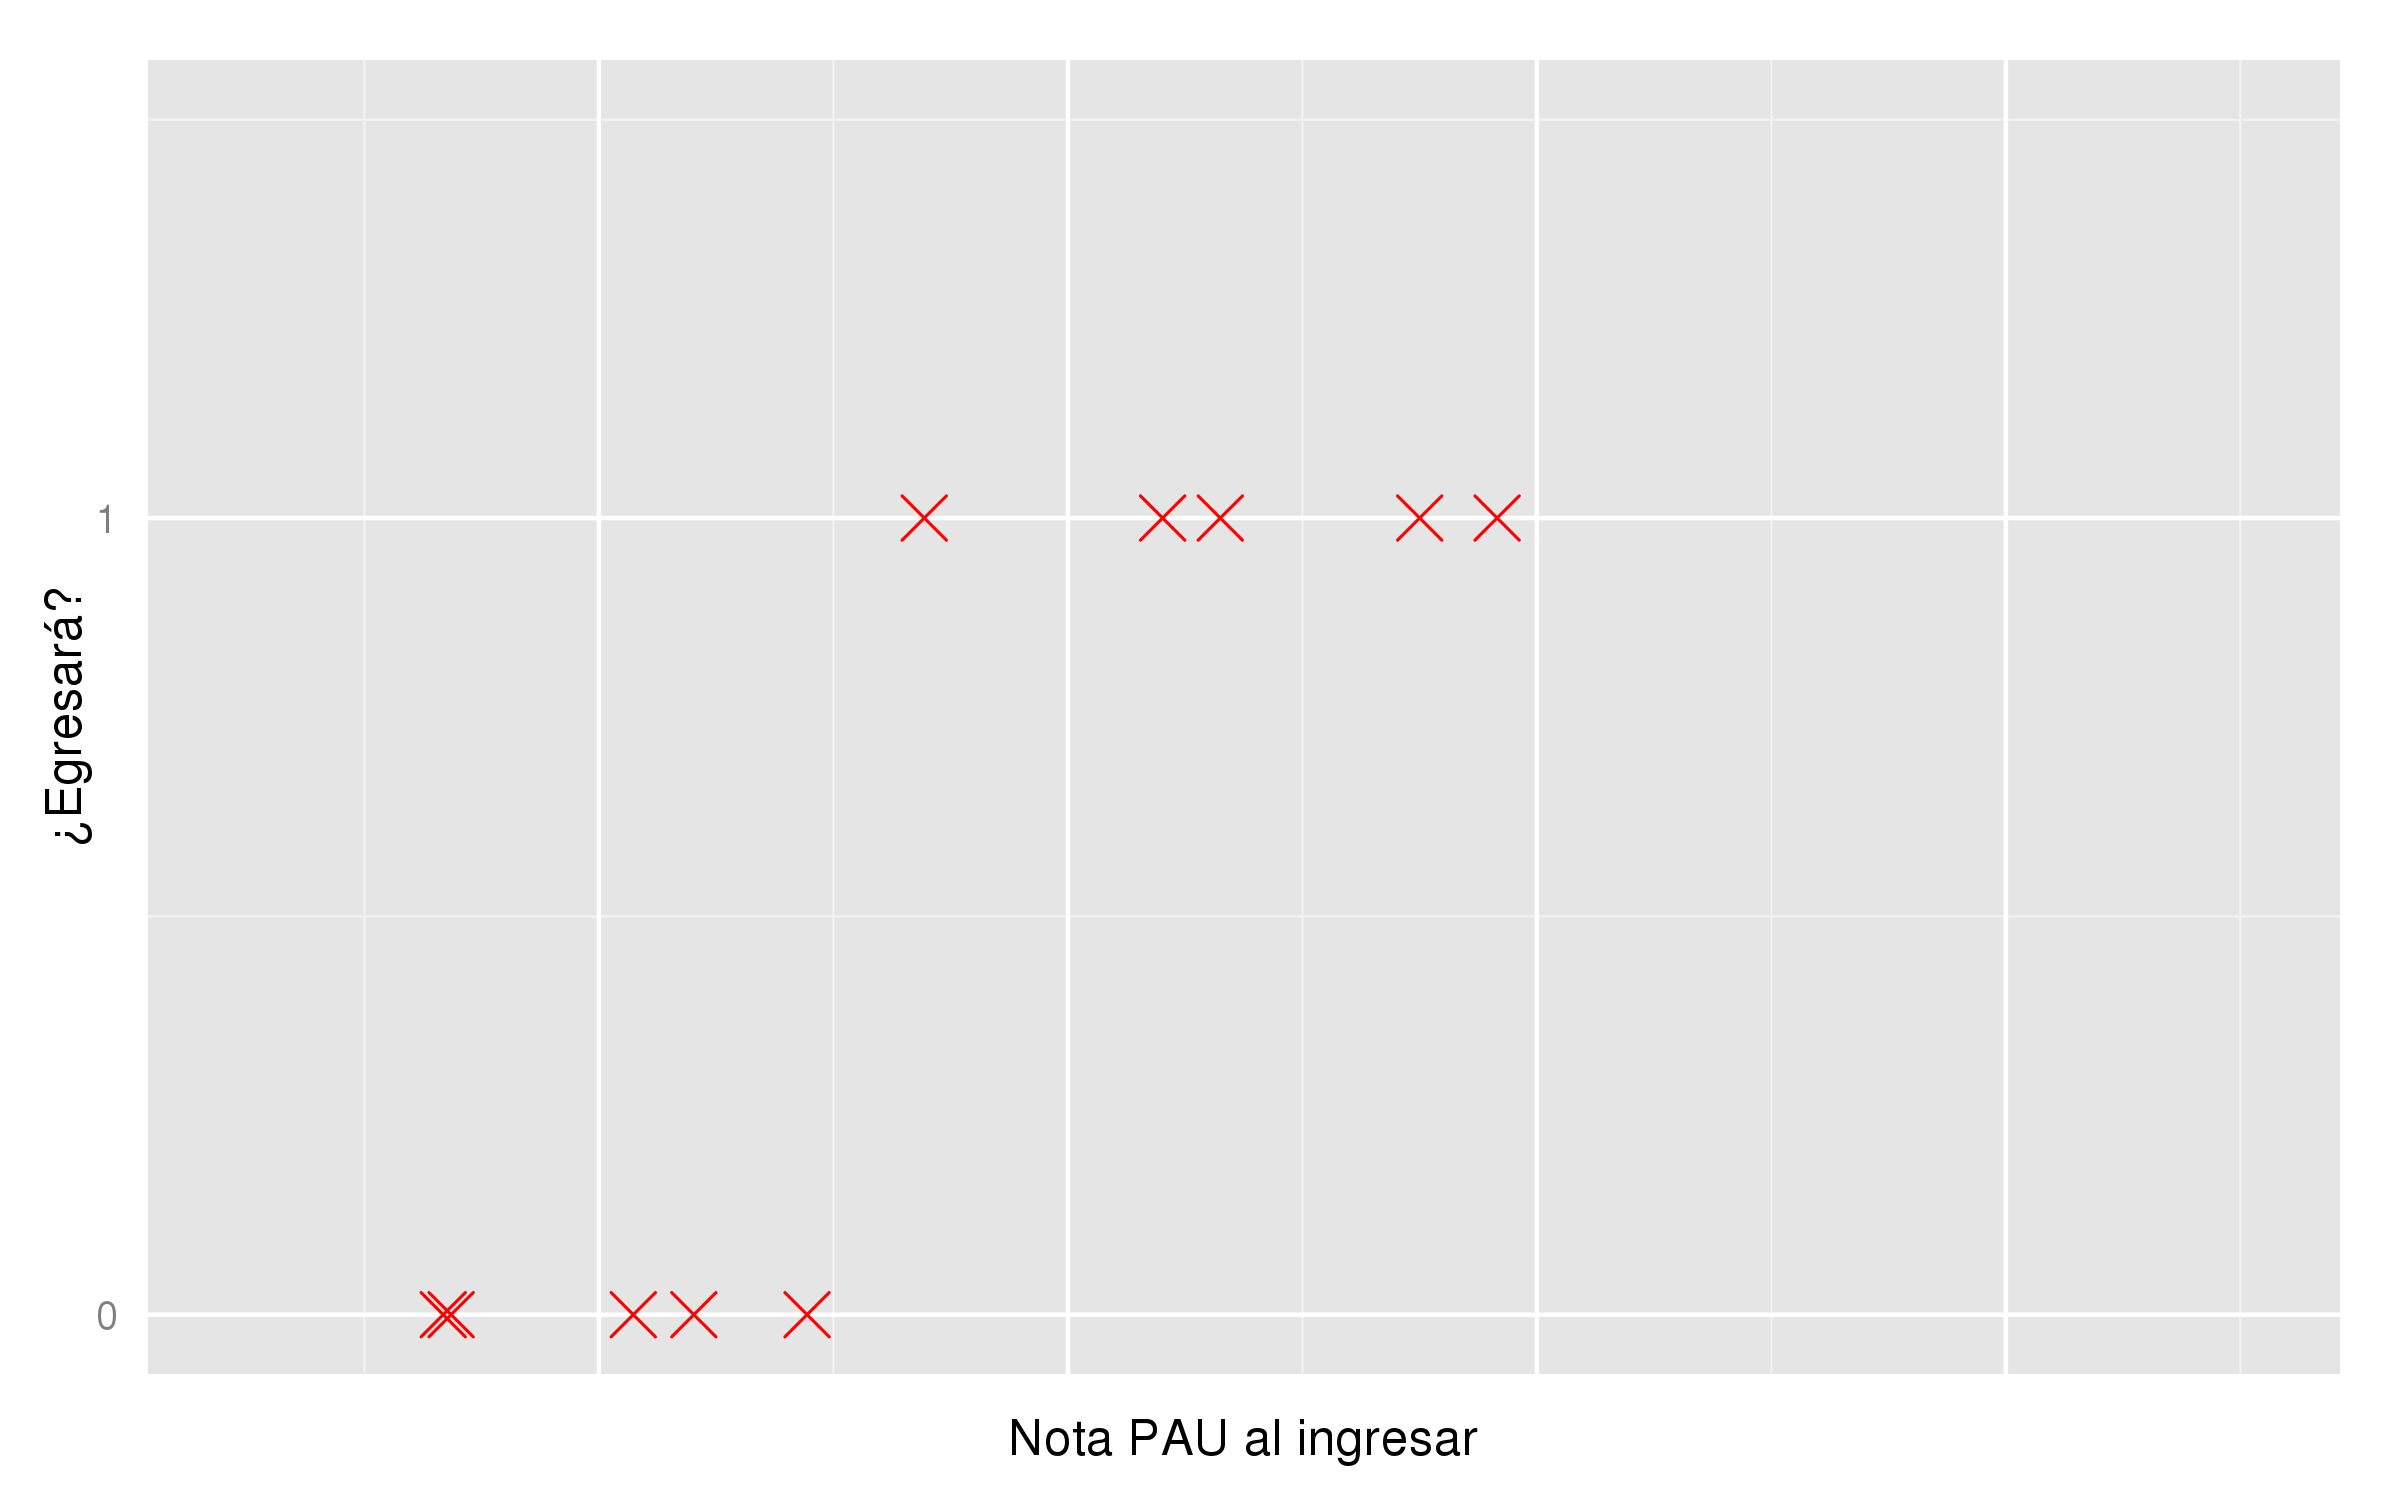
\includegraphics[height=6cm]{egresara1.png}
%% \end{center}
   \end{overlayarea}
   
 \end{frame}
 \section{Ejemplo}
 \begin{frame}\frametitle{Ejemplo: predicción del abandono}
   \begin{overlayarea}{\textwidth}{0.6cm}  
   Codificamos: $y=1\leftrightarrow$ ``Egresará'', $y=0\leftrightarrow$ ``Abandonará''.  
 \end{overlayarea}
 \onslide<2->
\begin{center}
  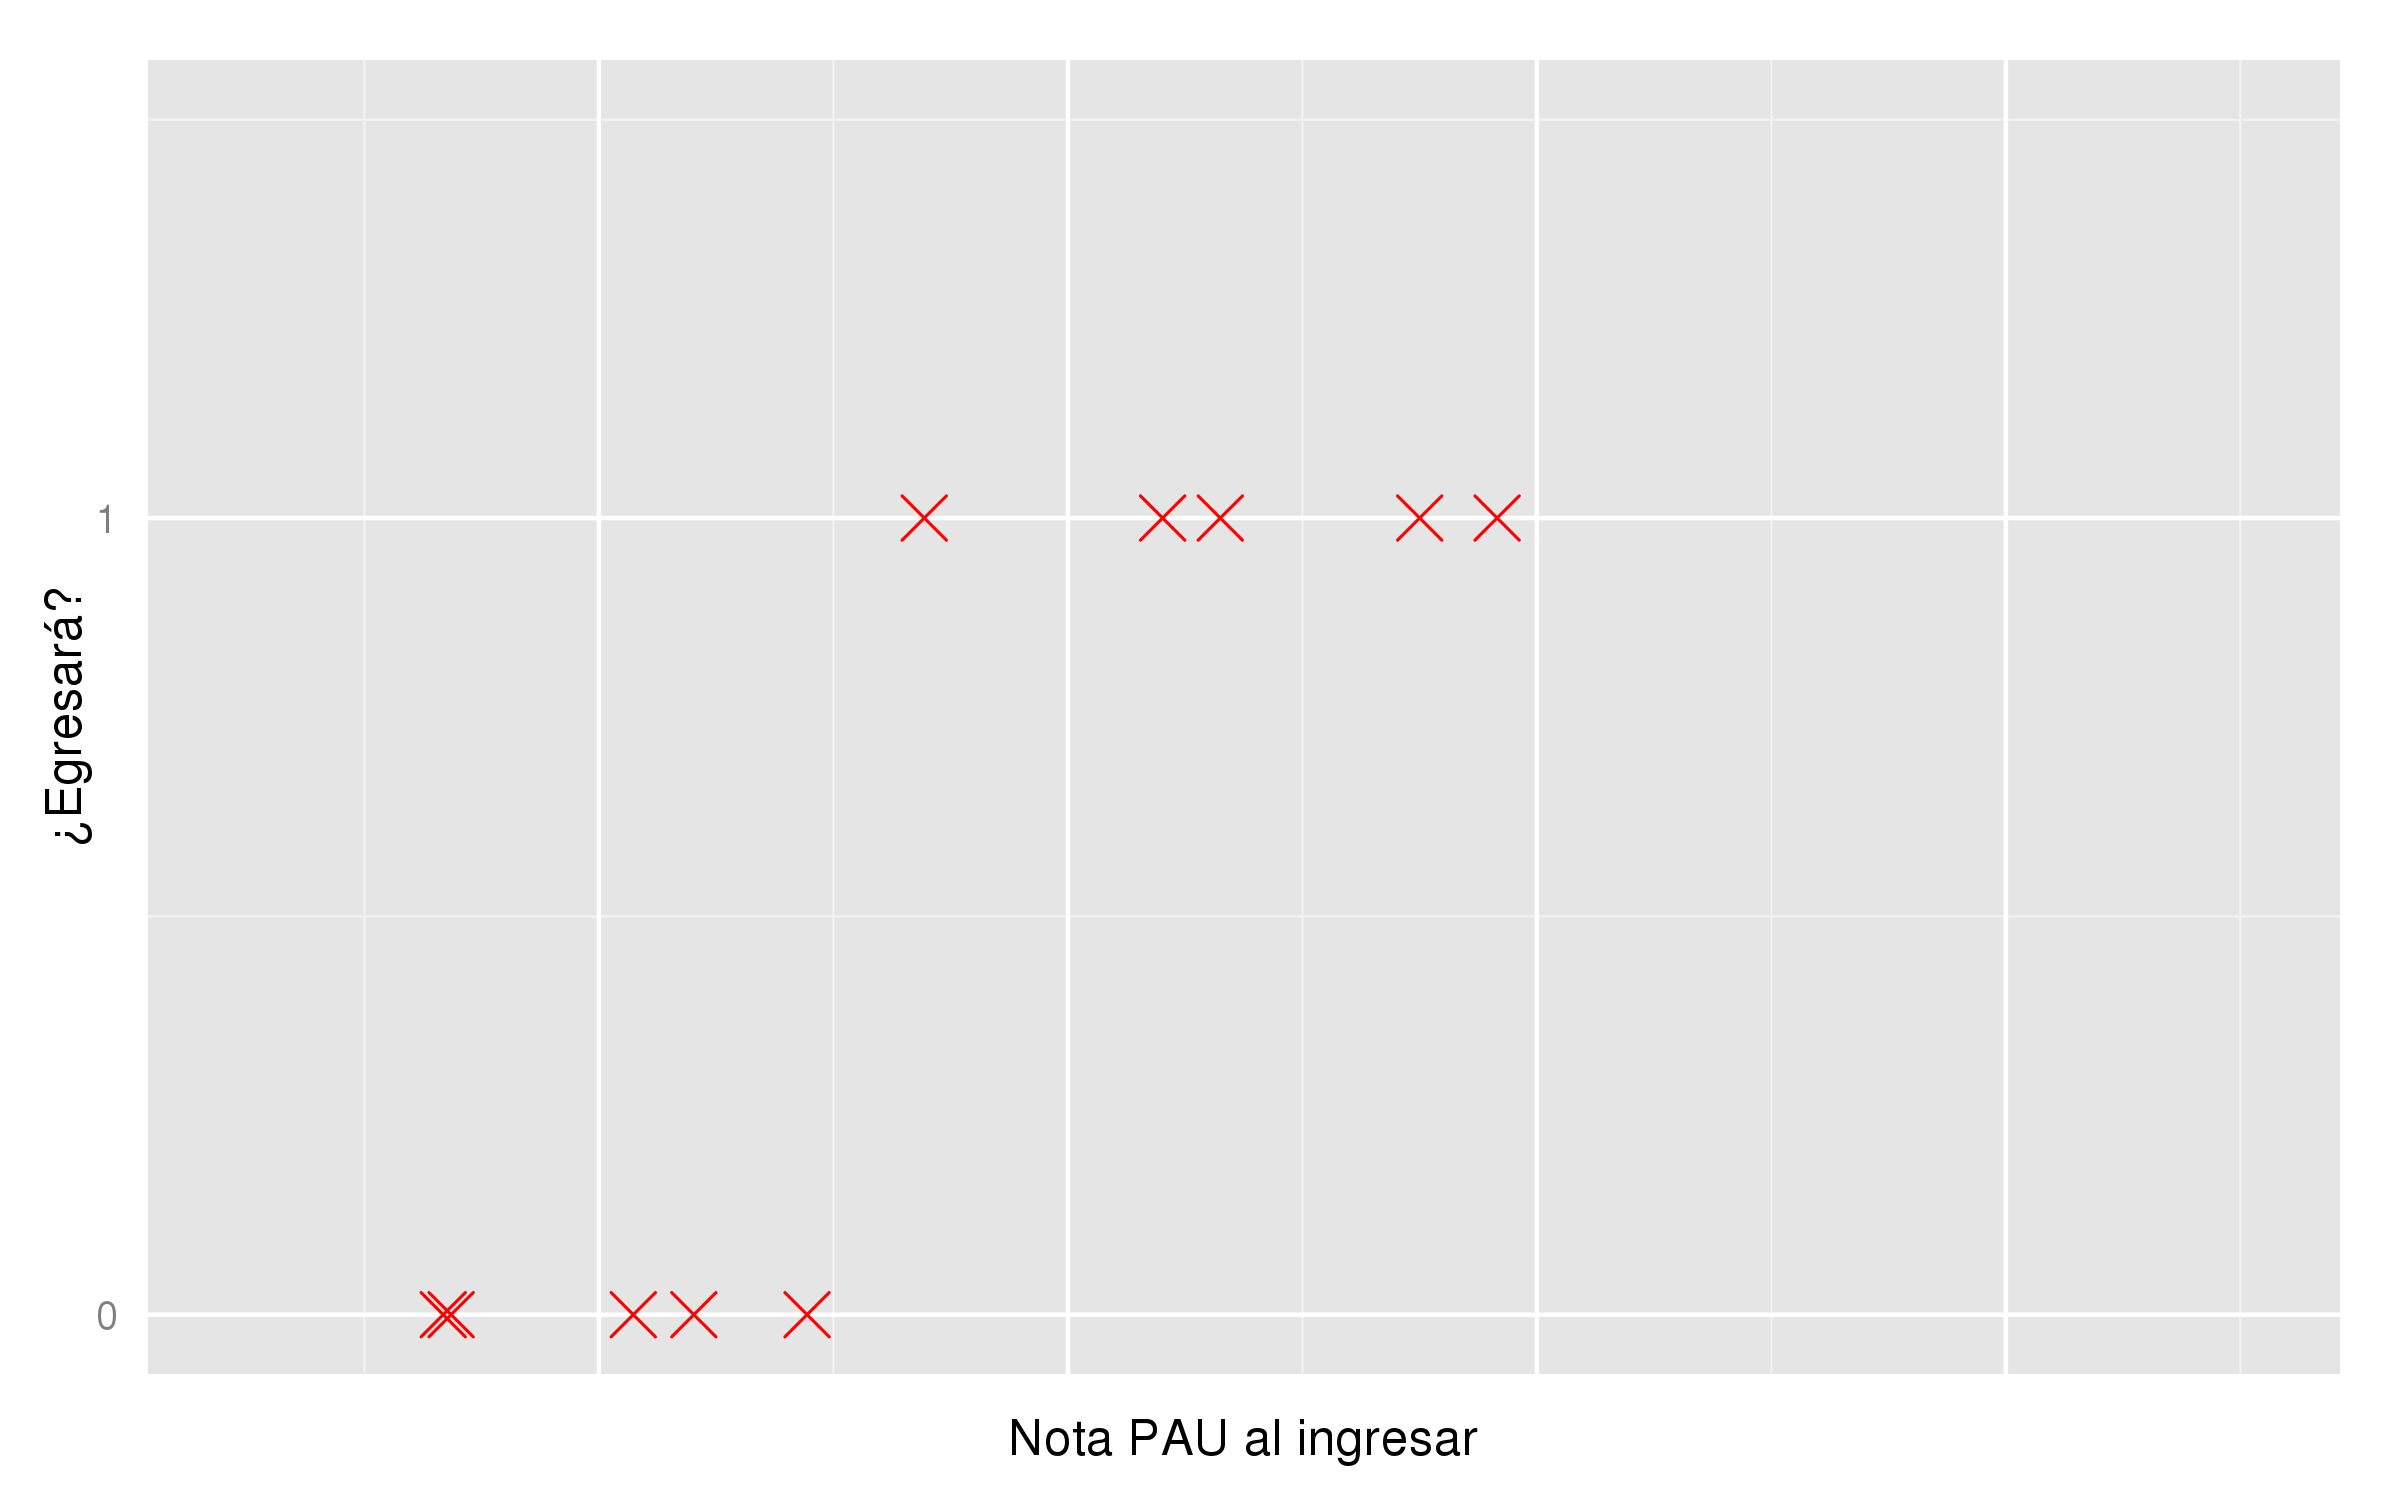
\includegraphics[height=6.6cm]{egresara1.png}
\end{center}
    
 \end{frame}
 
 \begin{frame}\frametitle{Ejemplo: predicción del abandono}
   \begin{overlayarea}{\textwidth}{0.6cm}
  Si usamos regresión lineal, la recta ajustada $y=h_\theta(x)$ es
 \end{overlayarea}
 \begin{center}
  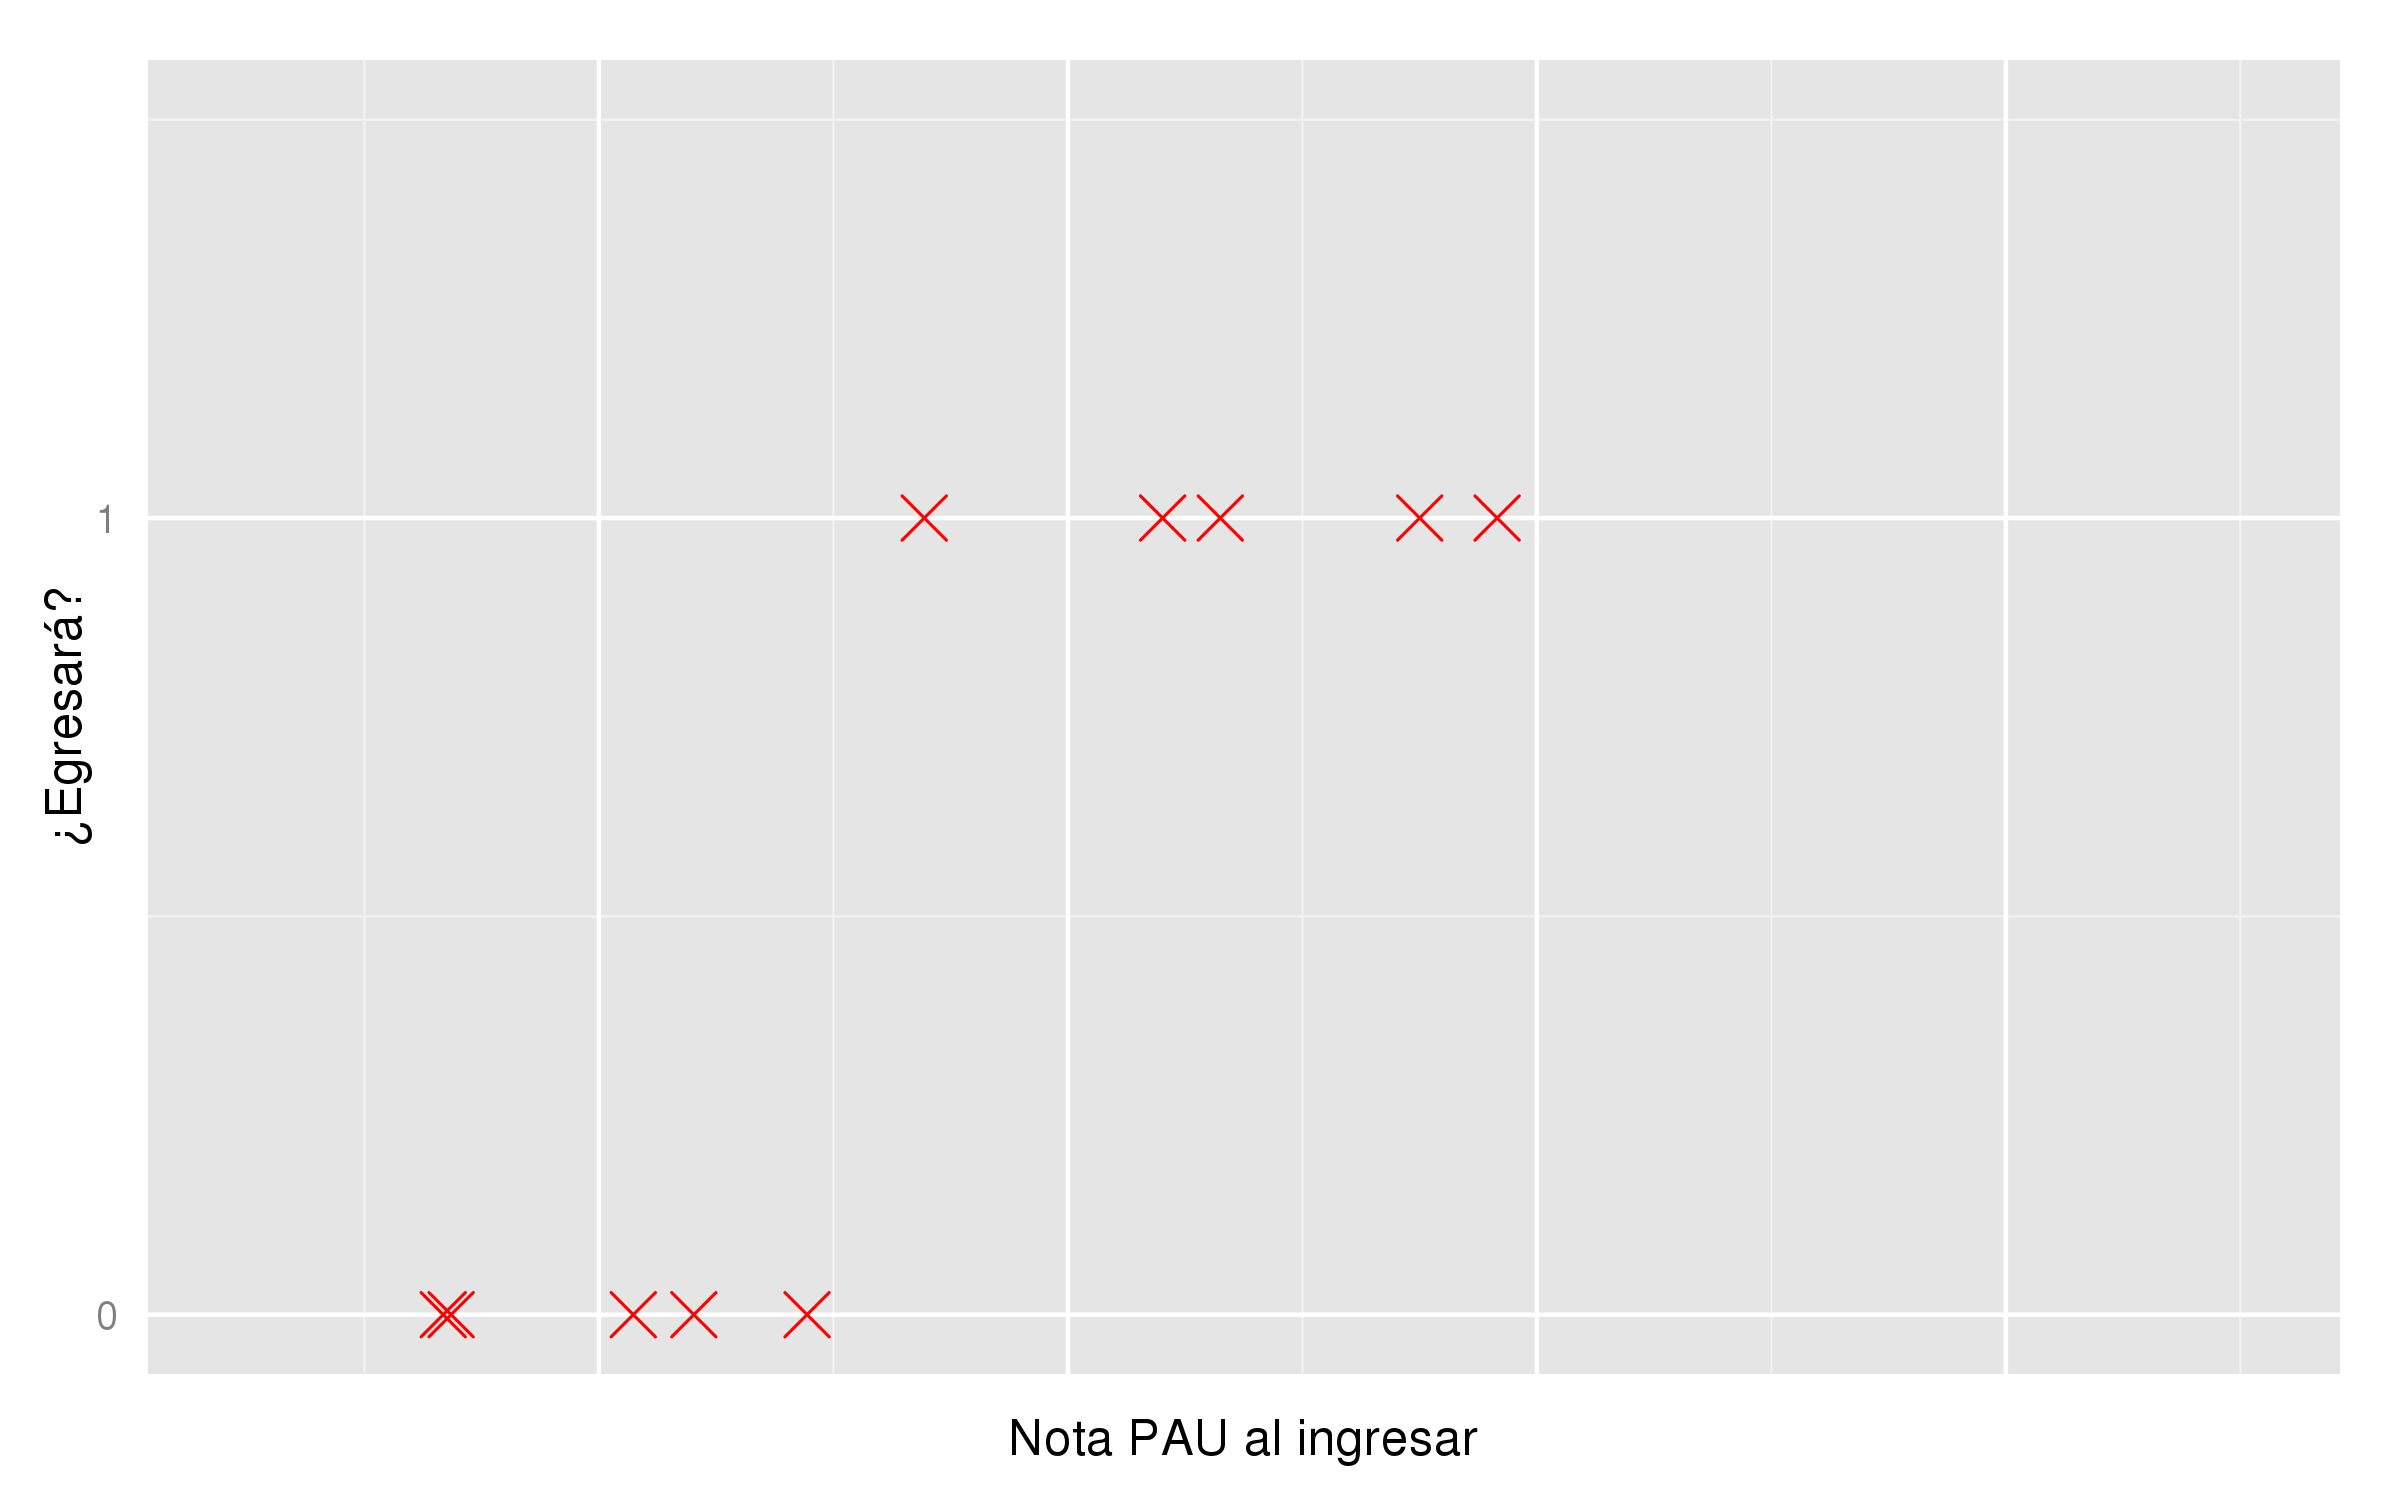
\includegraphics[height=6.6cm]{egresara1.png}
\end{center}
   
 \end{frame}
 \begin{frame}\frametitle{Ejemplo: predicción del abandono}
   \begin{overlayarea}{\textwidth}{0.6cm}  
   Si usamos regresión lineal, la recta ajustada $y=h_\theta(x)$ es
 \end{overlayarea}
 \begin{center}
  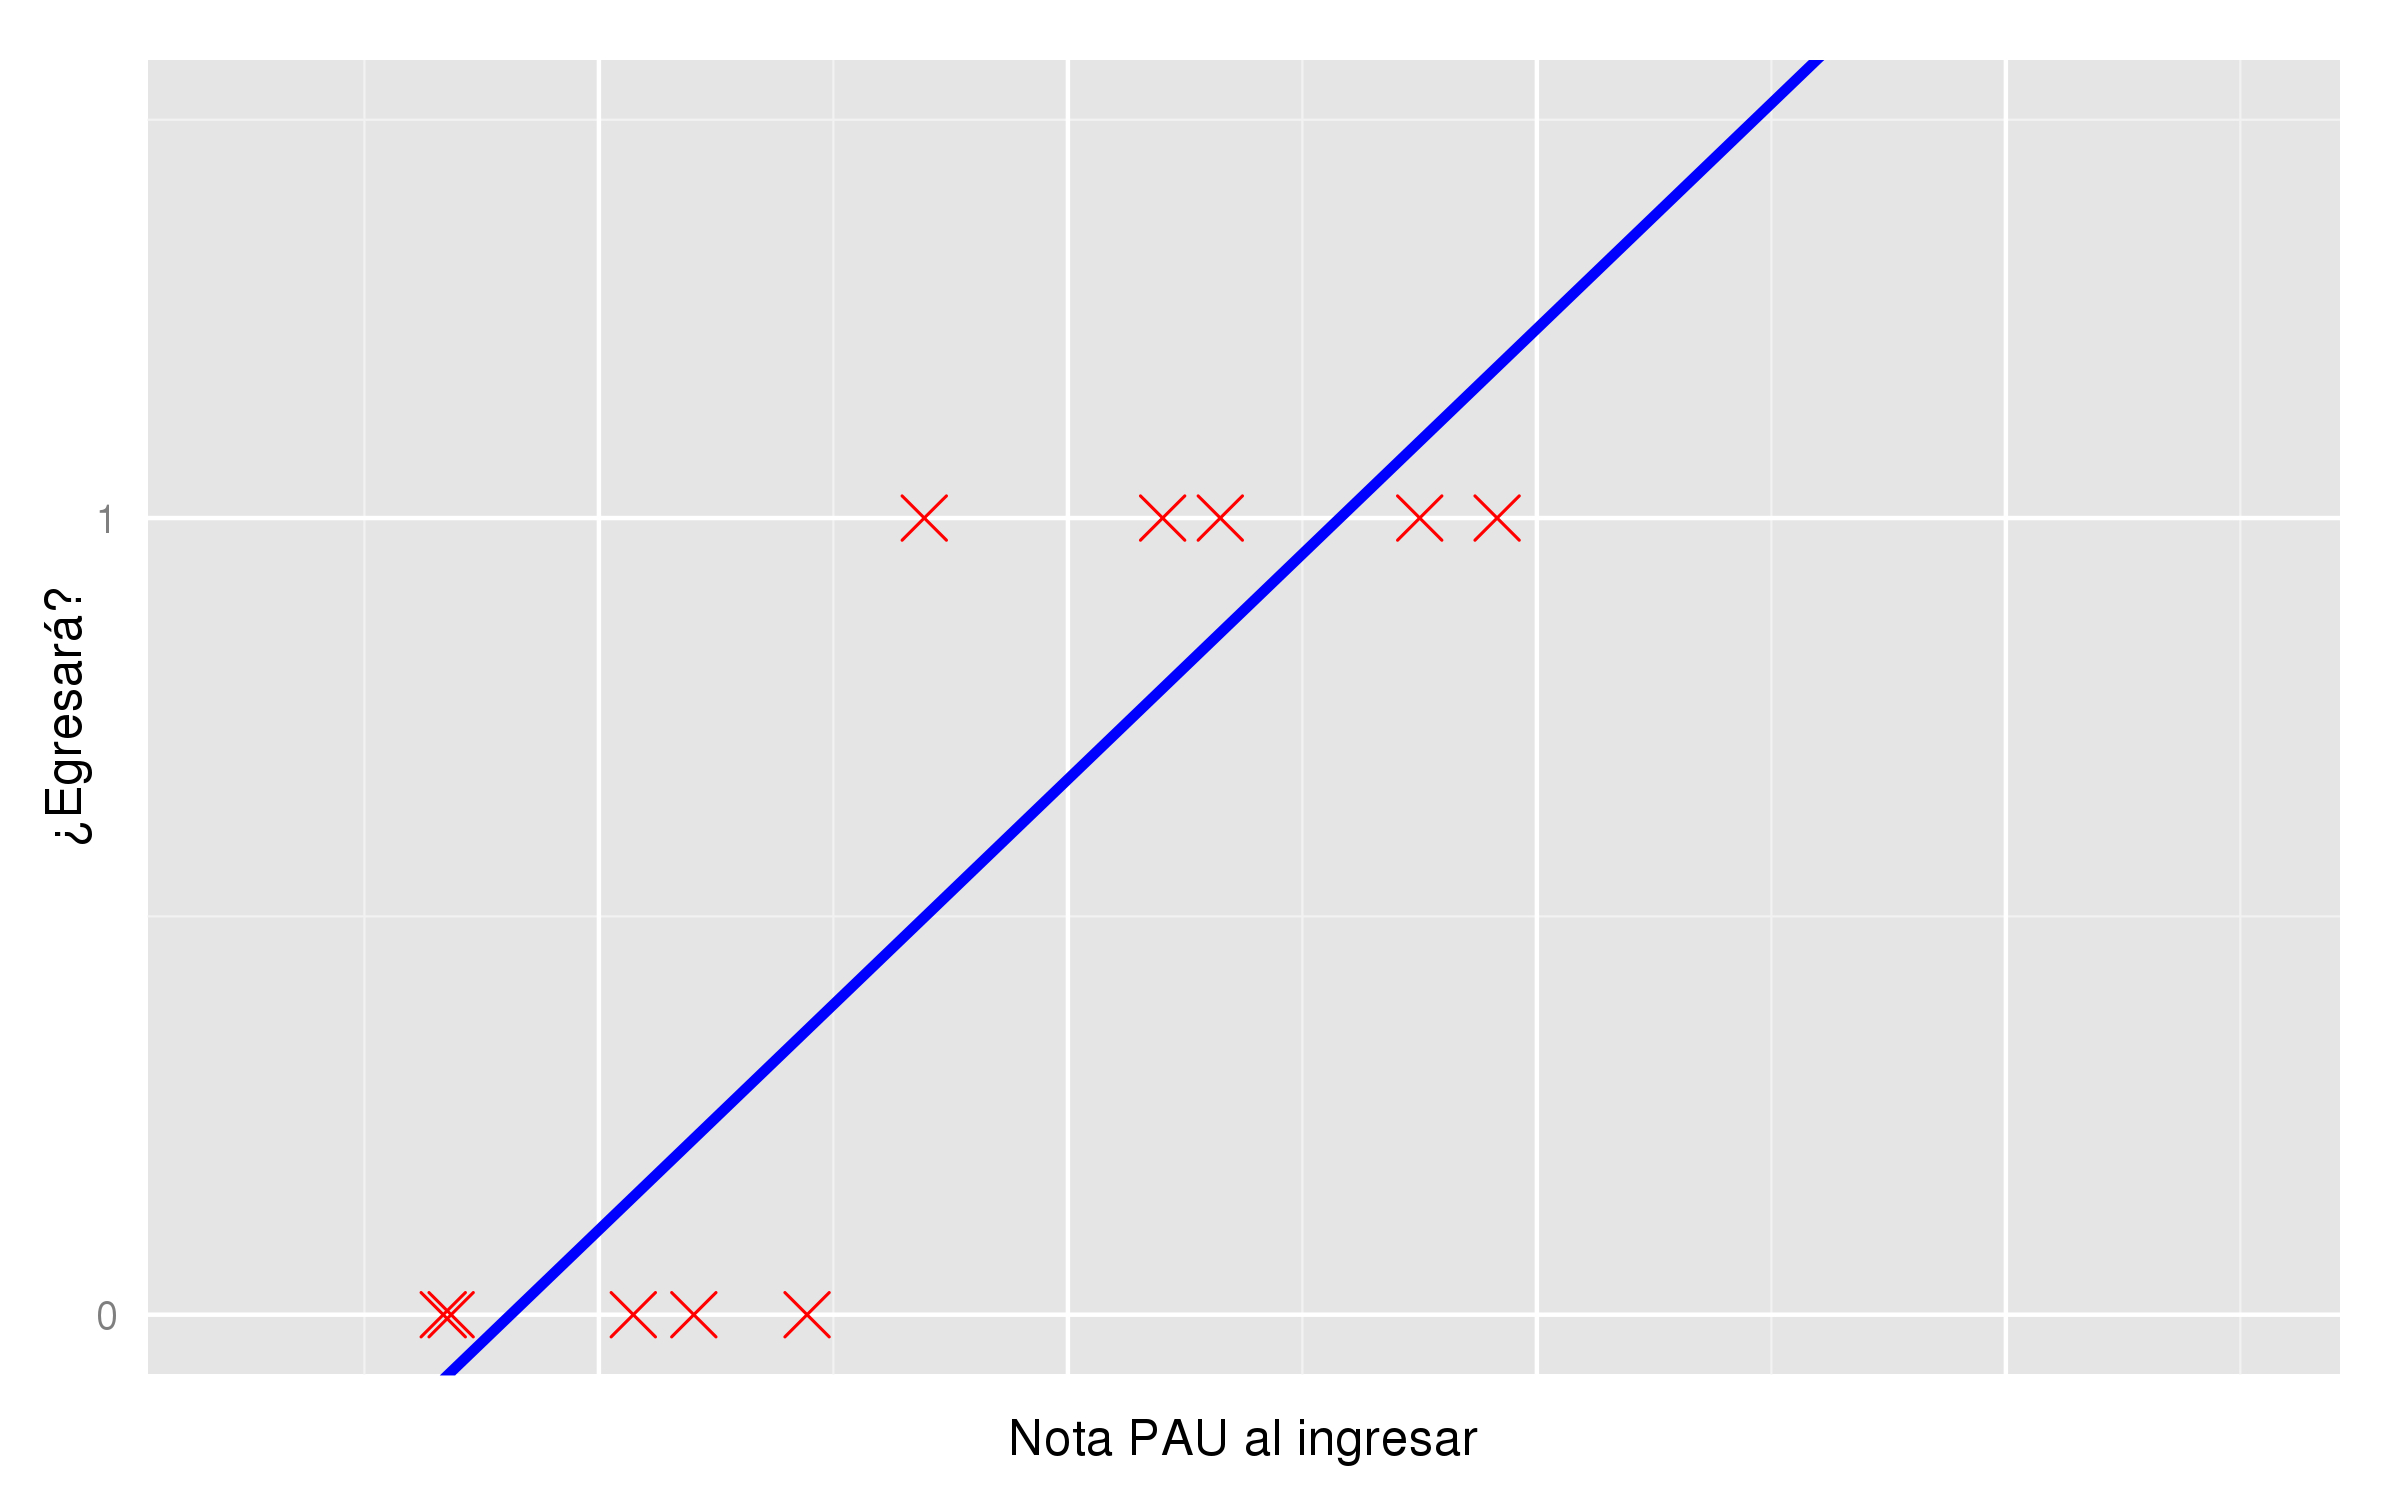
\includegraphics[height=6.6cm]{egresara2.png}
\end{center}
  \end{frame}
  
 \begin{frame}\frametitle{Ejemplo: predicción del abandono}
   \begin{overlayarea}{\textwidth}{0.6cm}
   Si usamos regresión lineal, la recta ajustada $y=h_\theta(x)$ es 
 \end{overlayarea}
 \begin{center}
  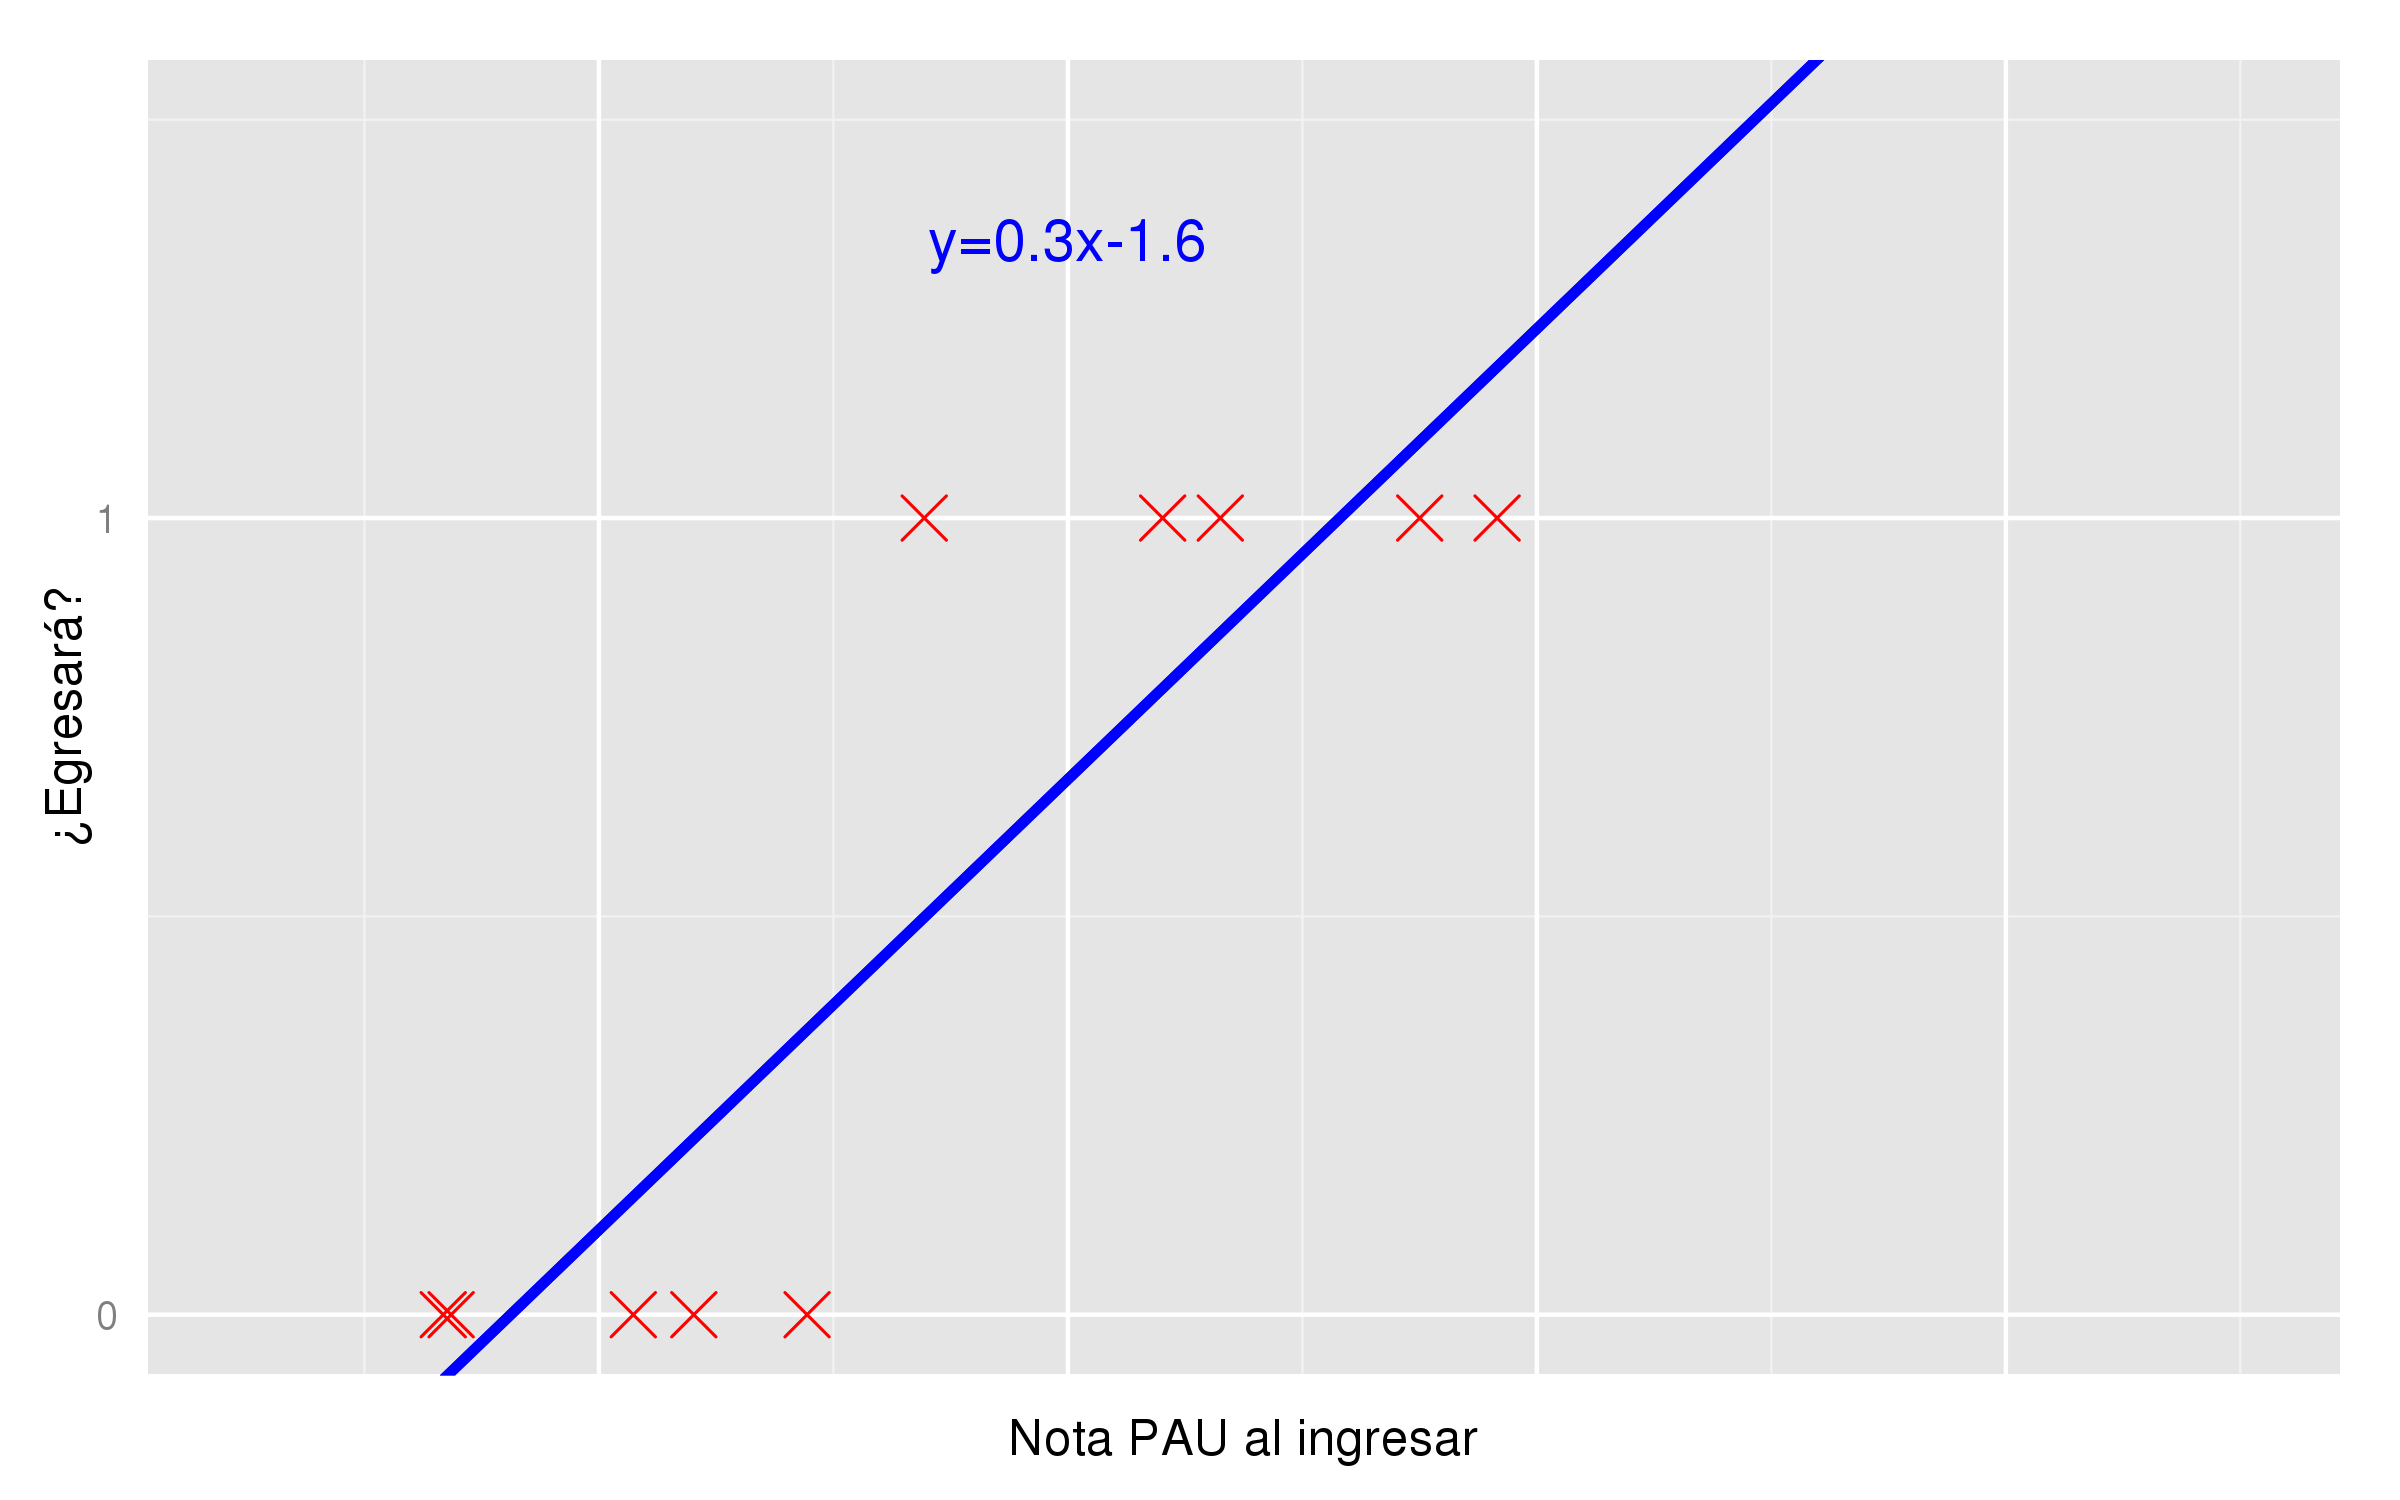
\includegraphics[height=6.6cm]{egresara3.png}
\end{center}
  \end{frame}
  
 \begin{frame}\frametitle{Ejemplo: predicción de abandono}
   \begin{overlayarea}{\textwidth}{\textheight}  
     ¿ Podemos usar esta recta ajustada $y=0.3x-1.6$ para hacer predicción ante un nuevo alumno que ingresa?  \\
     \onslide<+-> ¡Sí! Podemos aprovecharla para definir una regla de decisión:
     \begin{enumerate}
     \item<+-> Sustituimos la nota PAU de ingreso del nuevo alumno en la ecuación ajustada. Obtenemos $\Rightarrow \hat y$.
     \item<+-> Si $\hat y> 0.5$, predecimos que egresará.
     \item<+-> Si $\hat y< 0.5$, predecimos que abandonará.
     \end{enumerate}
   \end{overlayarea}
 \end{frame}
 \begin{frame}\frametitle{Ejemplo: predicción del abandono}
   \begin{overlayarea}{\textwidth}{0.6cm}
   Gráficamente, nuestro criterio de decisión sobre $\hat{y}$: 
 \end{overlayarea}
 \begin{center}
  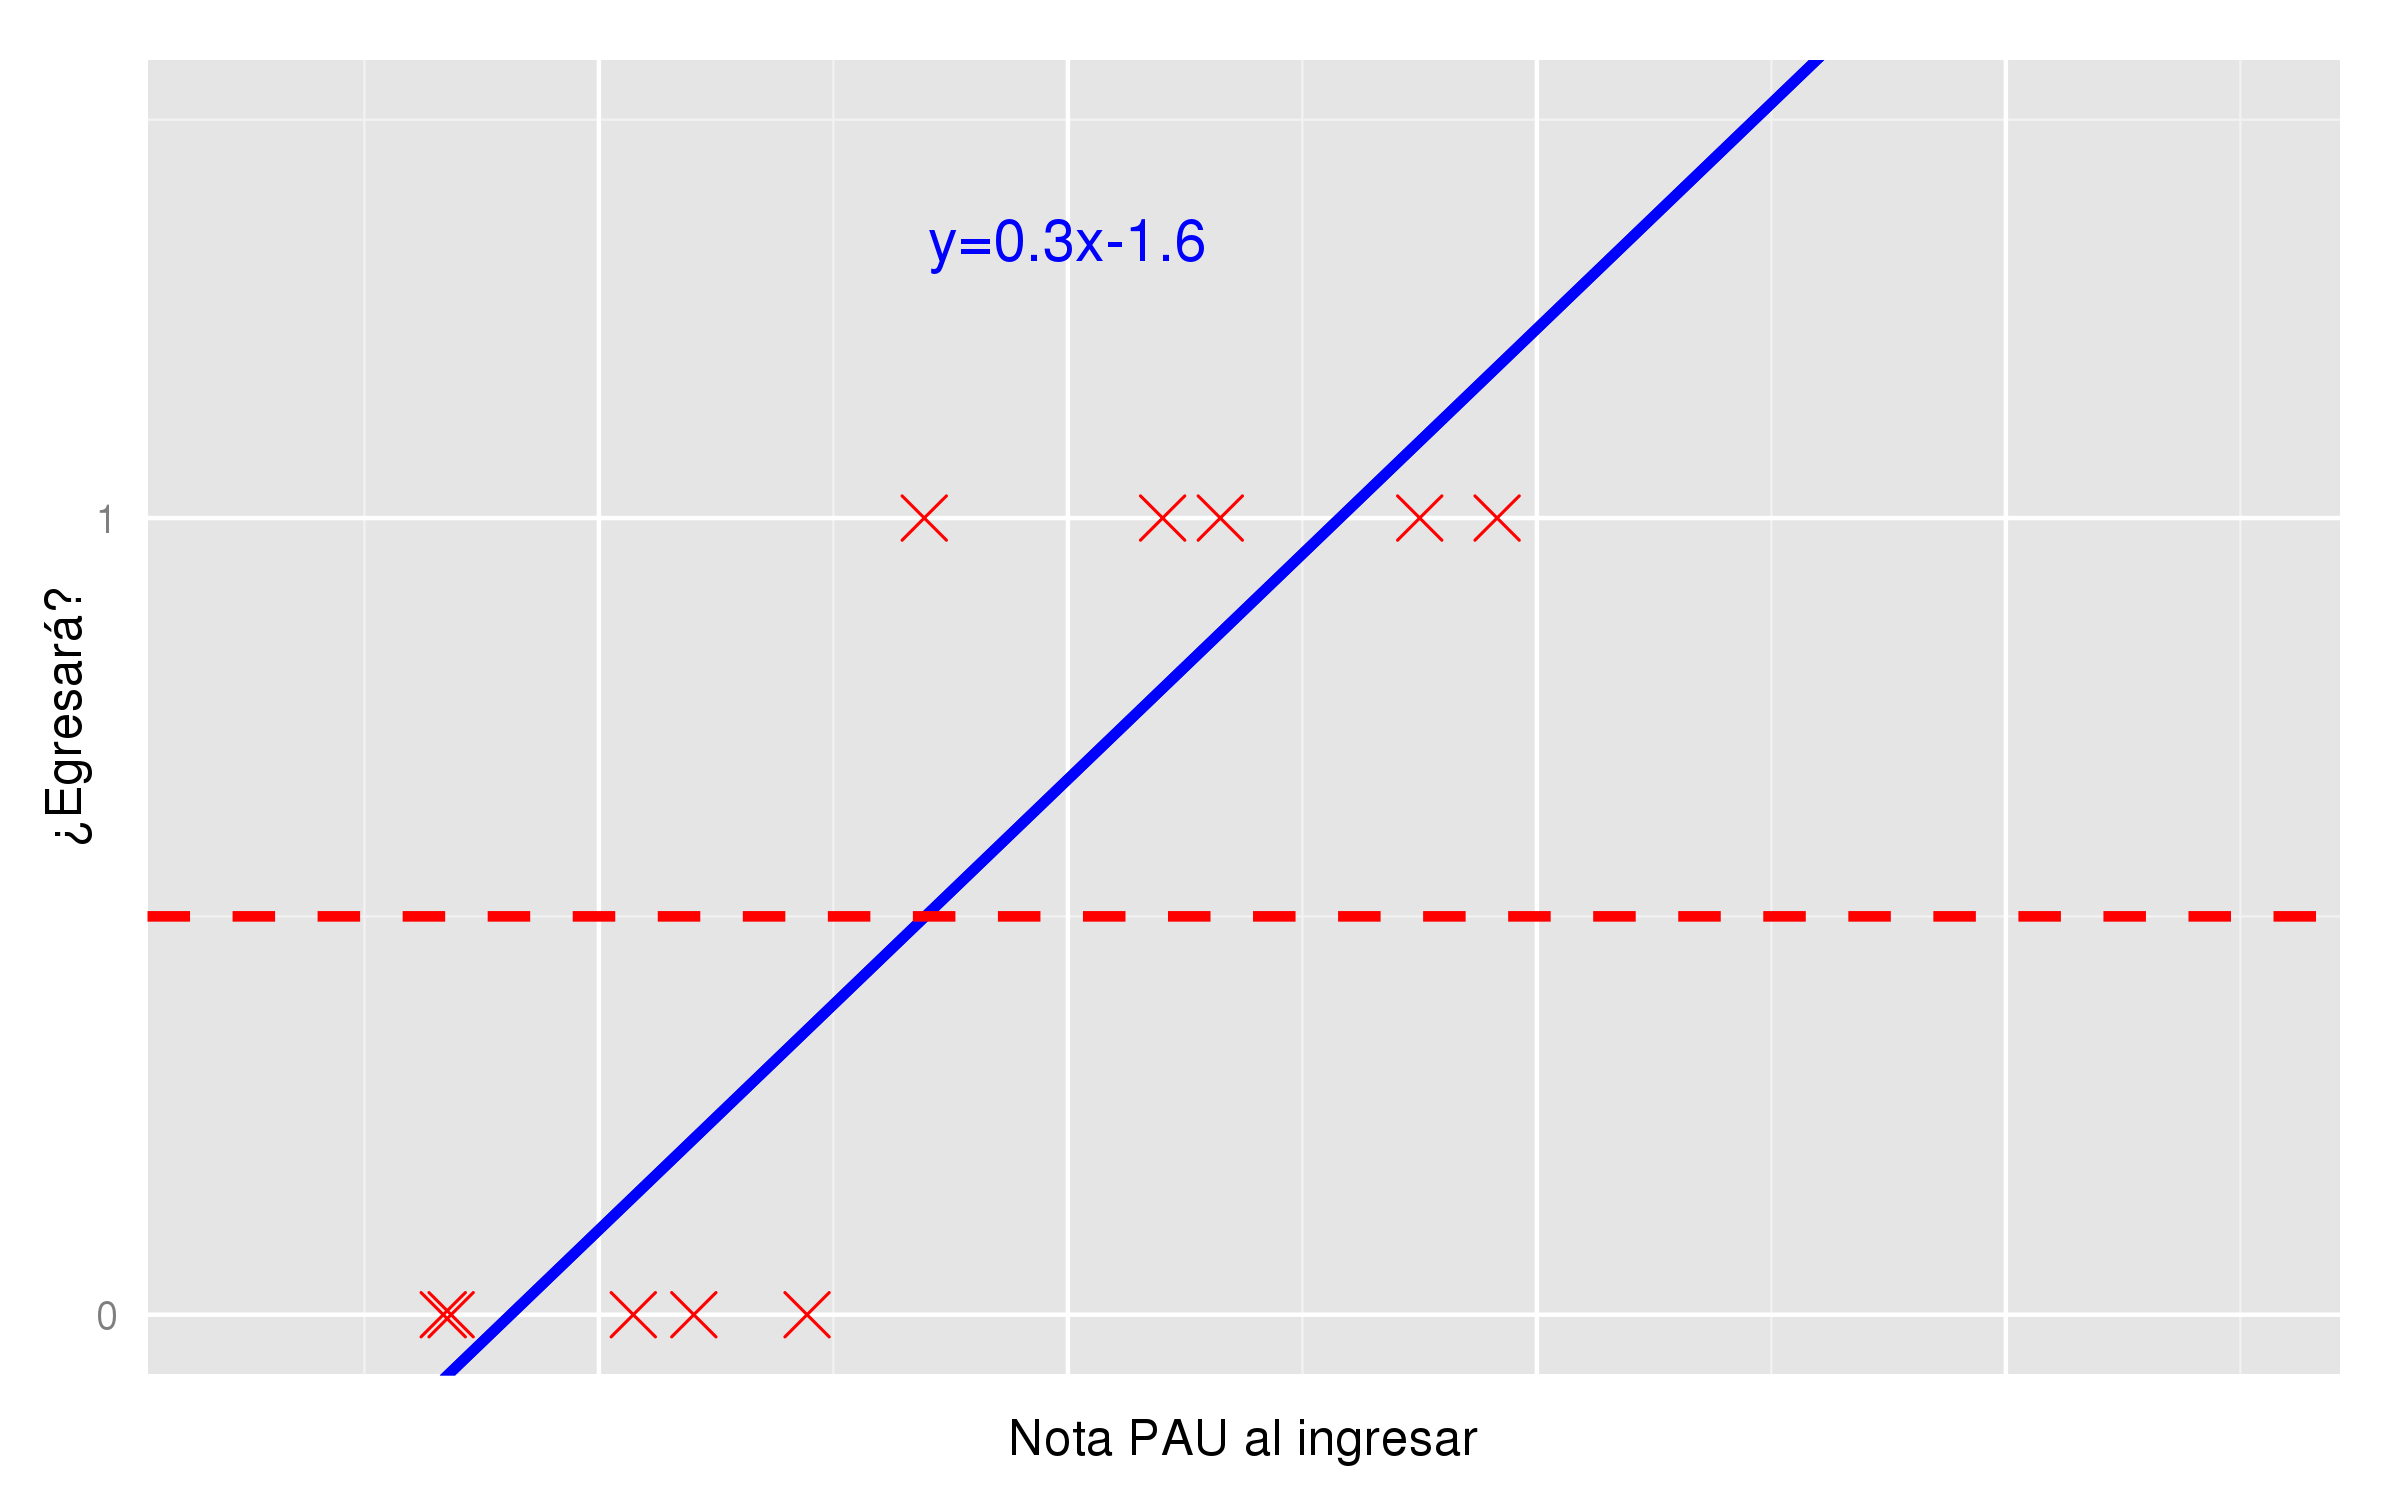
\includegraphics[height=6.6cm]{egresara4.png}
\end{center}
  \end{frame}
  
 \begin{frame}\frametitle{Ejemplo: predicción del abandono}
   \begin{overlayarea}{\textwidth}{0.6cm}  
   Gráficamente, nuestro criterio de decisión sobre $\hat{y}$: 
 \end{overlayarea}
 \begin{center}
  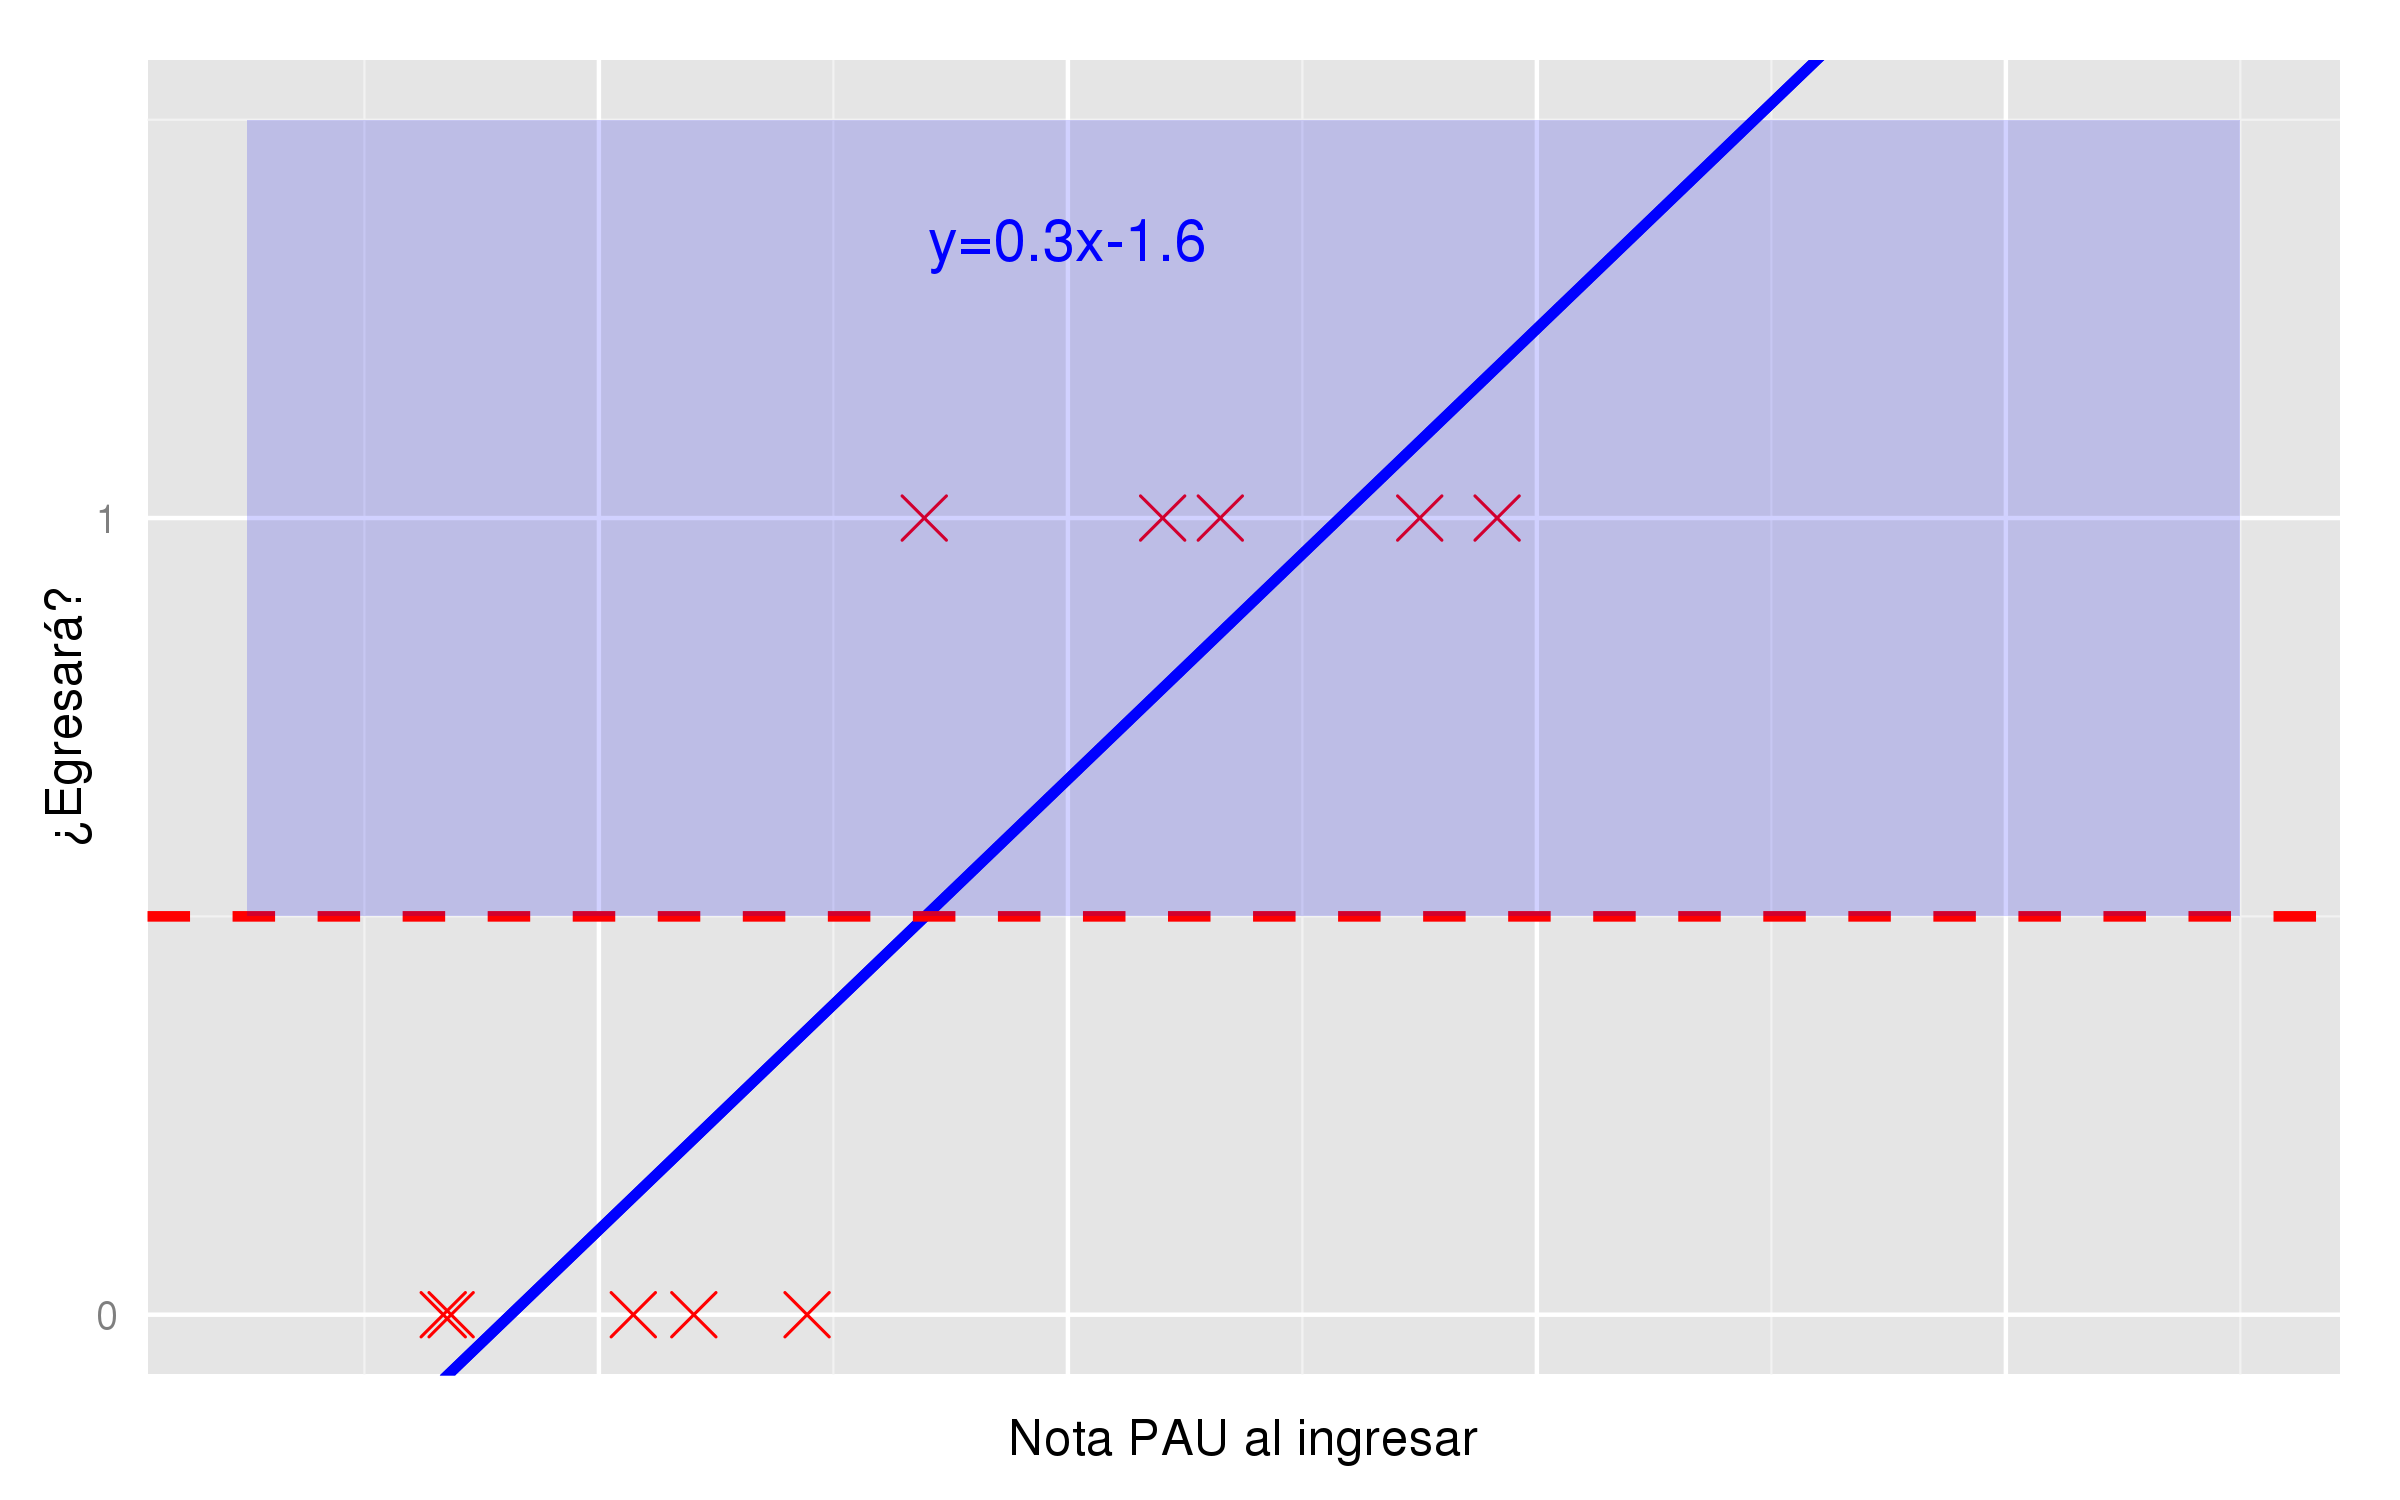
\includegraphics[height=6.6cm]{egresara5.png}
\end{center}
  \end{frame}
  
 \begin{frame}\frametitle{Ejemplo: predicción del abandono}
   \begin{overlayarea}{\textwidth}{0.6cm}  
   Gráficamente, nuestro criterio de decisión sobre $\hat{y}$:
 \end{overlayarea}
 \begin{center}
  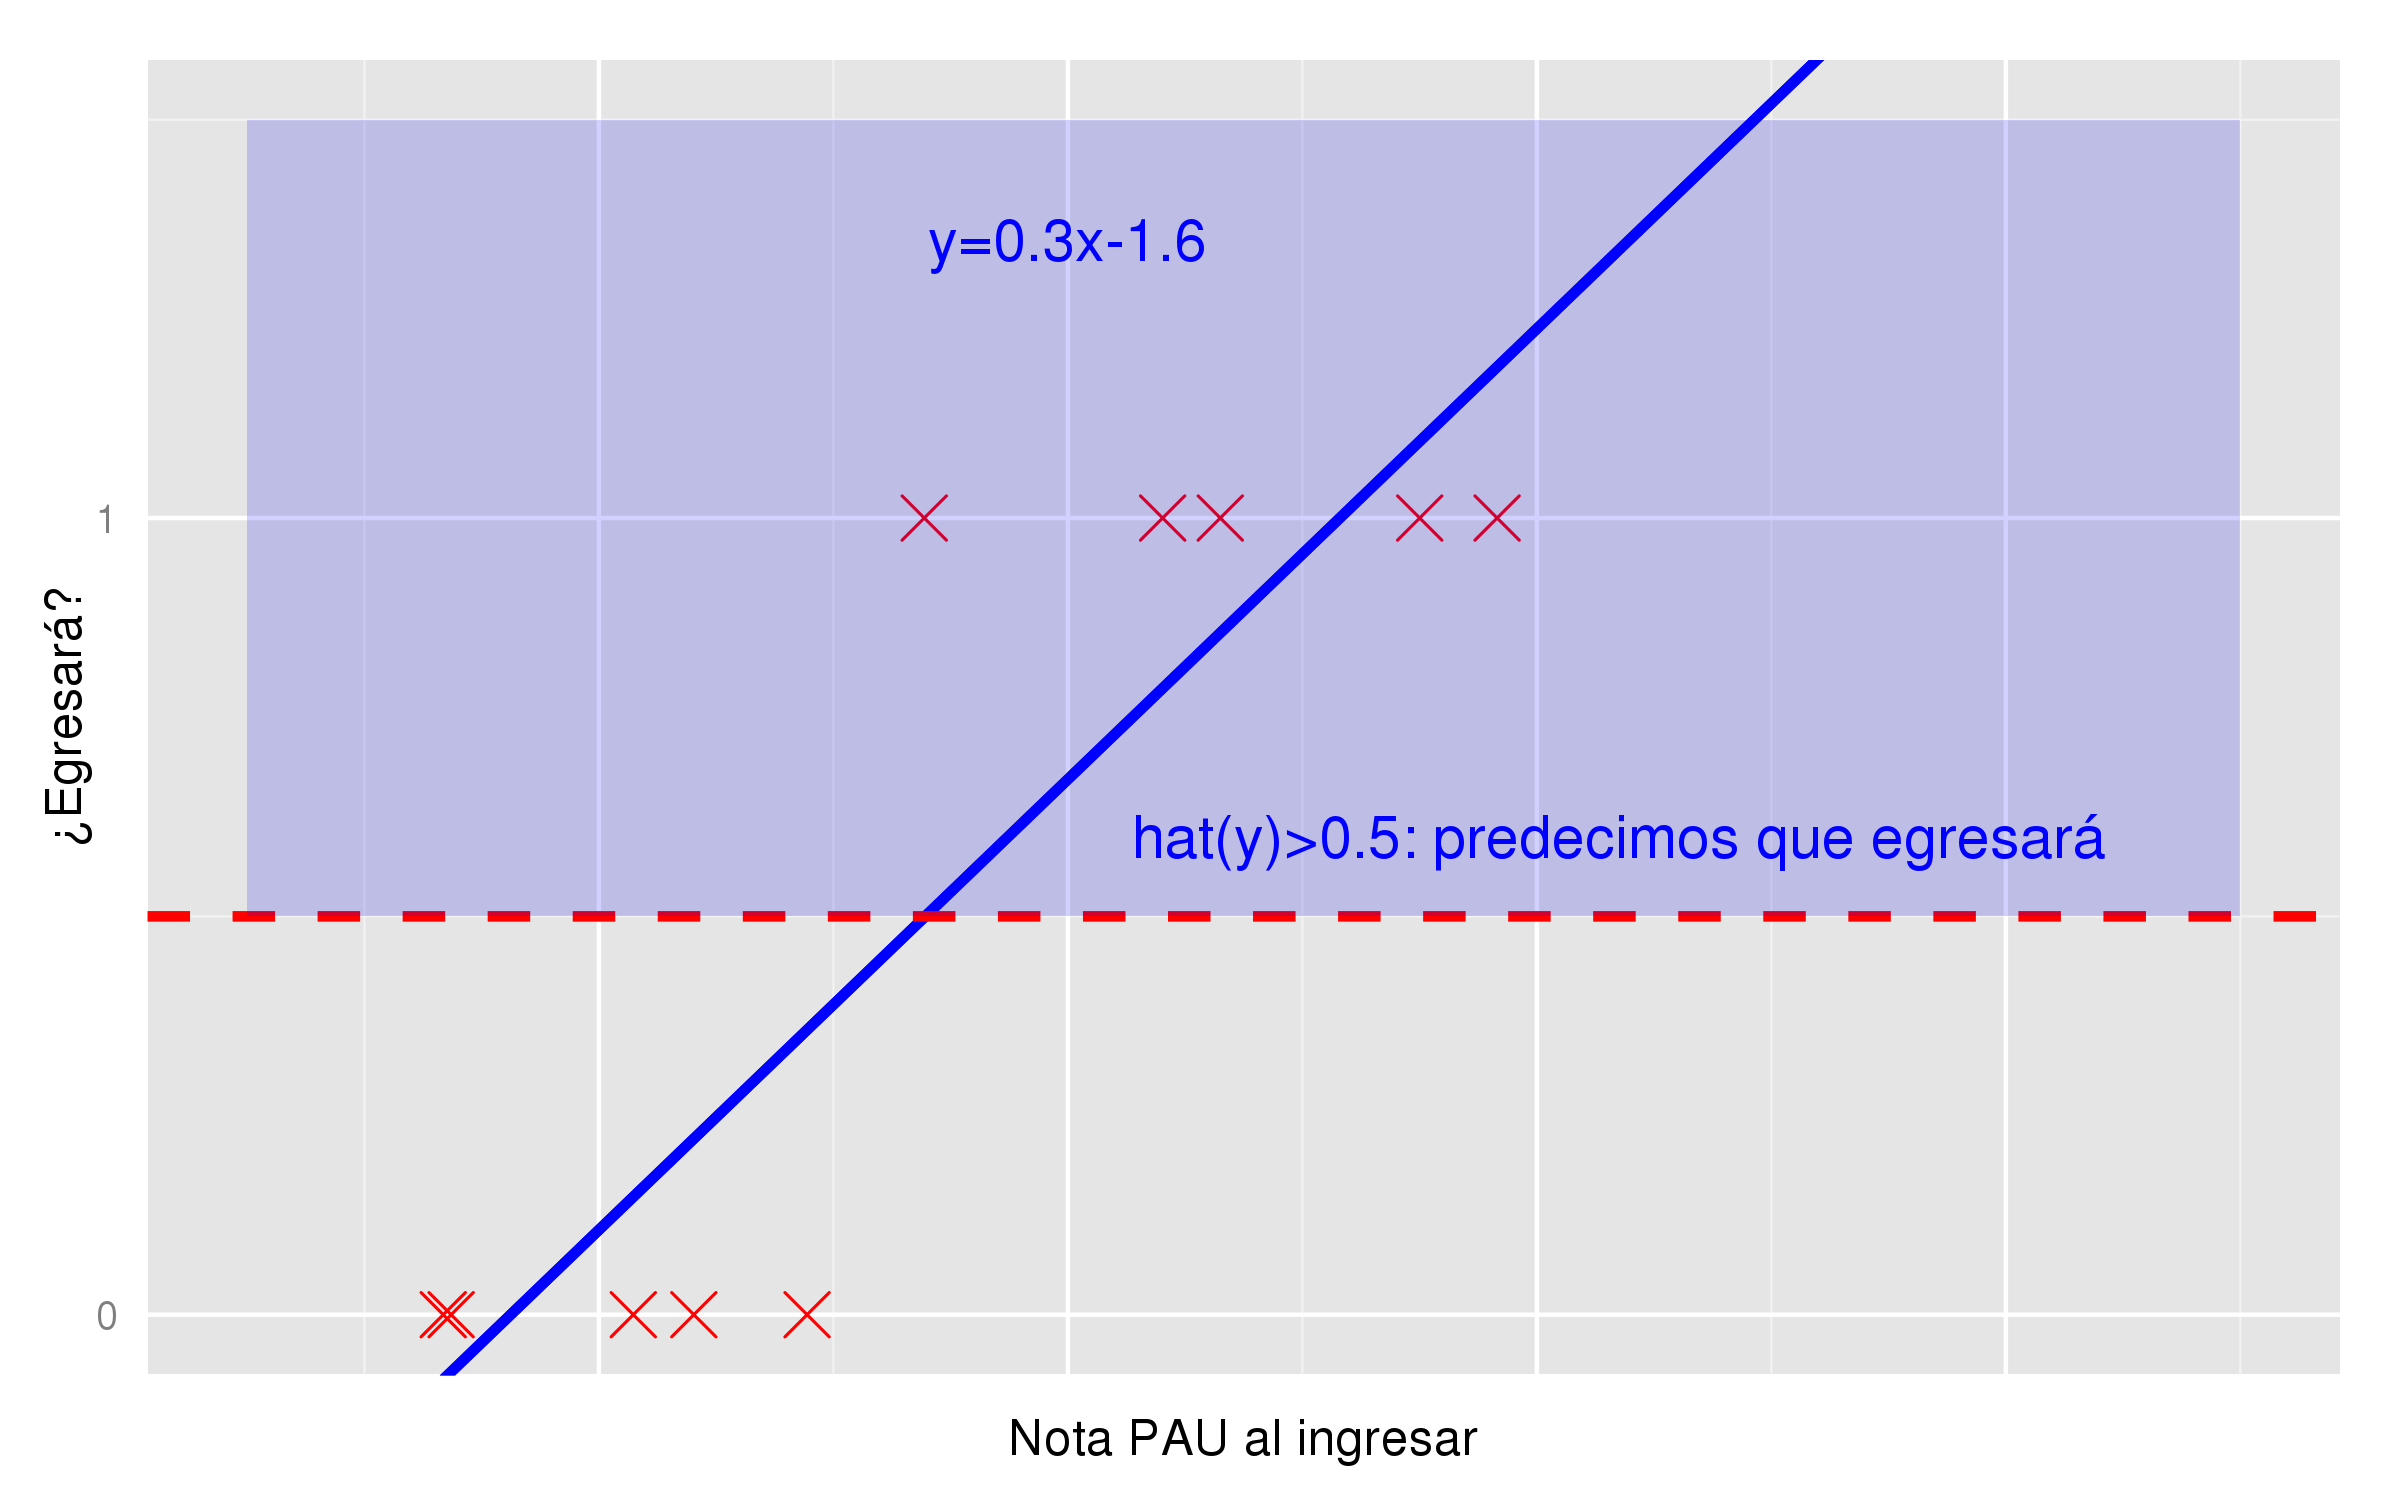
\includegraphics[height=6.6cm]{egresara6.png}
\end{center}
  \end{frame}
  
 \begin{frame}\frametitle{Ejemplo: predicción del abandono}
   \begin{overlayarea}{\textwidth}{0.6cm}  
   Lo traducimos en términos de $x$, : 
 \end{overlayarea}
 \begin{center}
  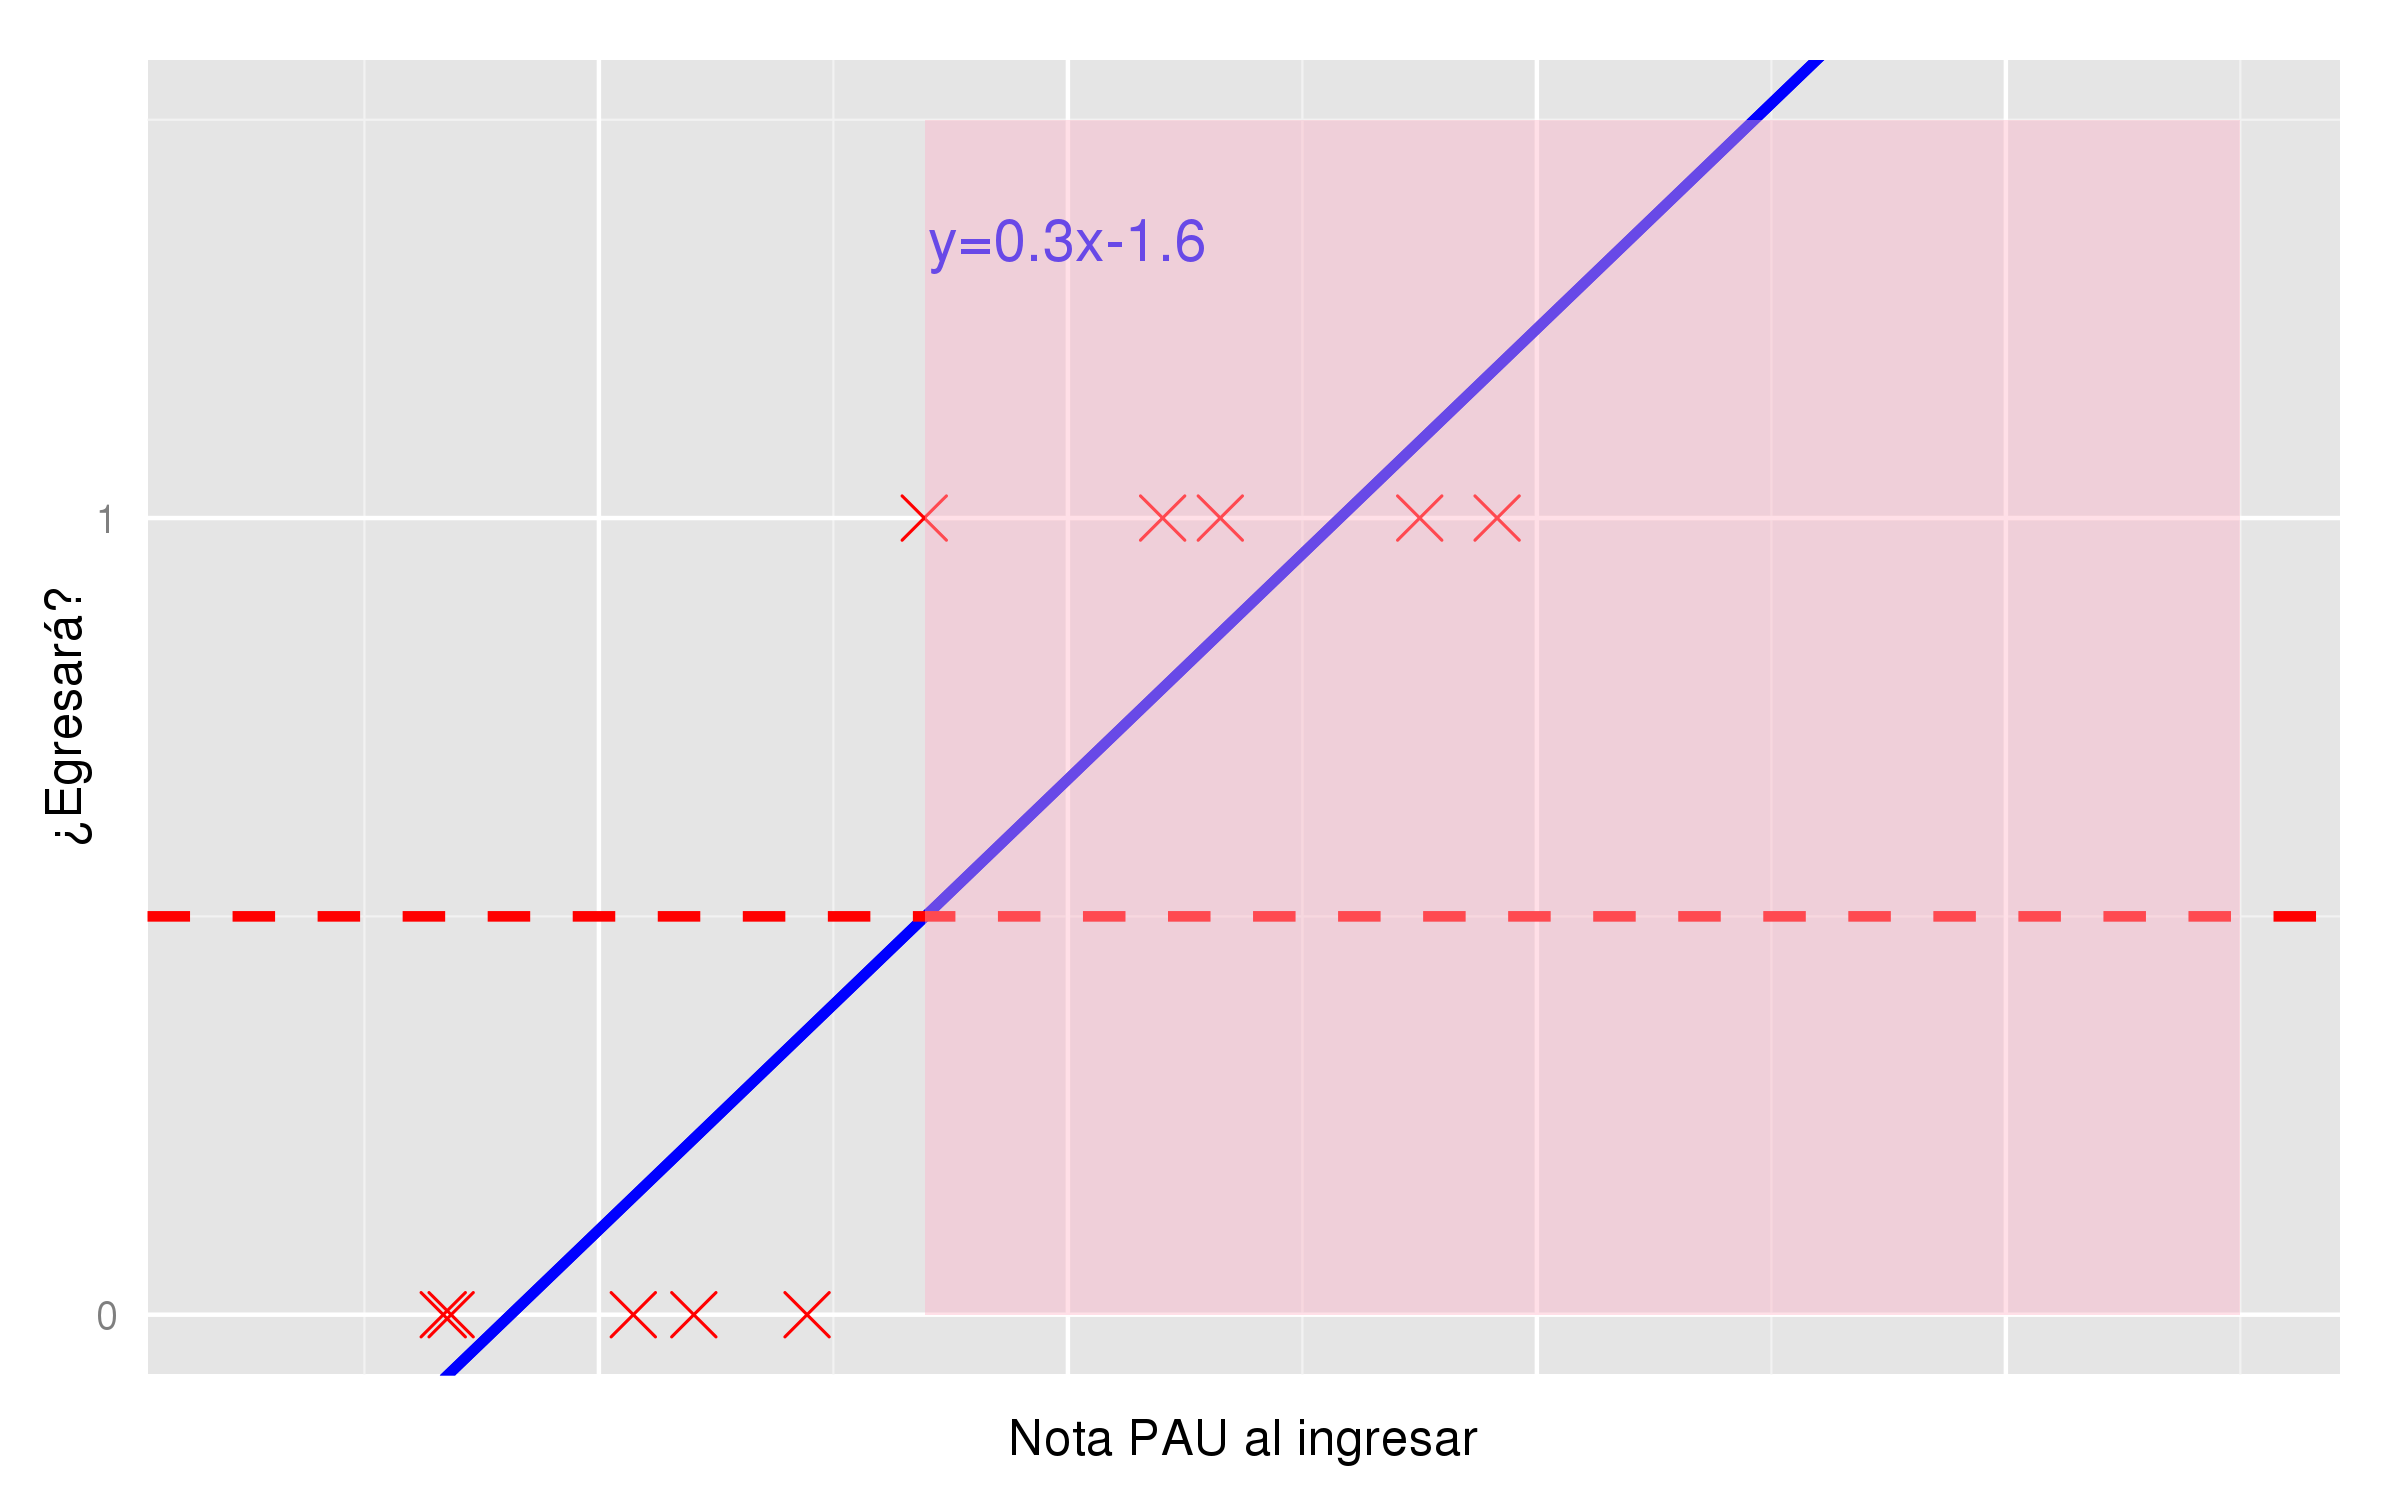
\includegraphics[height=6.6cm]{egresara7.png}
\end{center}
 
 \end{frame}
 \begin{frame}\frametitle{Ejemplo: predicción del abandono}
   \begin{overlayarea}{\textwidth}{0.6cm}    
   Decir $\hat{y}= 0.3x-1.6\, >0.5$ es equivalente a $x>7.39$, 
 \end{overlayarea}
 \begin{center}
  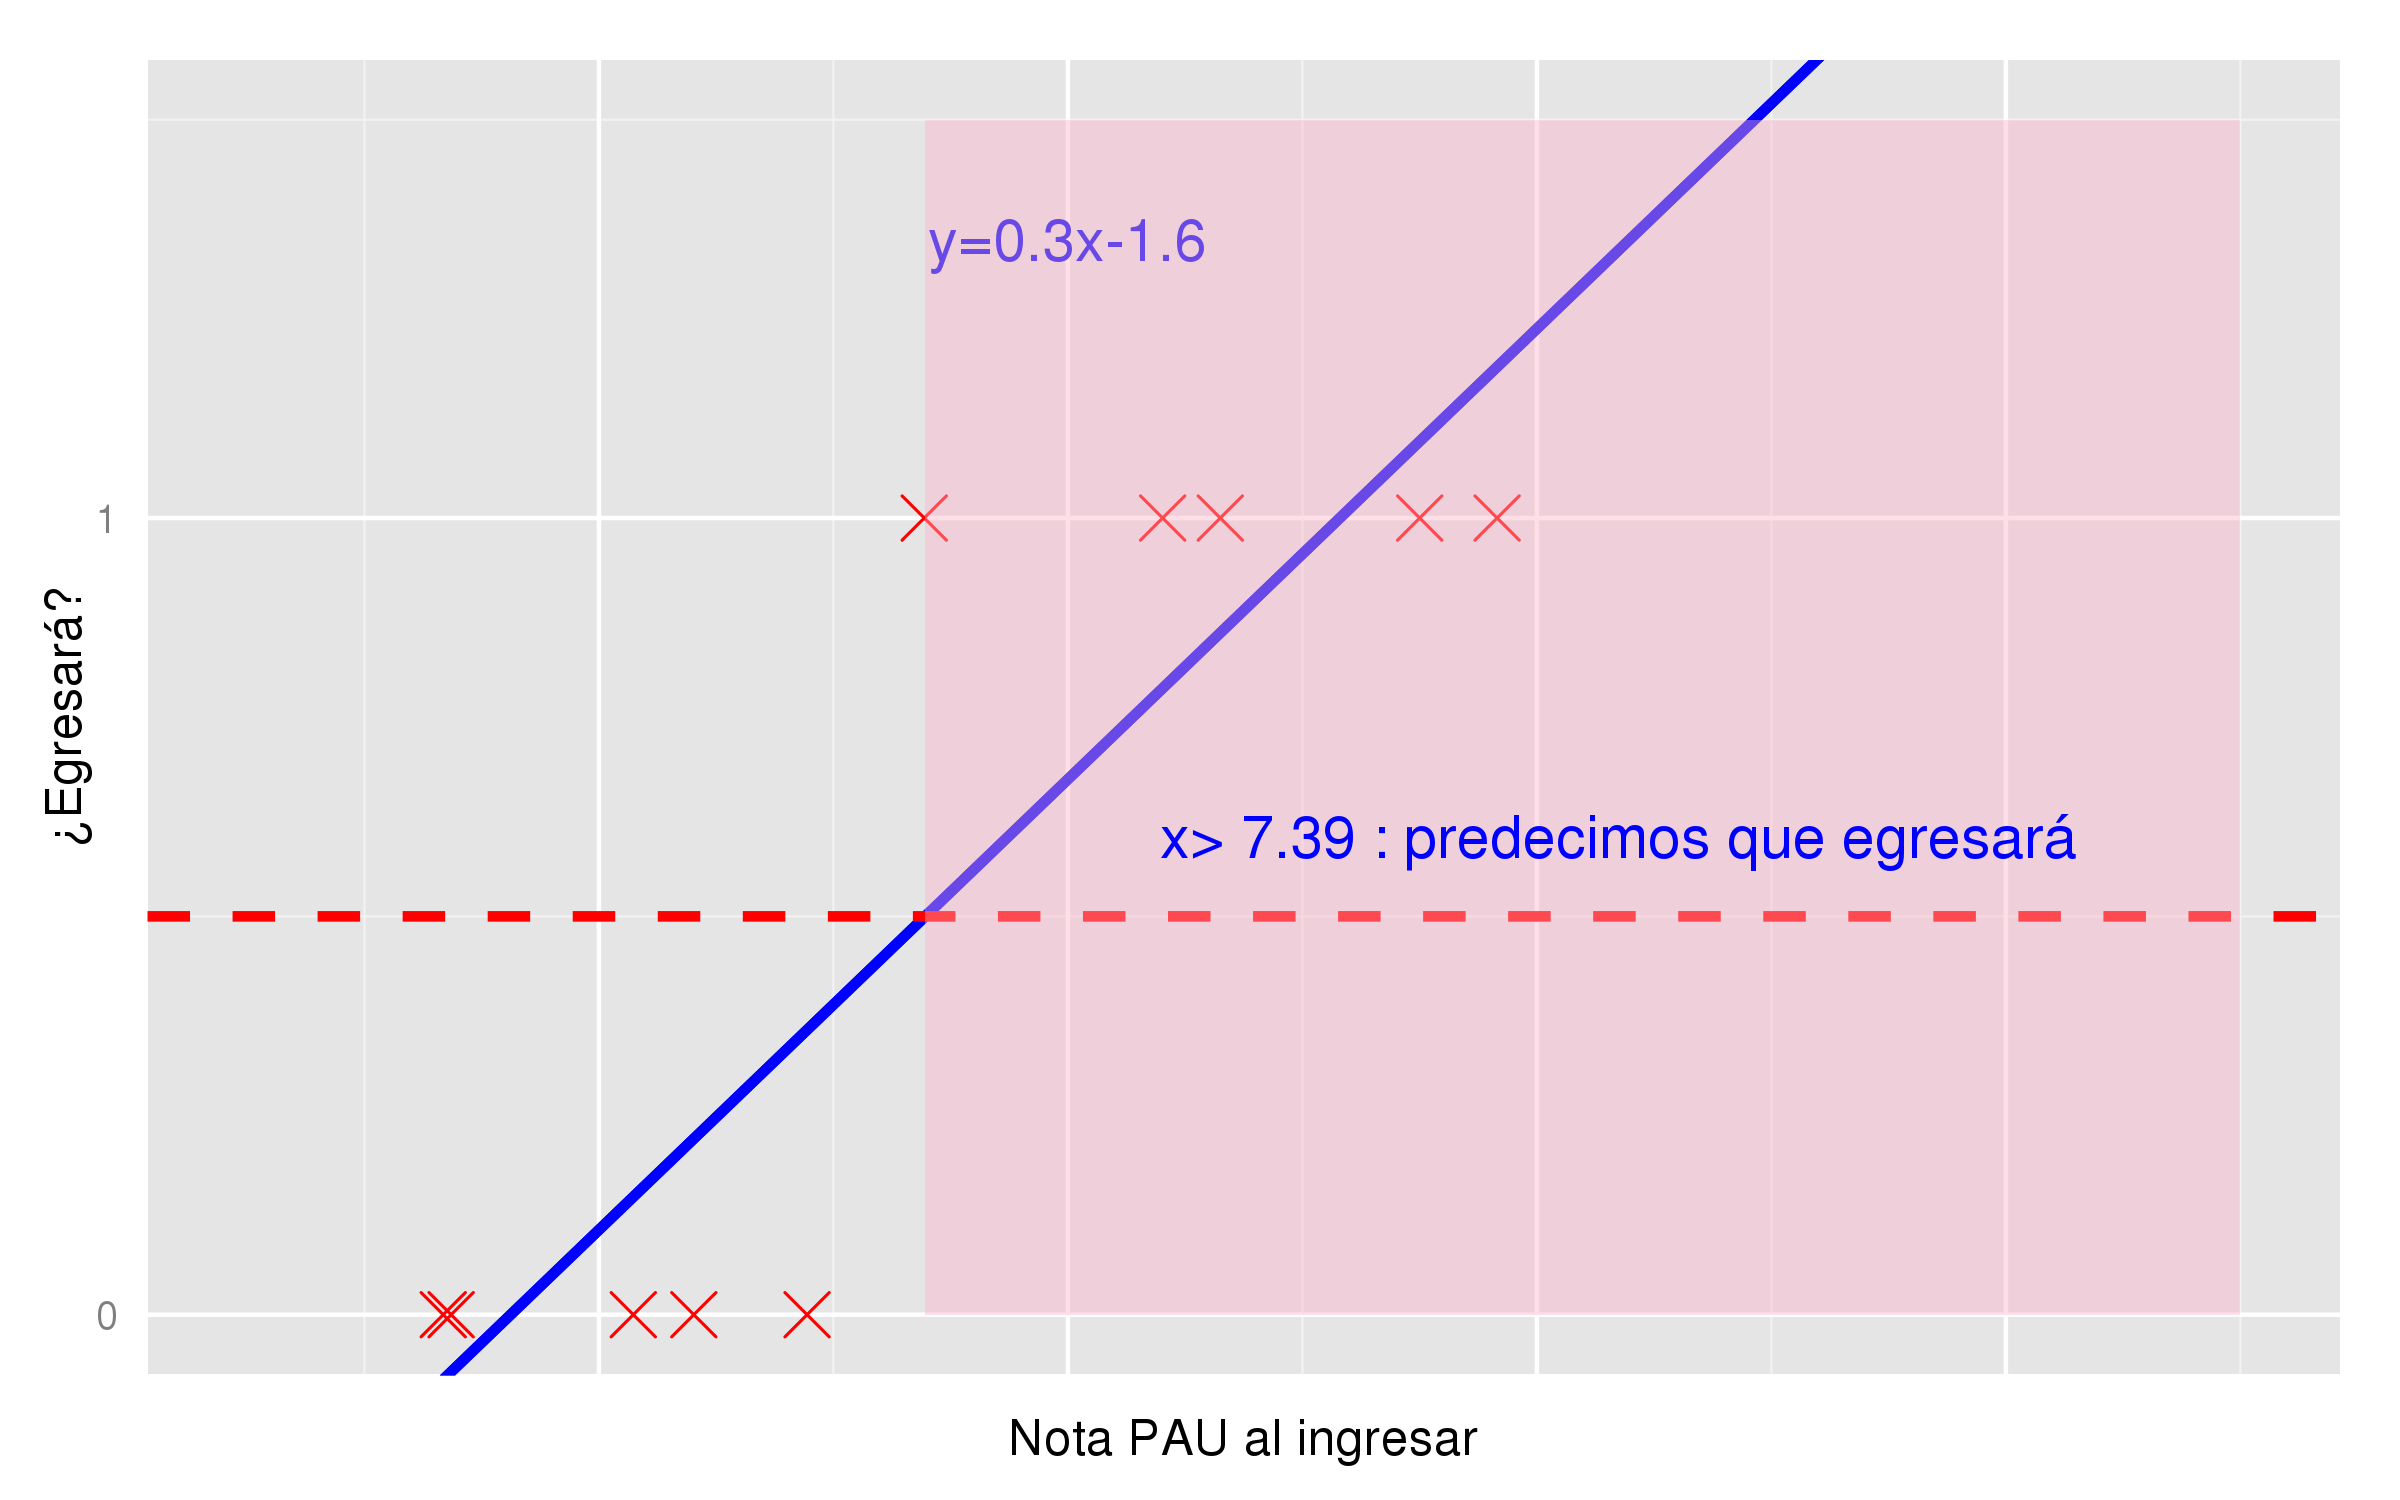
\includegraphics[height=6.6cm]{egresara8.png}
\end{center}
  \end{frame}
 \begin{frame}\frametitle{Ejemplo: predicción del abandono}
   \begin{overlayarea}{\textwidth}{\textheight} 
   Pero nuestro criterio de decisión es sensible a datos atípicos:
%% \begin{center}
%%   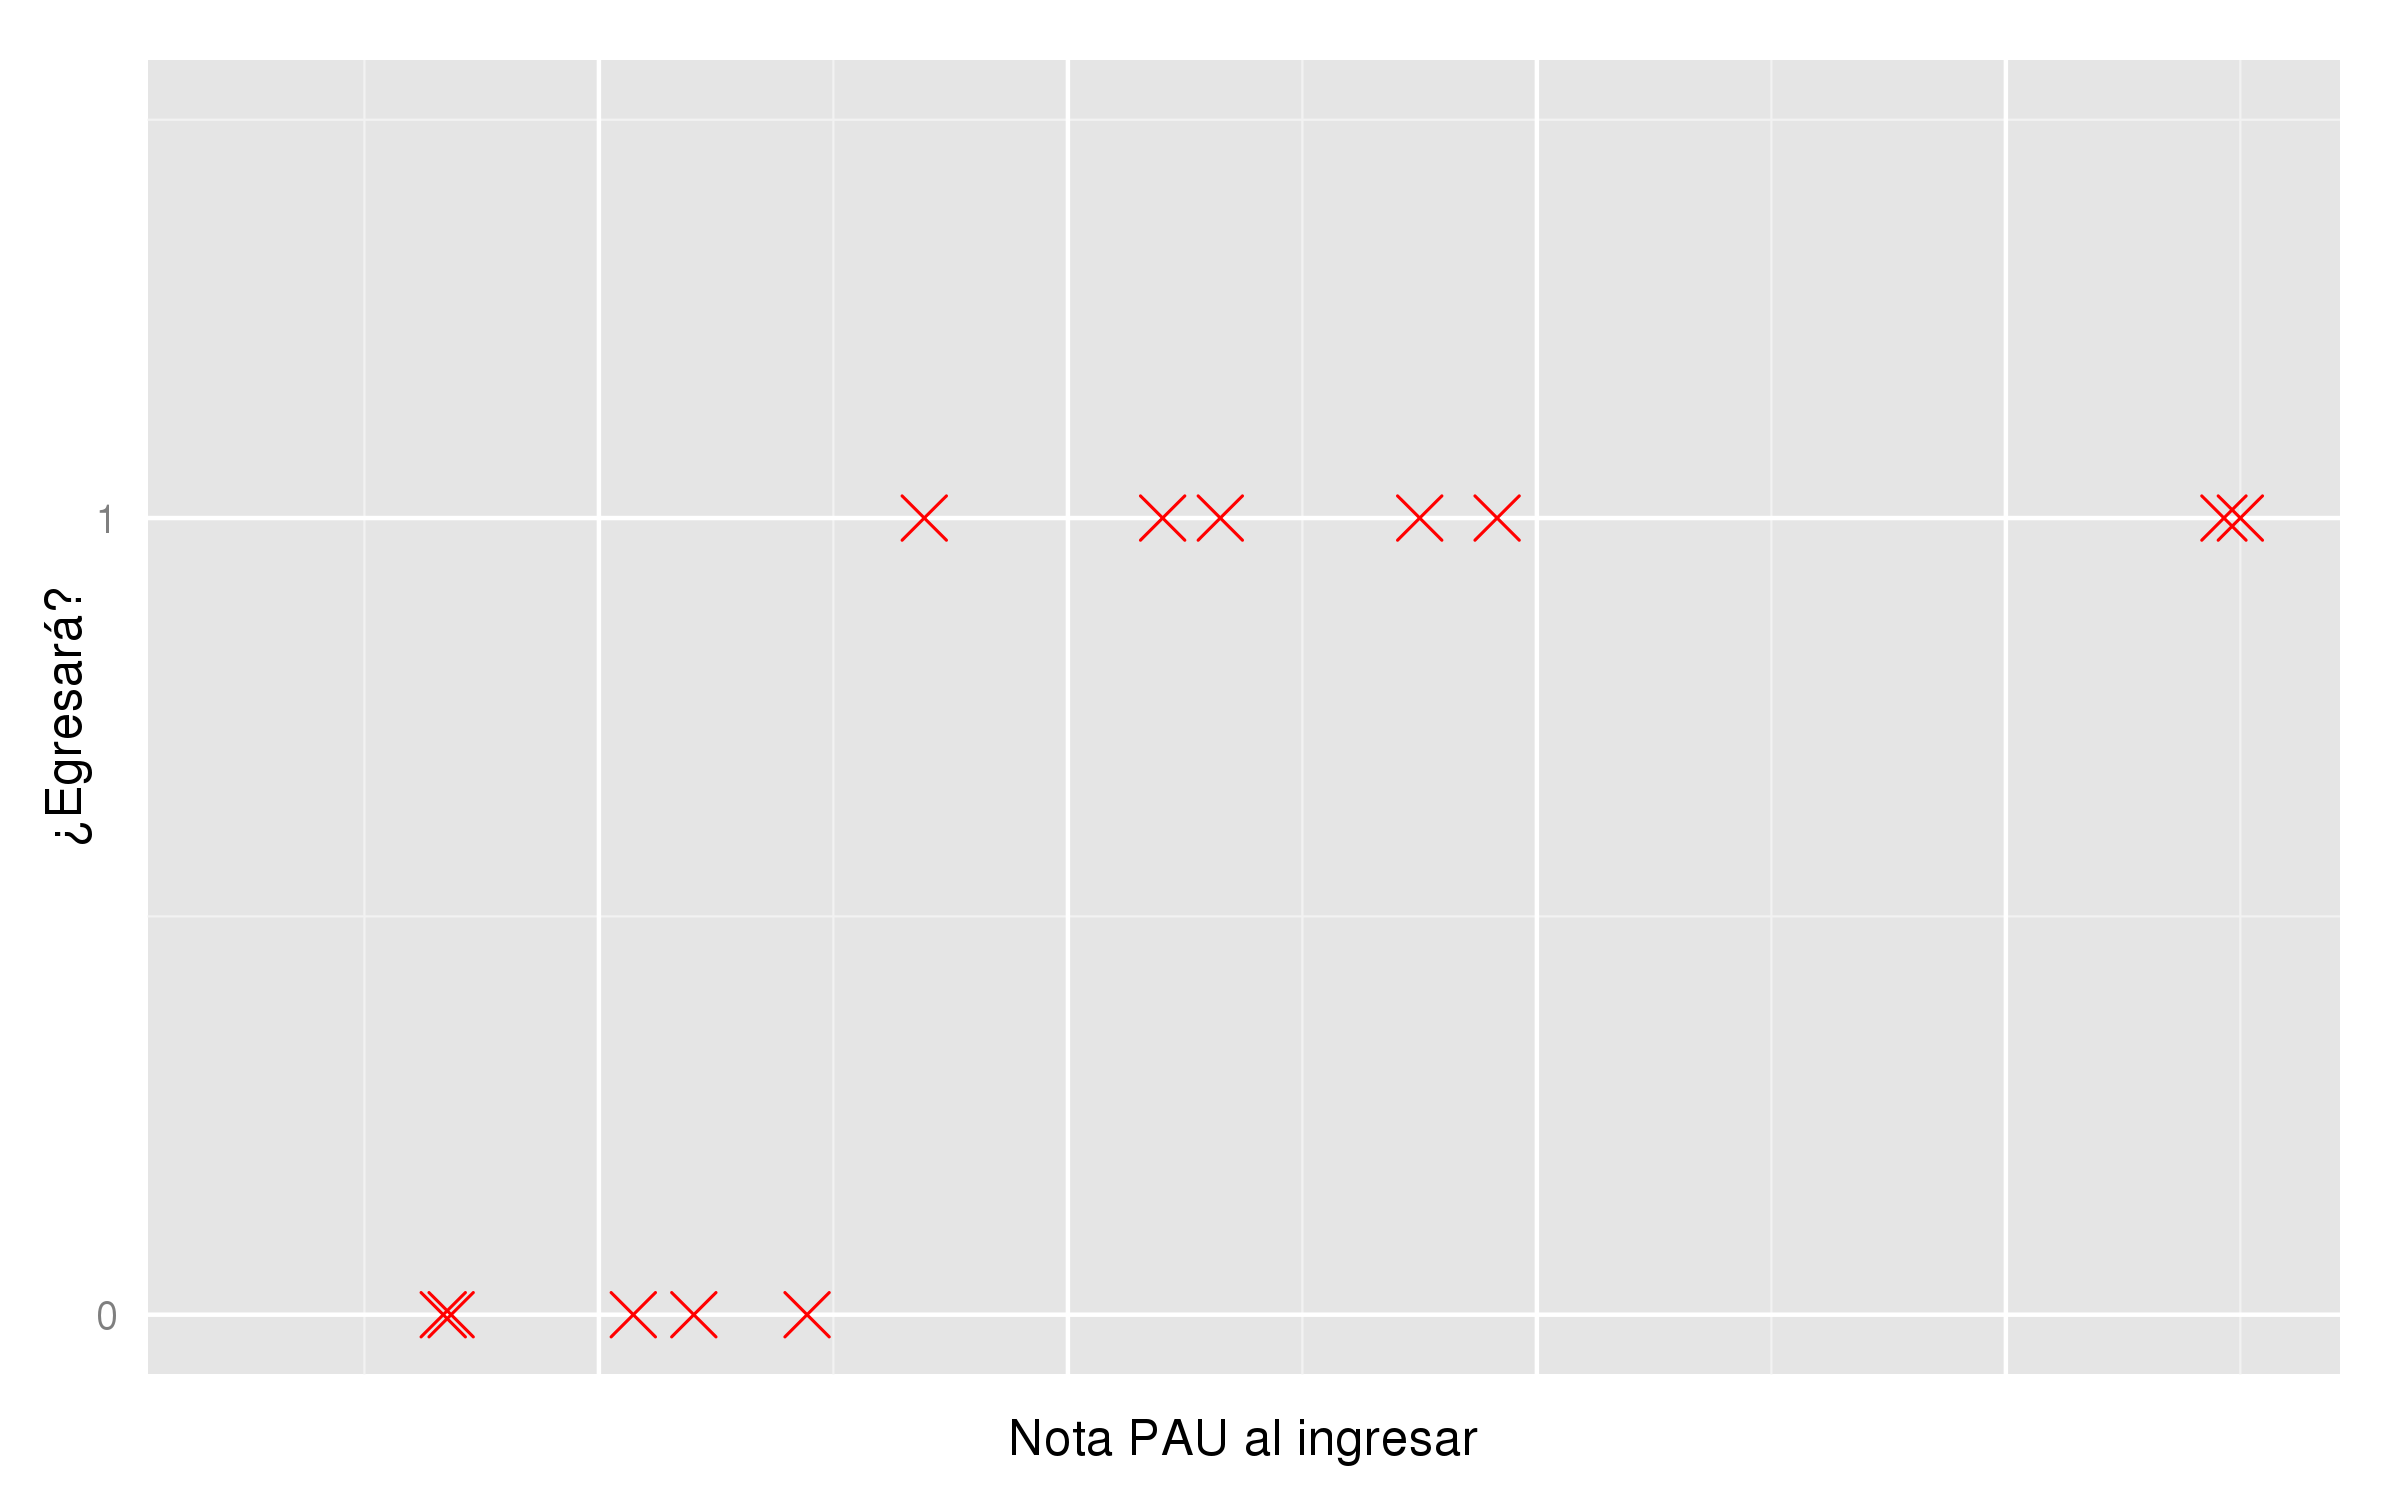
\includegraphics[height=6.6cm]{egresara9.png}
%% \end{center}
   \end{overlayarea}
 \end{frame}
 \begin{frame}\frametitle{Ejemplo: predicción del abandono}
   \begin{overlayarea}{\textwidth}{0.6cm} 
   Supongamos que tenemos estos puntos adicionales\onslide<2->
   \end{overlayarea}
\begin{center}
  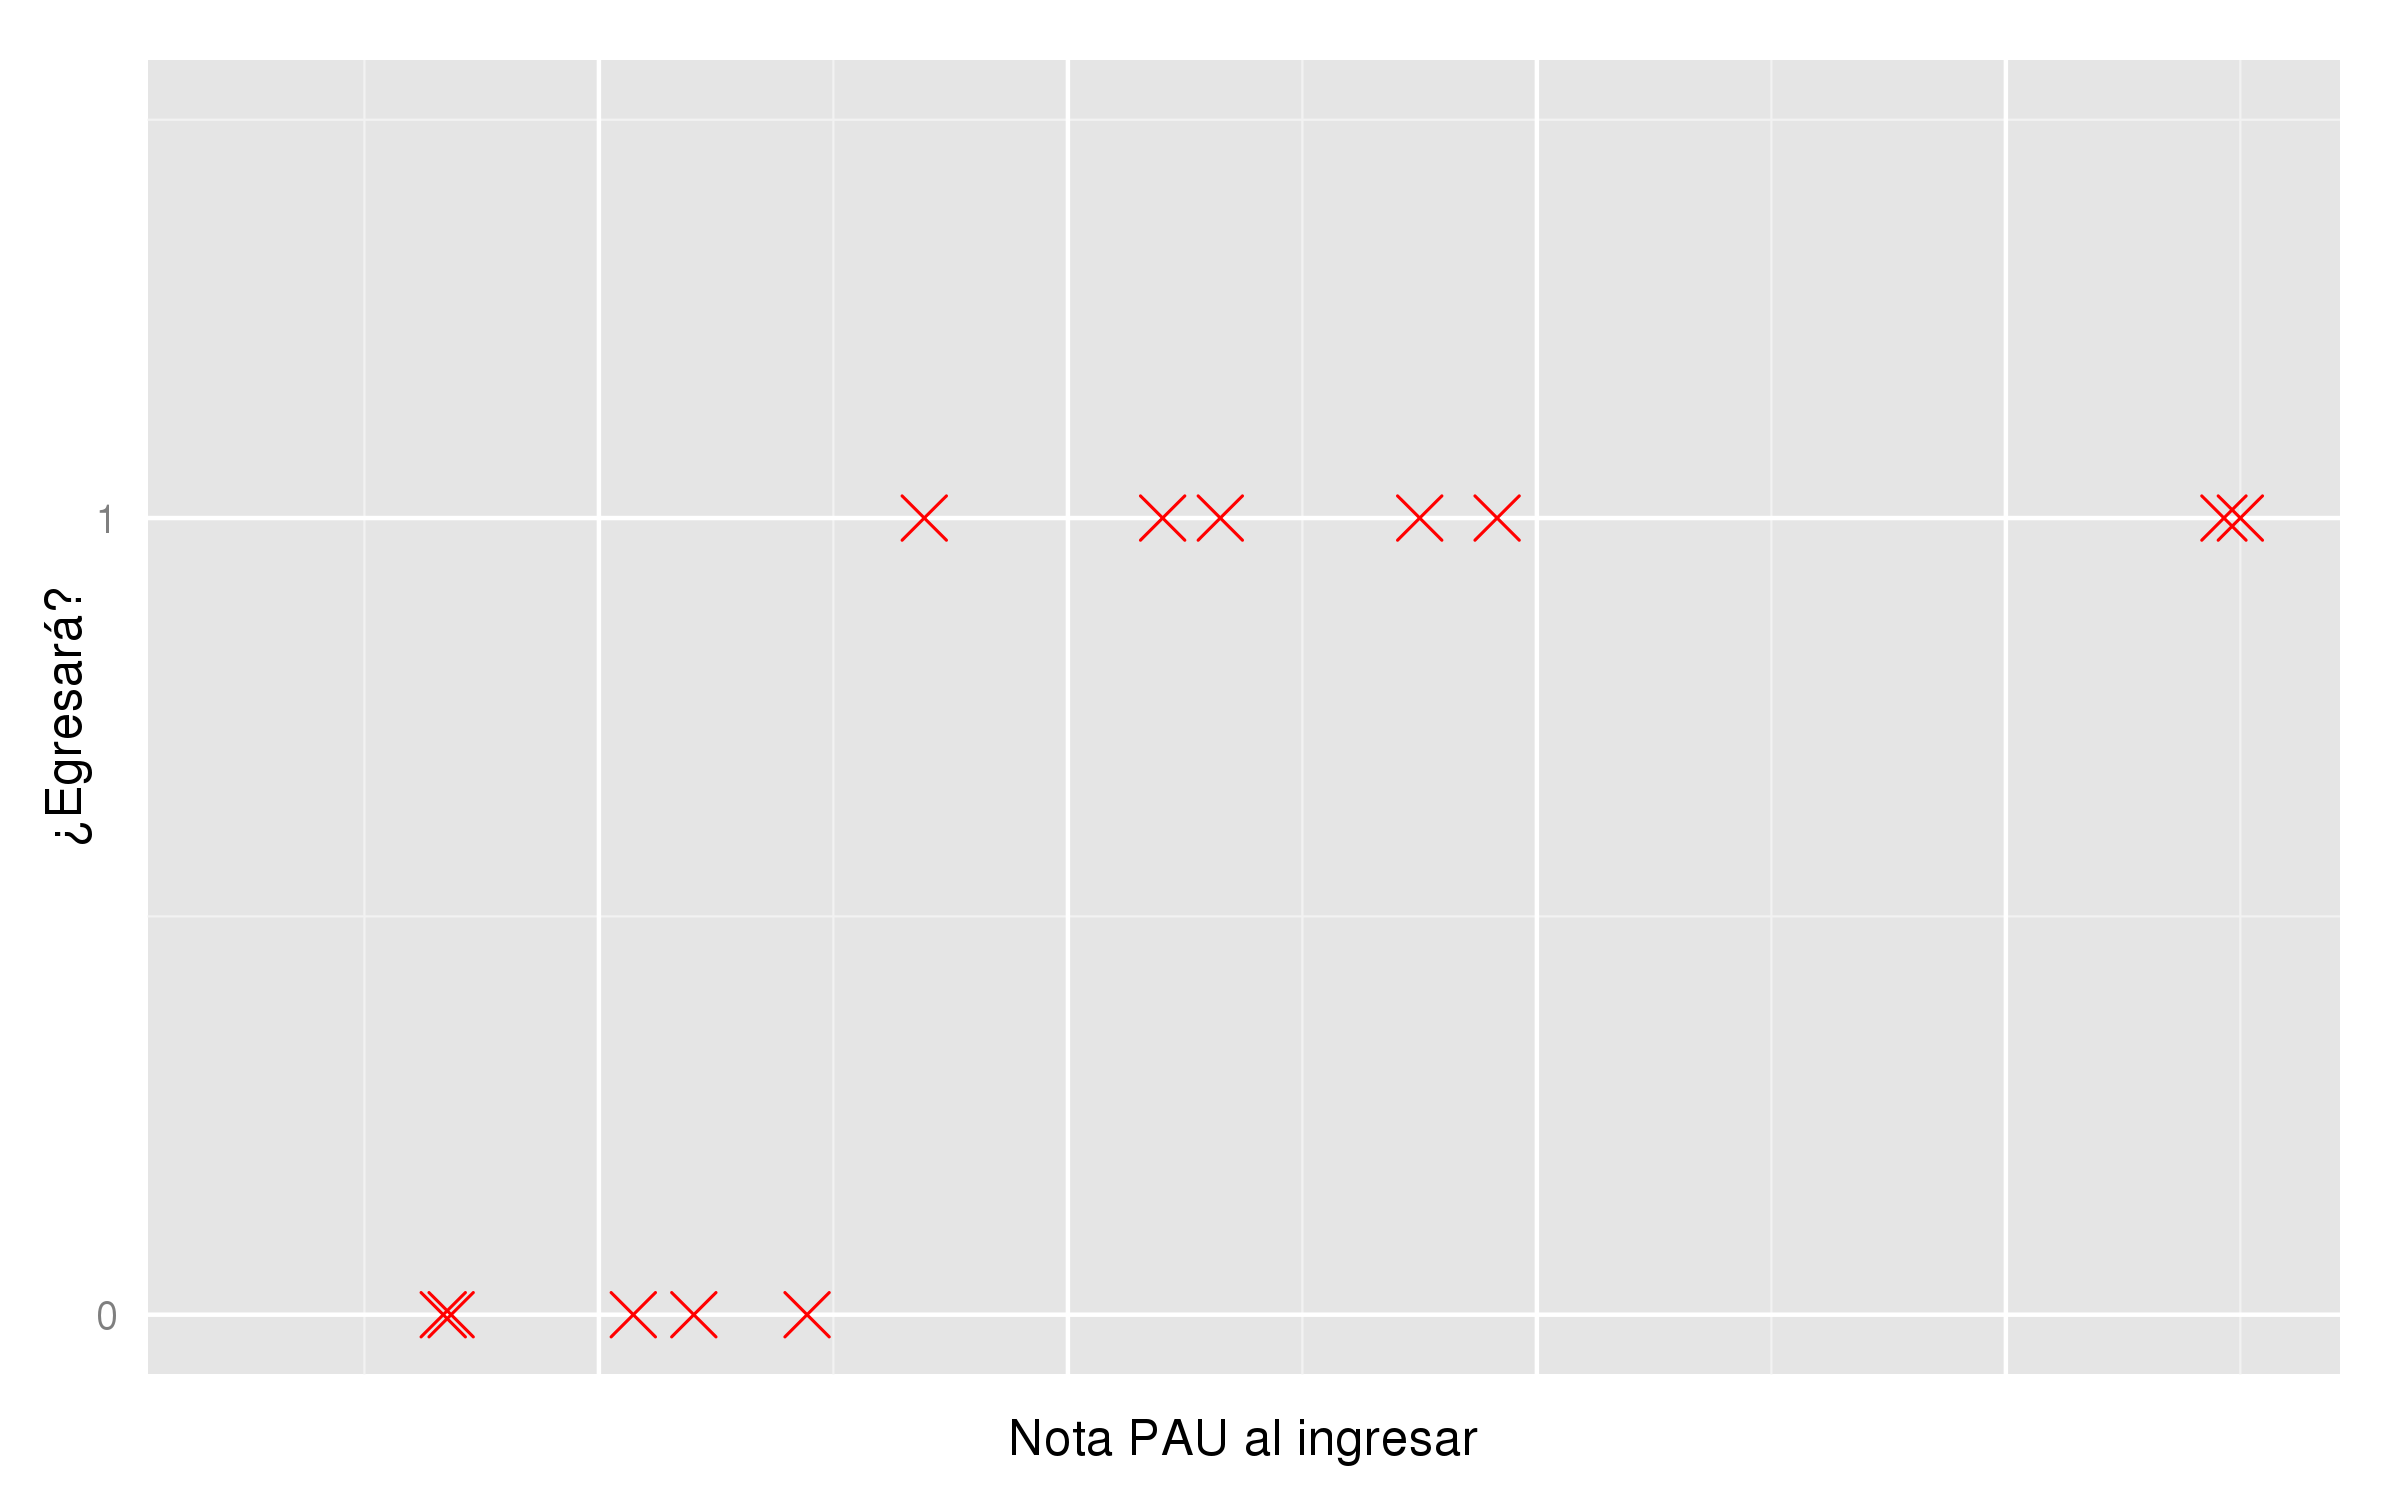
\includegraphics[height=6.6cm]{egresara9.png}
\end{center}
   
 \end{frame}
 
 \begin{frame}\frametitle{Ejemplo: predicción del abandono}
   \begin{overlayarea}{\textwidth}{0.6cm} 
   El ajuste cambia bastante
   \end{overlayarea}
   \begin{center}
  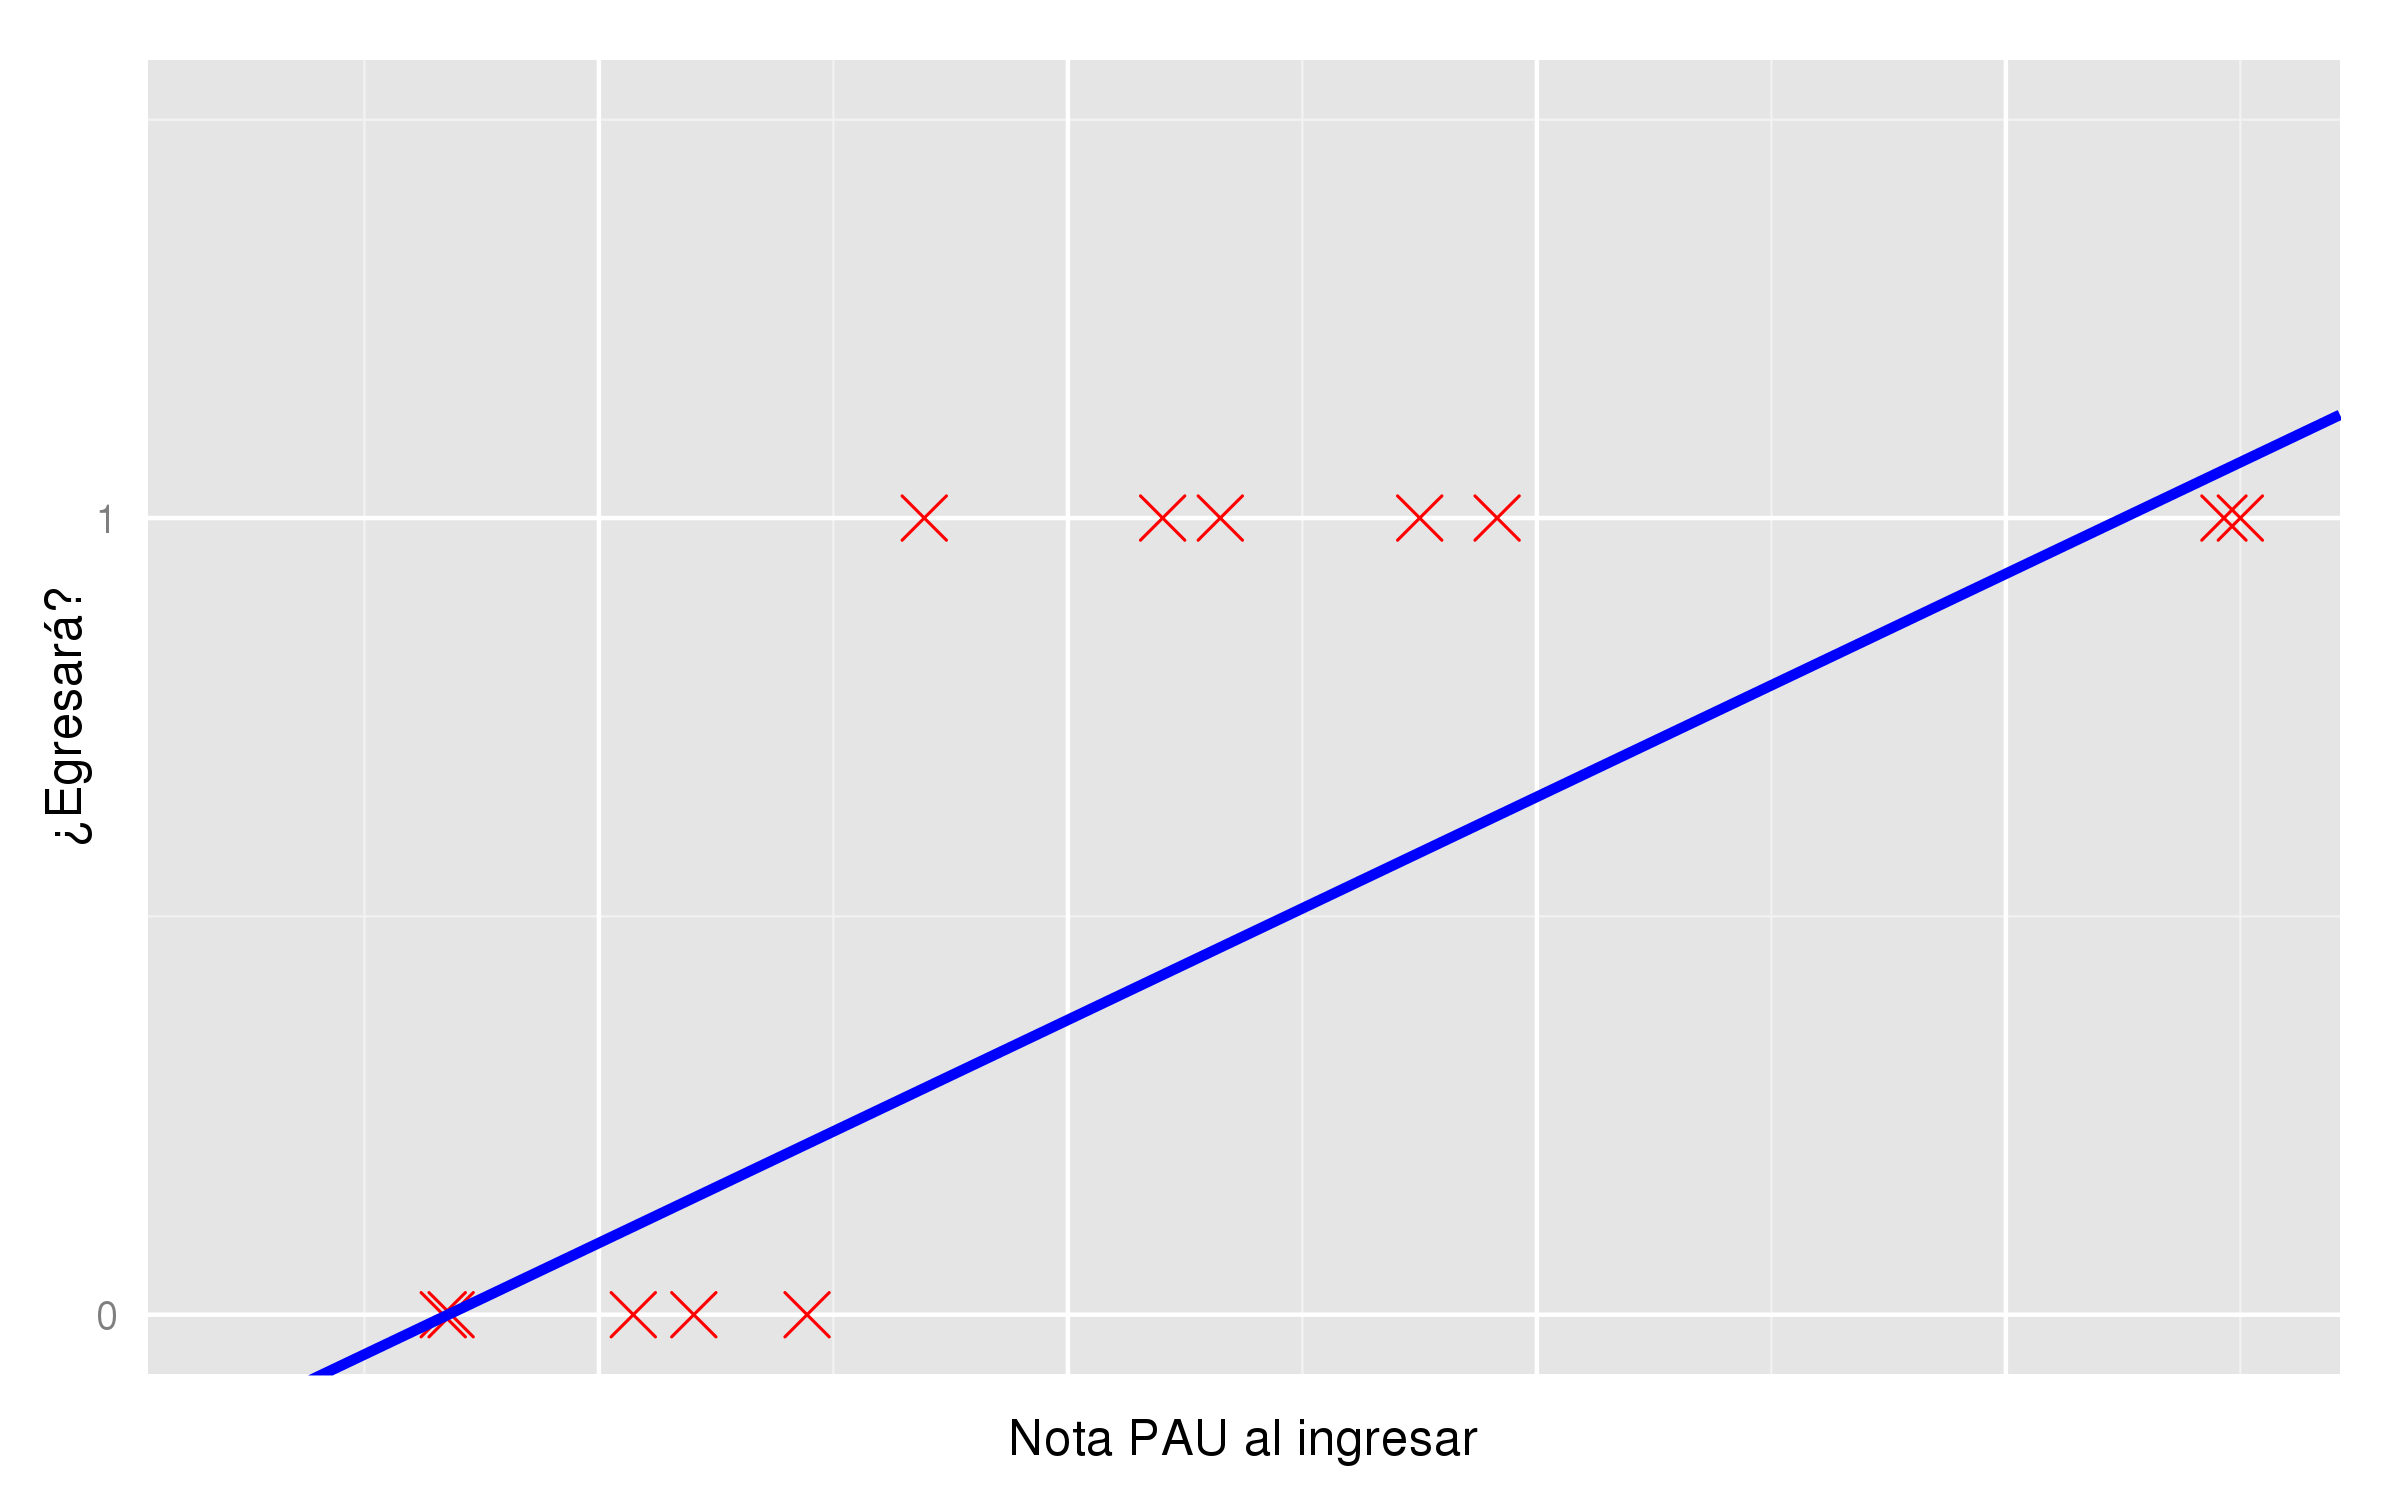
\includegraphics[height=6.6cm]{egresara10.png}
\end{center}

 \end{frame}
 \begin{frame}\frametitle{Ejemplo: predicción del abandono}
   \begin{overlayarea}{\textwidth}{0.6cm} 
   Y nuestro criterio de decisión es inadecuado
   \end{overlayarea}
   \begin{center}
  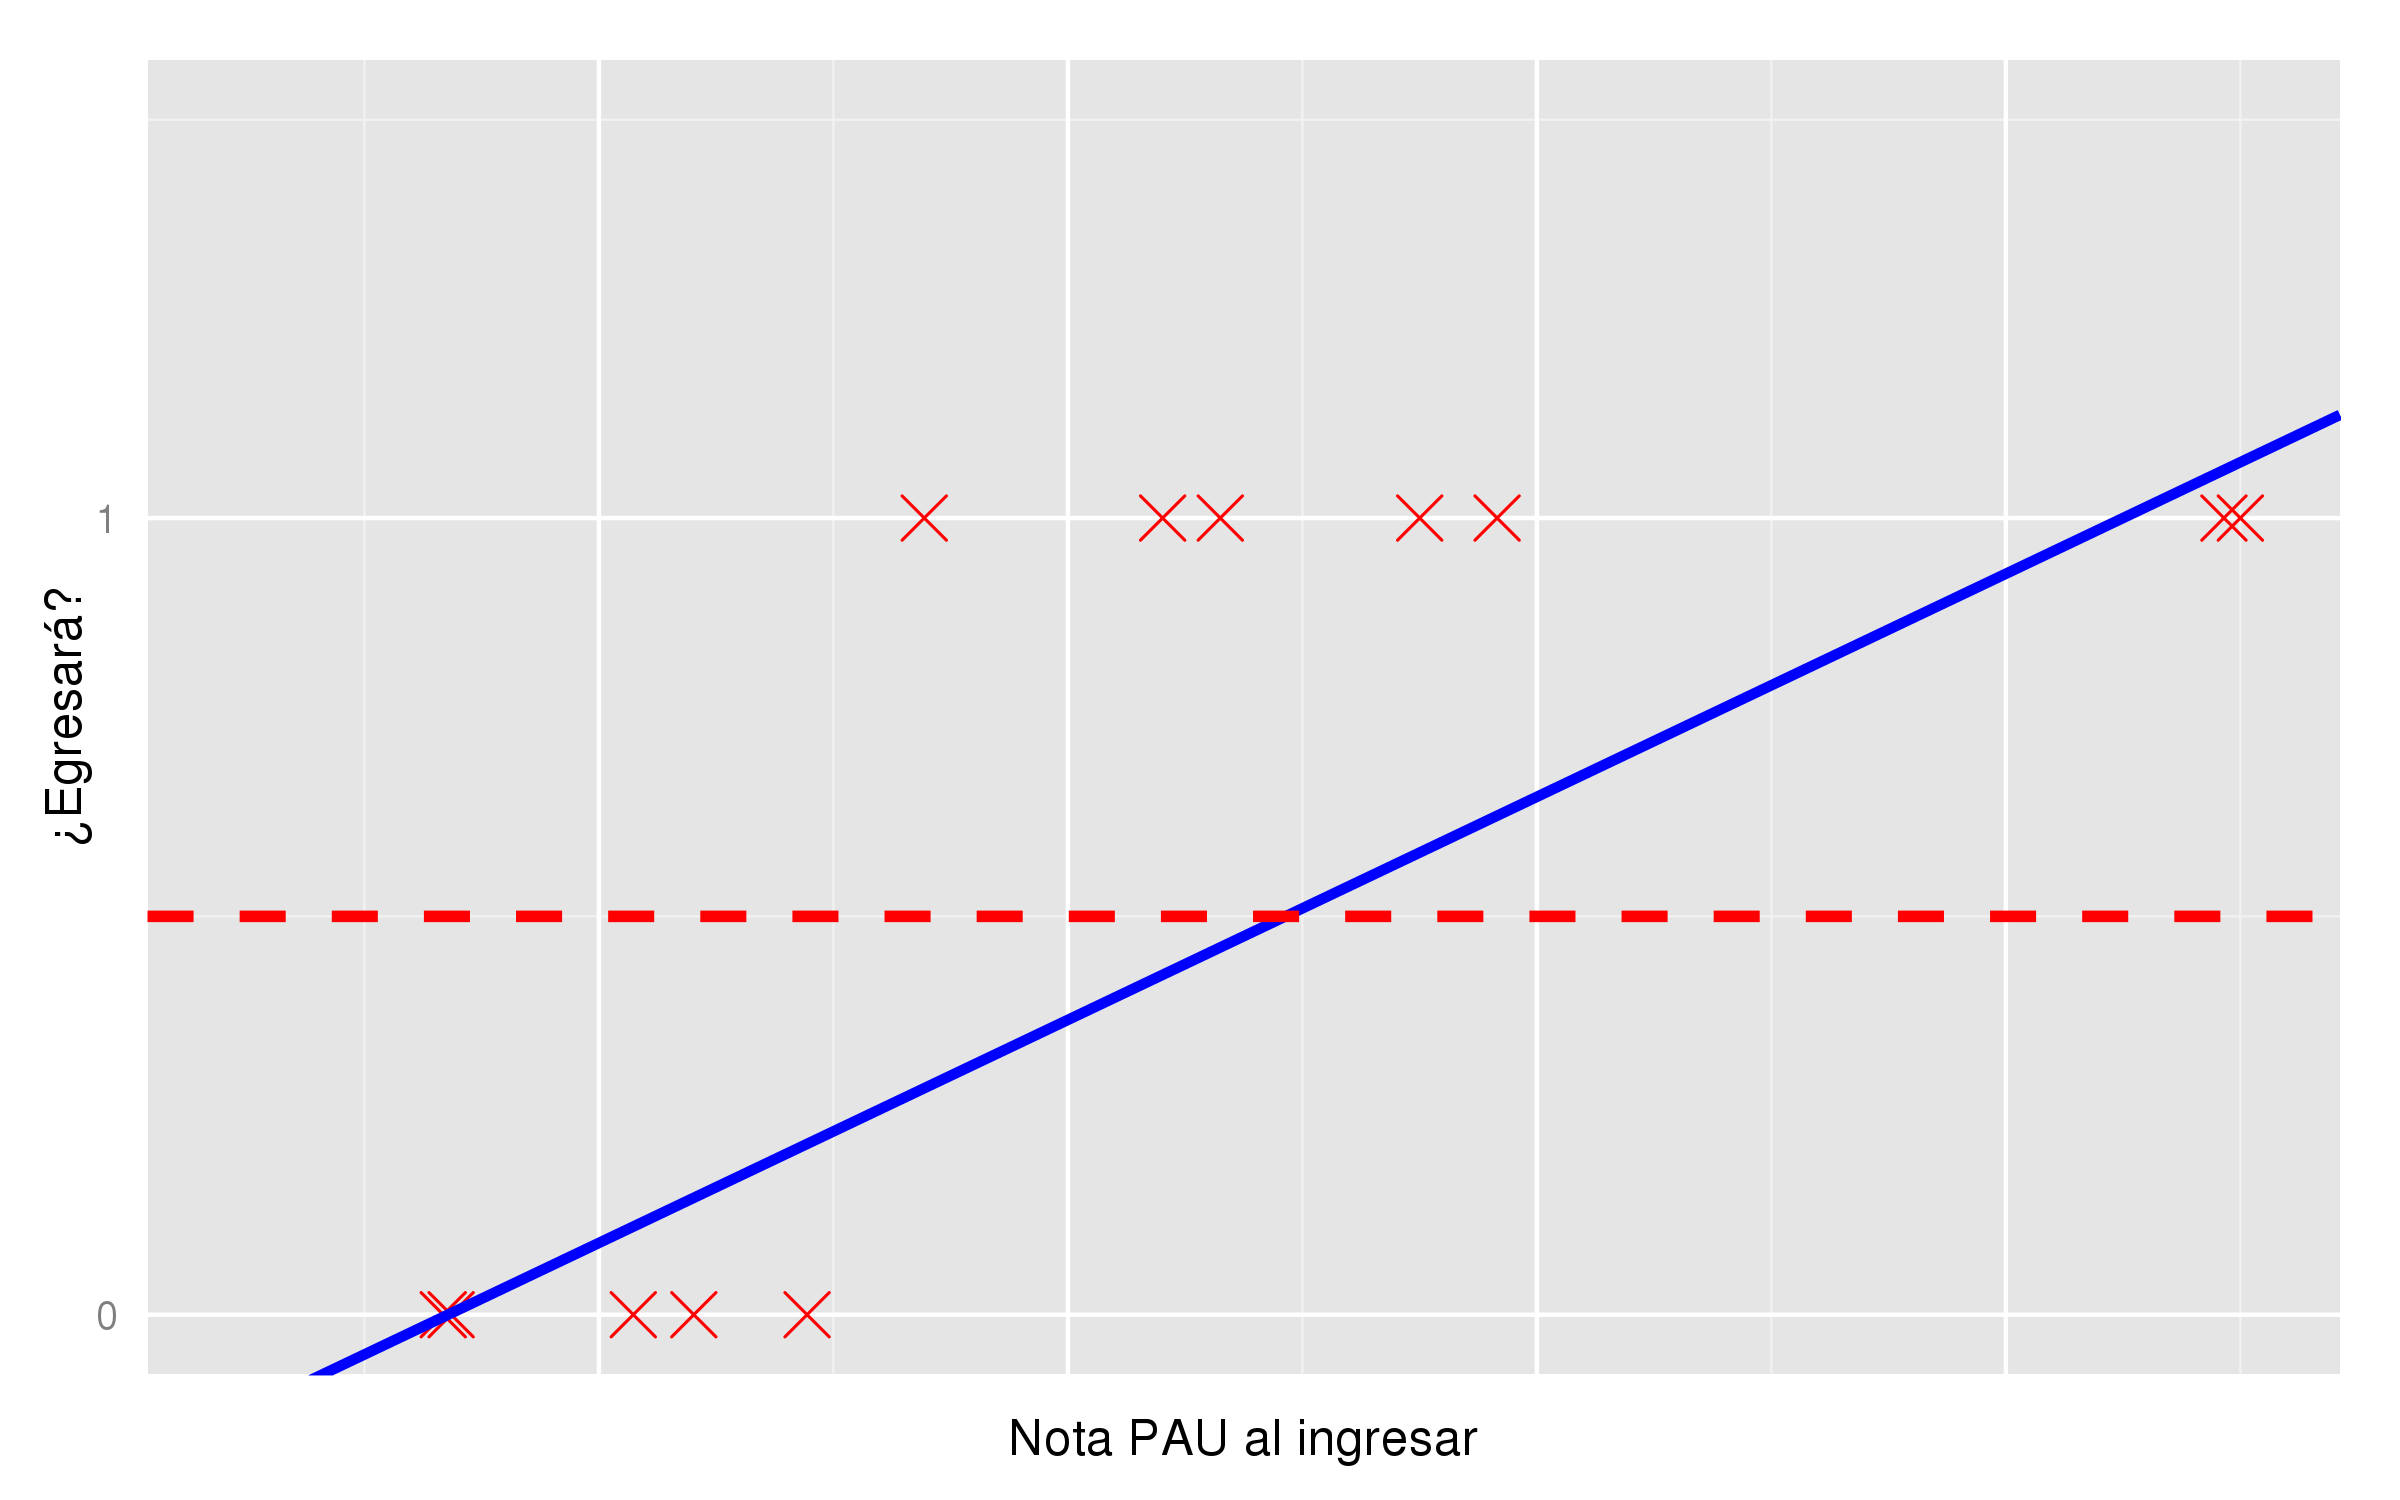
\includegraphics[height=6.6cm]{egresara11.png}
\end{center}

 \end{frame}
 \begin{frame}\frametitle{Ejemplo: predicción del abandono}
   \begin{overlayarea}{\textwidth}{0.6cm} 
   Y nuestro criterio de decisión es inadecuado
   \end{overlayarea}
   \begin{center}
  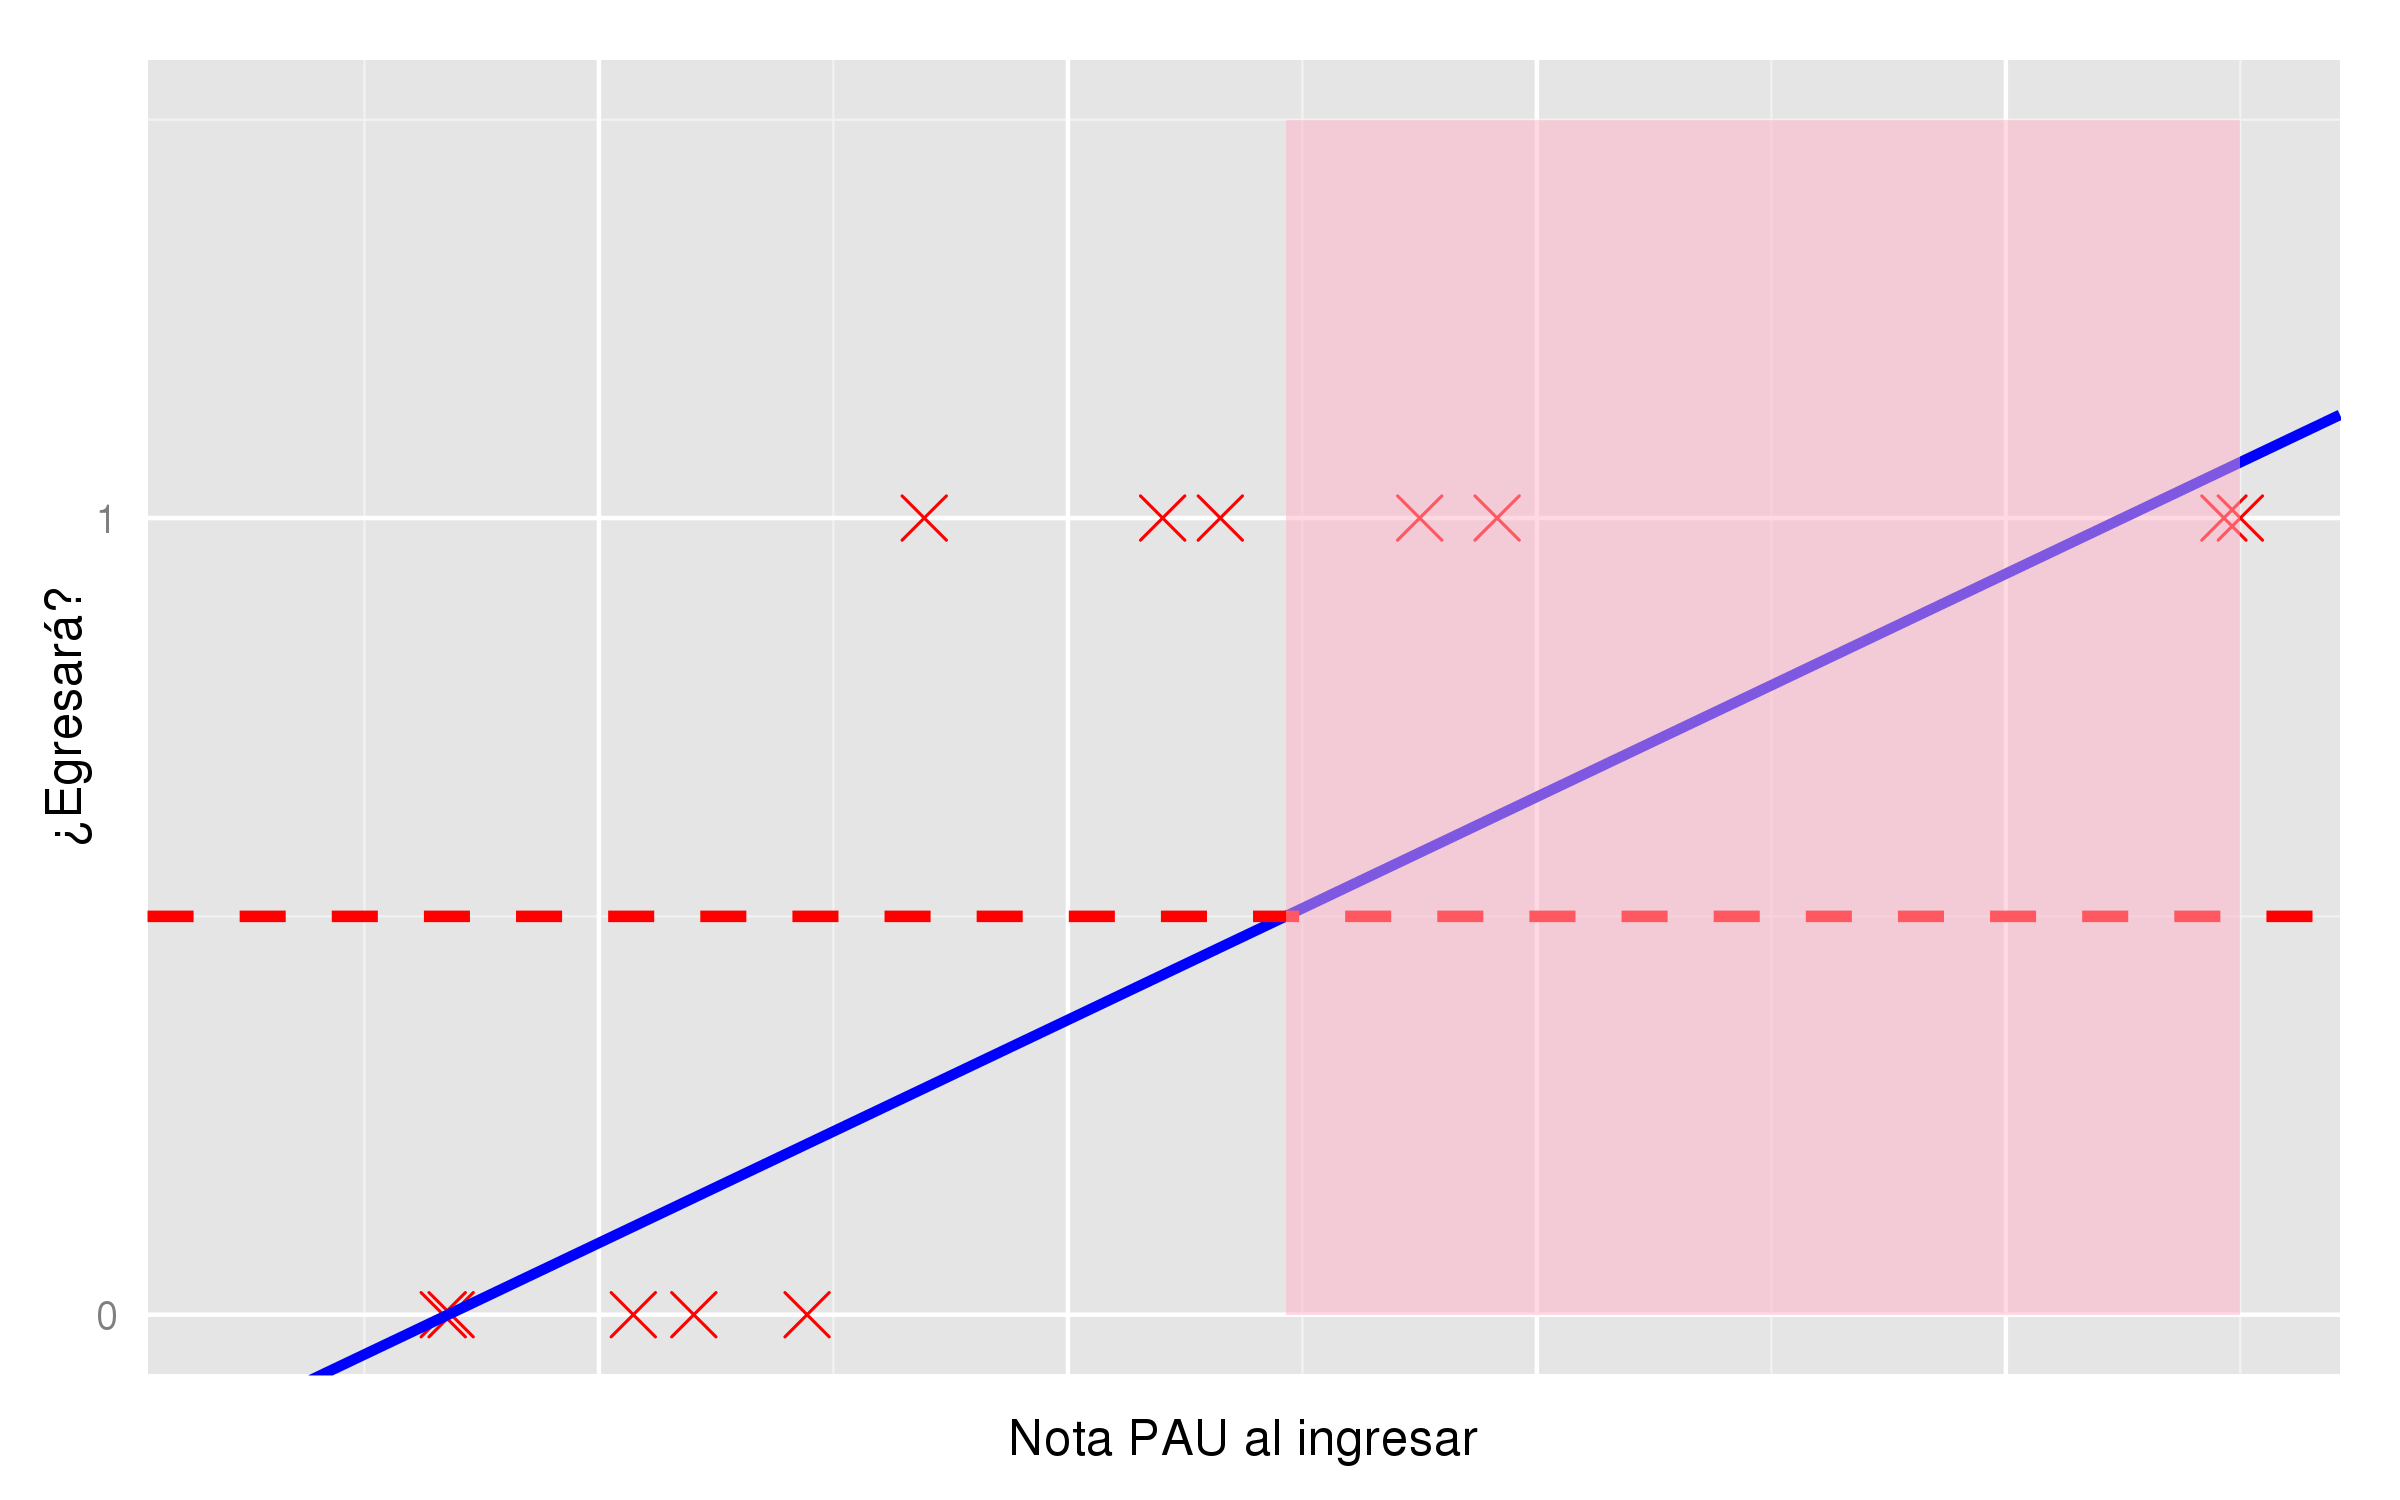
\includegraphics[height=6.6cm]{egresara12.png}
\end{center}

 \end{frame}
    \section{Función logística}
 \begin{frame}\frametitle{Regresión logística}
   \begin{overlayarea}{\textwidth}{\textheight}  
   Además al ajustar una recta a nuestros datos binarios, el modelo $h_\theta(x)$ puede tomar valores superiores a 1, o negativos...
   \onslide<2->
   \begin{block}{Pasamos a una función no lineal para ajustar estos datos binarios:}
     Usaremos como base la función logística:
     $$g(z)=\frac 1 {1+e^{-z}}.$$\vspace{-0.5cm}\onslide<3->
     \begin{center}
  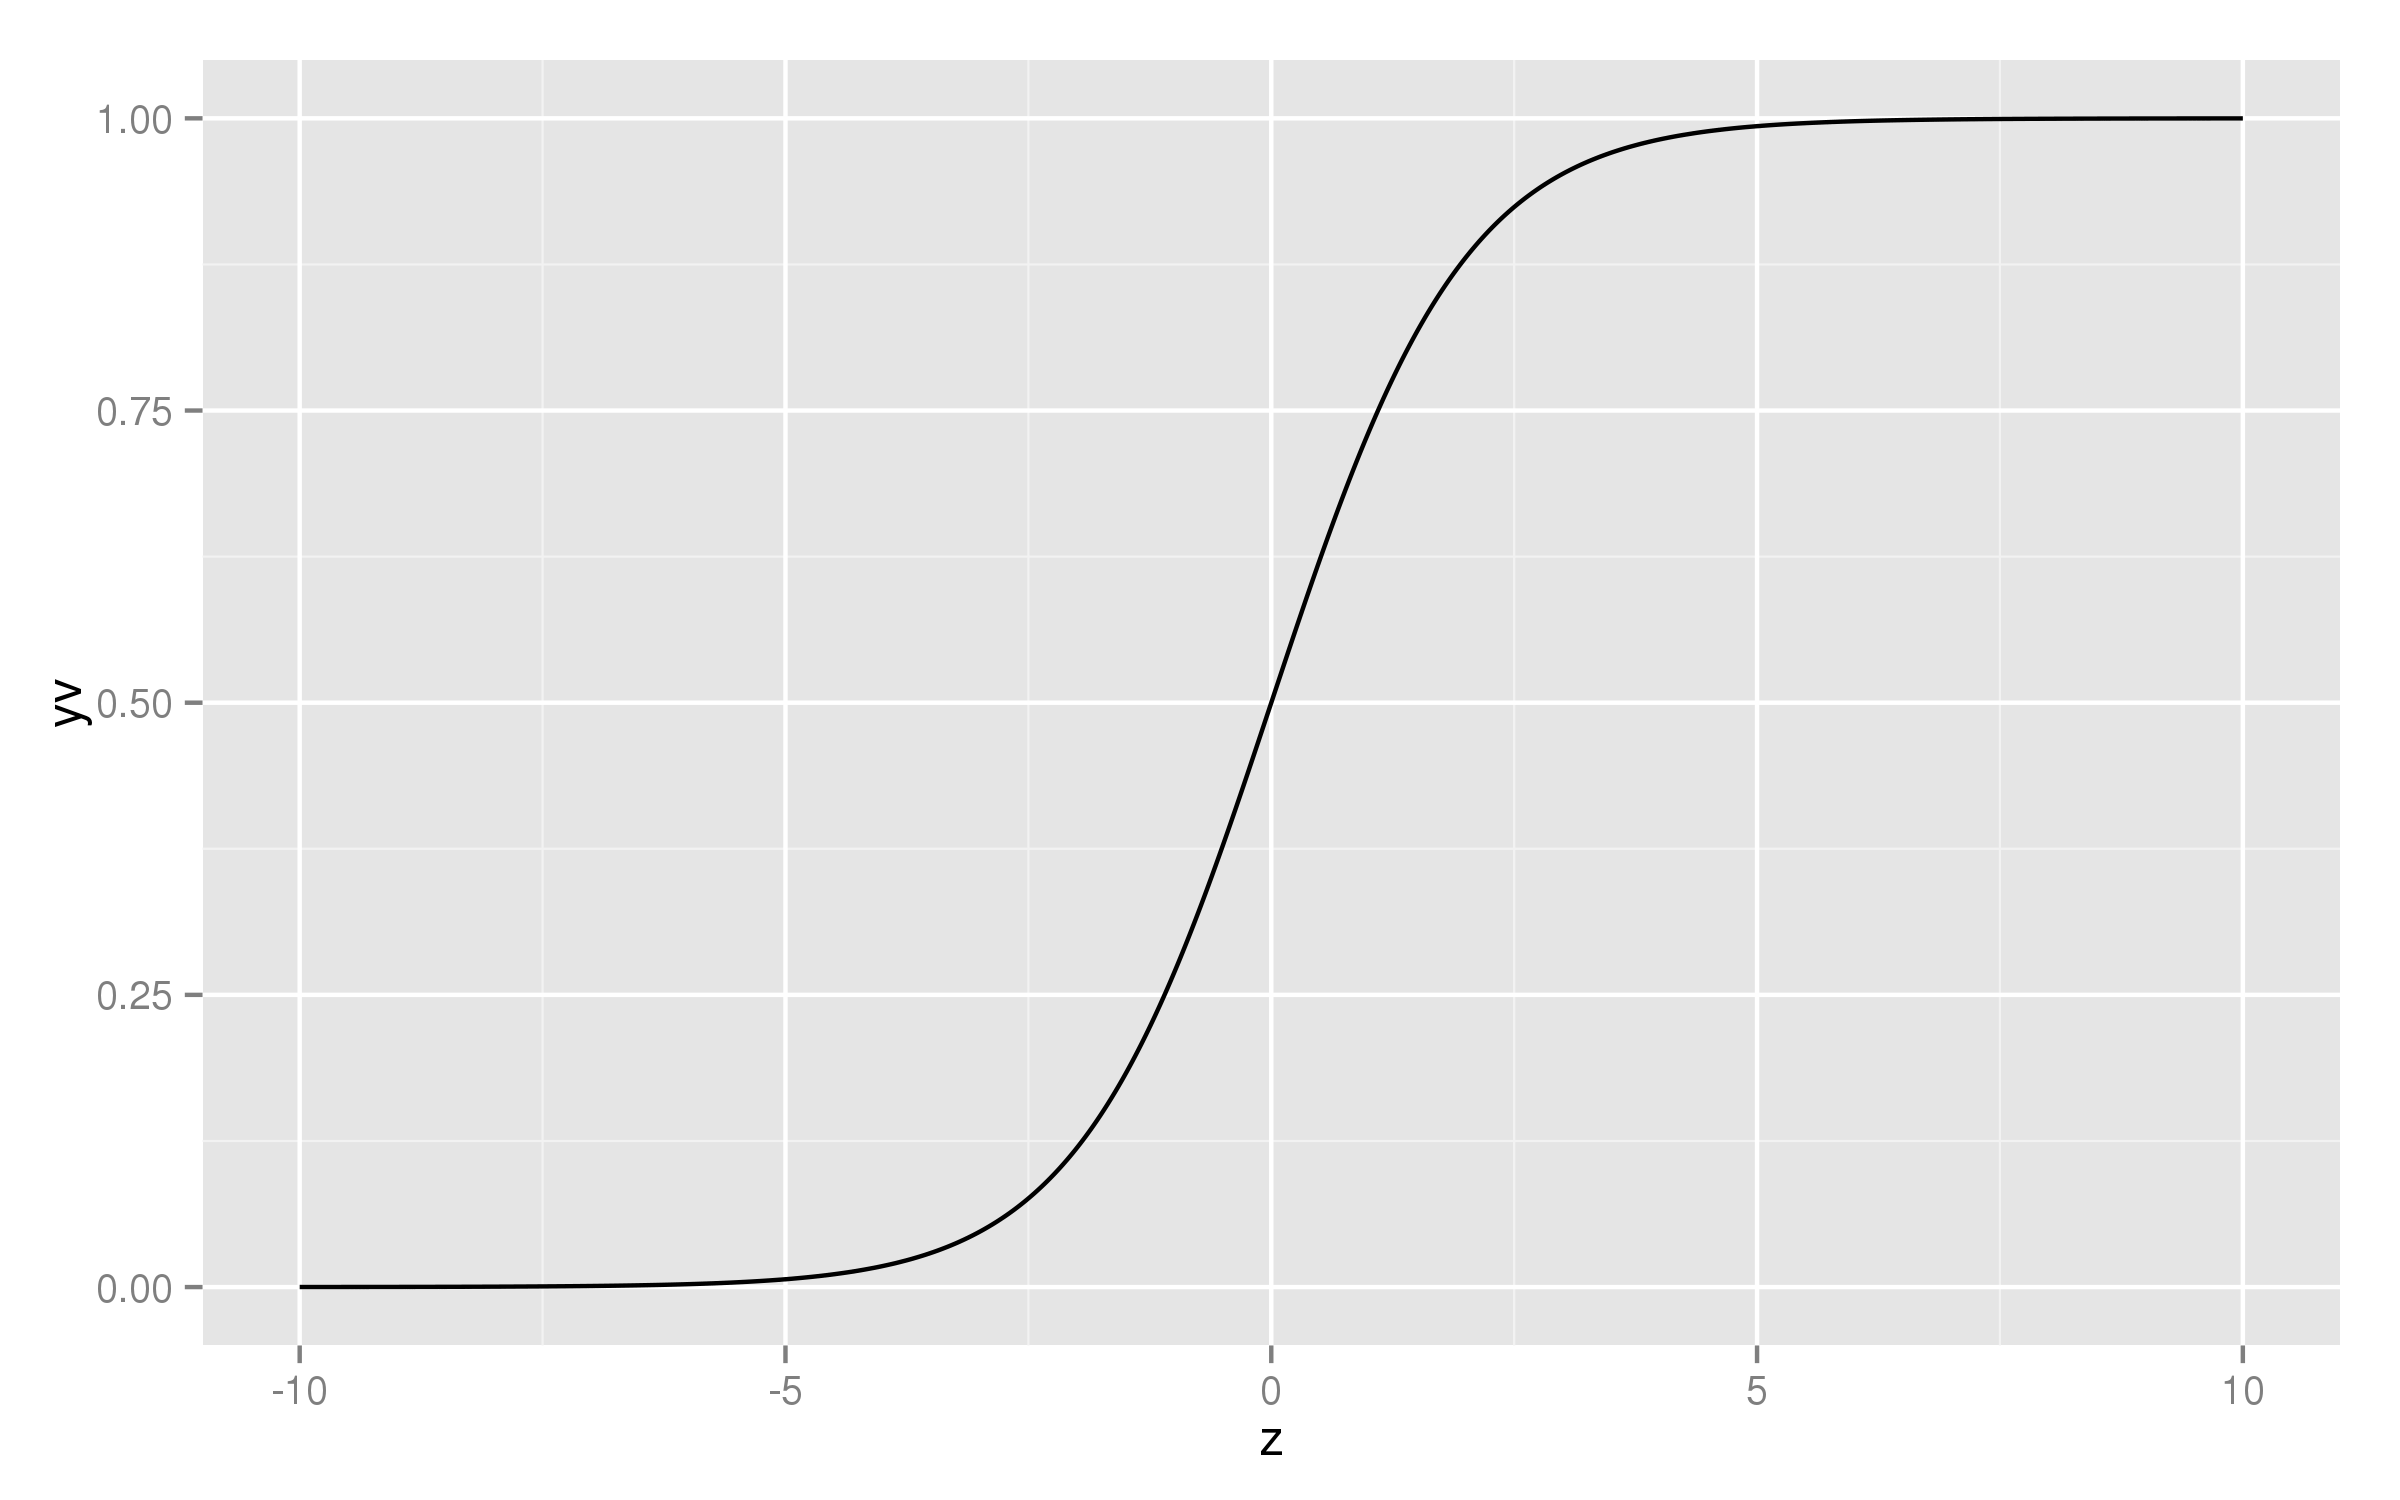
\includegraphics[height=3.6cm]{sigmoid.png}
\end{center}
   \end{block}
   \end{overlayarea}
   \end{frame}
   \section{El modelo para el ajuste}
 \begin{frame}\frametitle{Regresión logística}
   Ajustaremos a los datos binarios la hipótesis:        \begin{center}
          \fcolorbox{red}{white}{$\displaystyle h_\theta(x)=g(x^T\theta)$}
        \end{center}  

   \begin{enumerate}
   \item<2-> Si tenemos una única característica $x_1$:
        \begin{center}
          \fcolorbox{red}{white}{$\displaystyle h_\theta(x)=g(x^T\theta)=\frac 1 {1+e^{-(\theta_0+\theta_1x_1)}},$}
        \end{center}  
      \item<3->  si tenemos $k$ características $x_1,x_2,\ldots,x_k$. 
        \begin{center}
          \fcolorbox{red}{white}{$\displaystyle h_\theta(x)=g(x^T\theta)=\frac 1 {1+e^{-(\theta_0+\theta_1x_1+\ldots +\theta_kx_k)}},$}
        \end{center}  
   \end{enumerate}
   \end{frame}
 
 \begin{frame}\frametitle{En el caso de una característica, efecto de variar $\theta$}
 \begin{center} 
  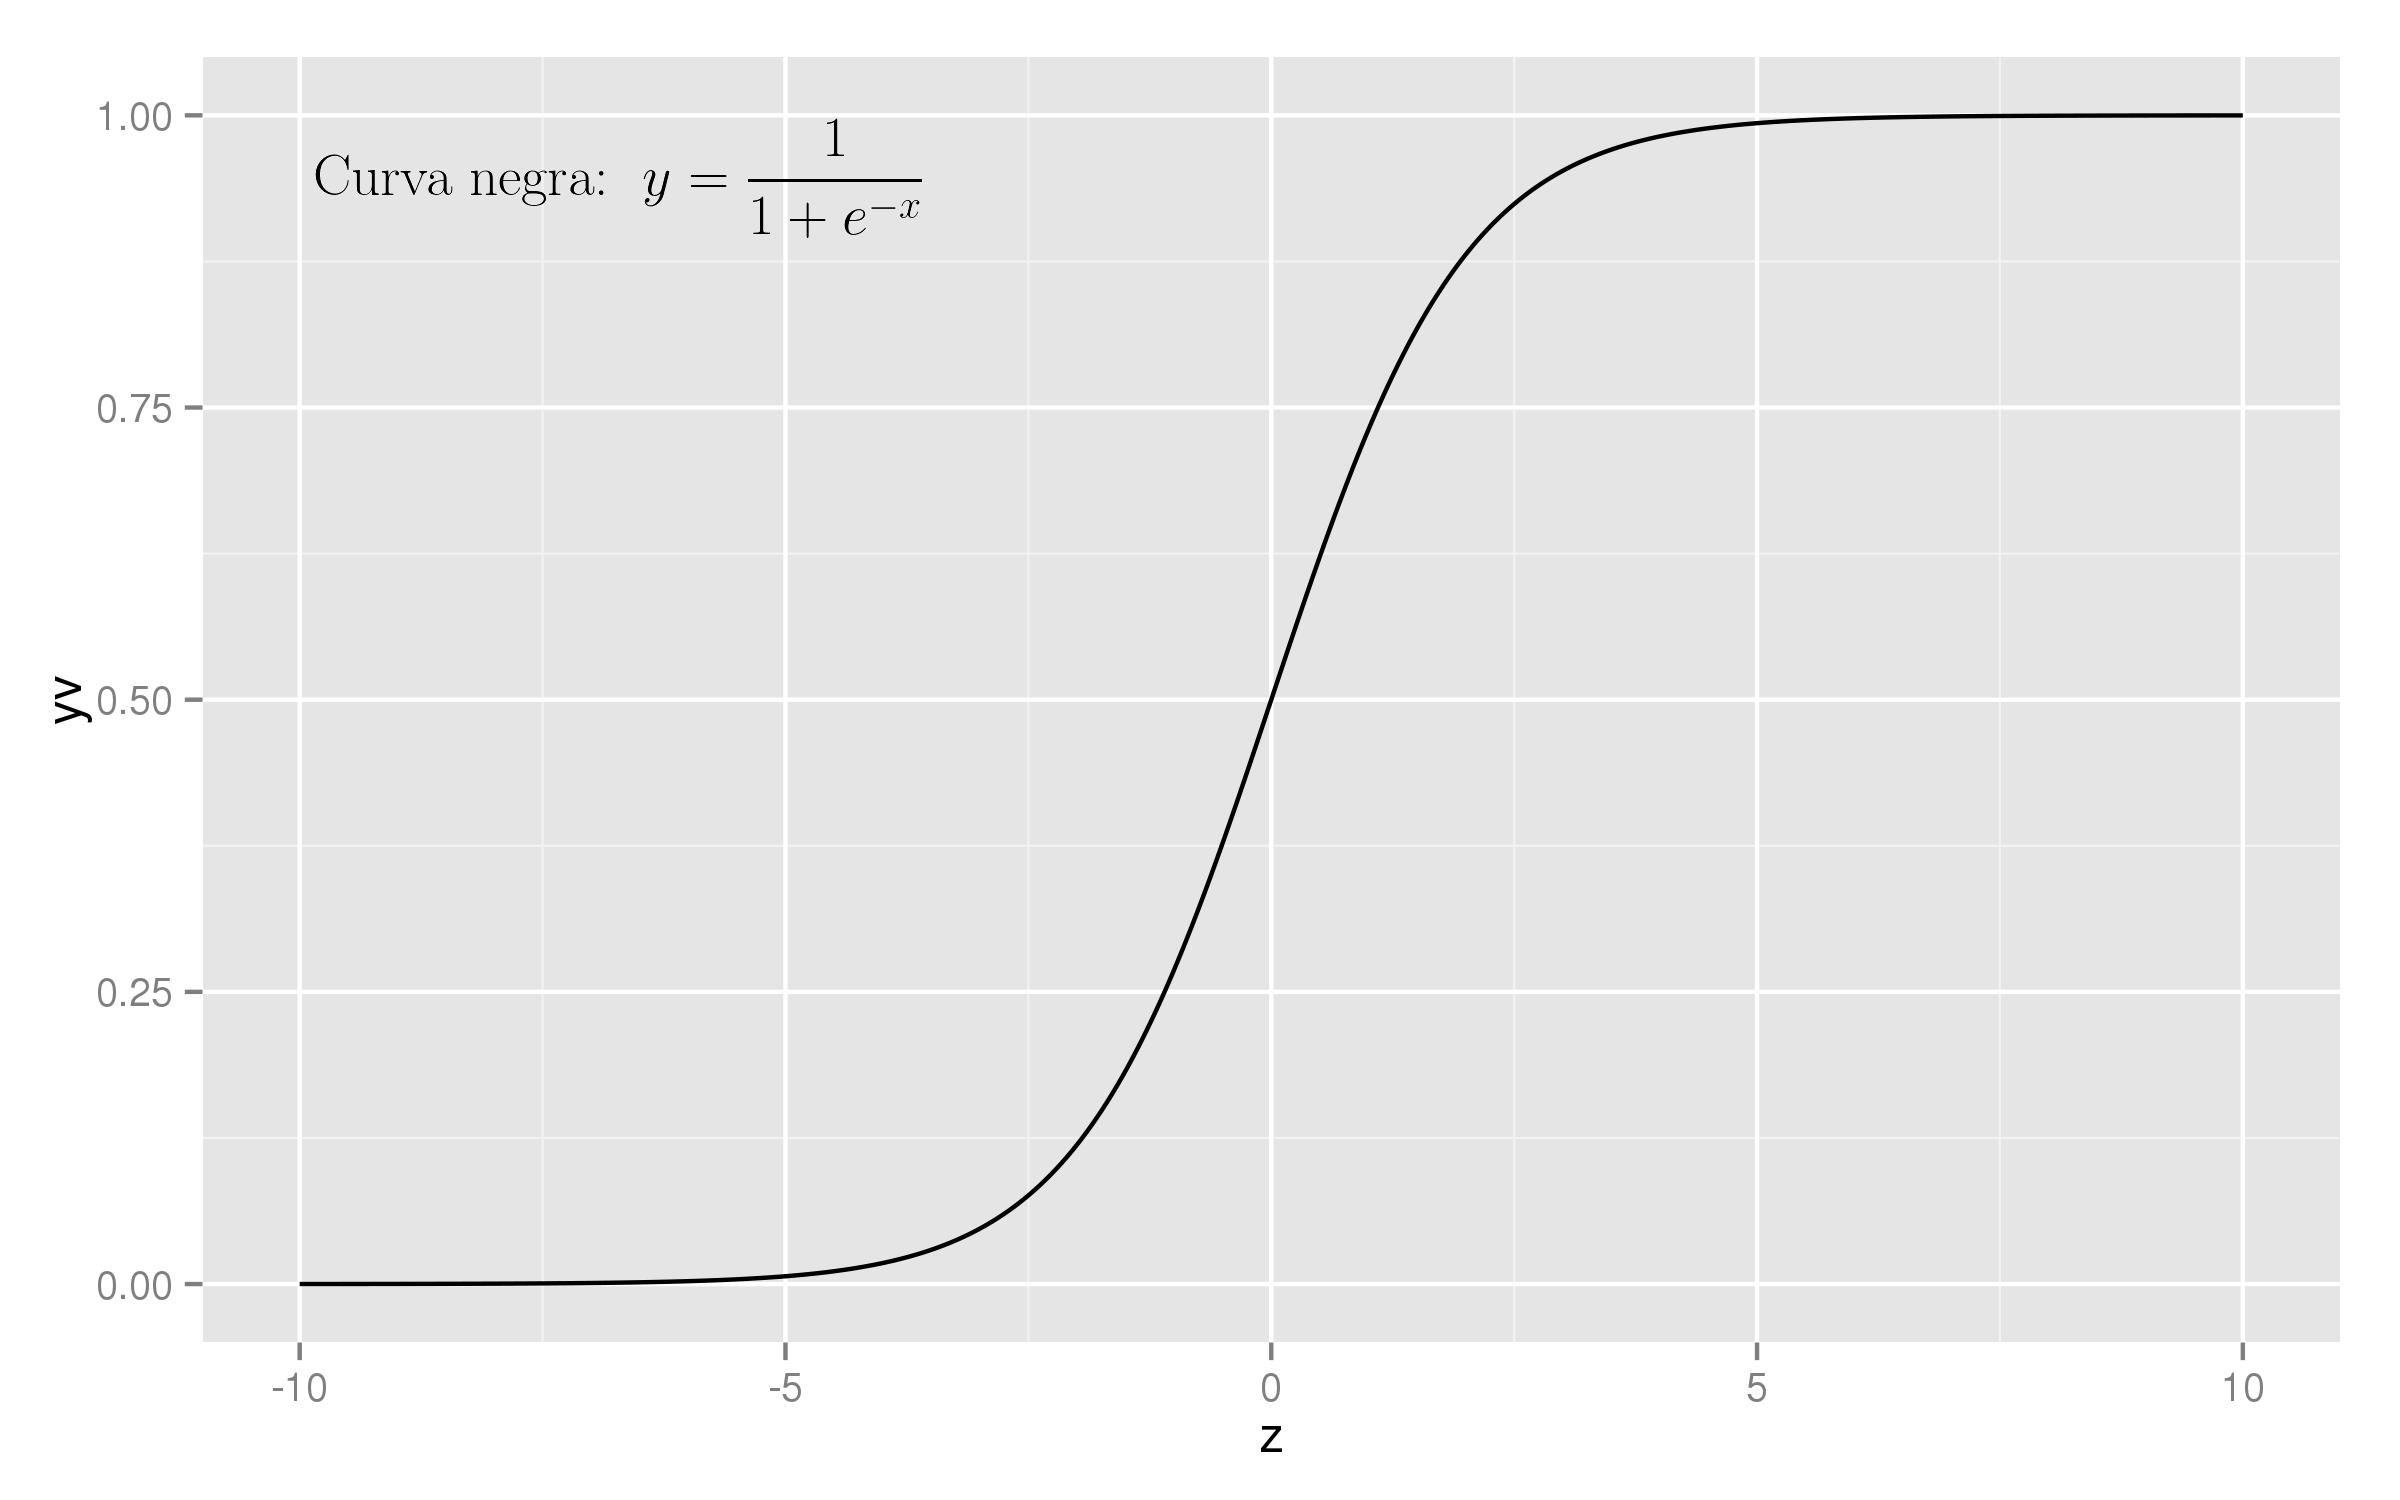
\includegraphics[height=6.8cm]{sigmoidbare.png}
\end{center}
  \end{frame}
 \begin{frame}\frametitle{En el caso de una característica, efecto de variar $\theta$}
\begin{center}
  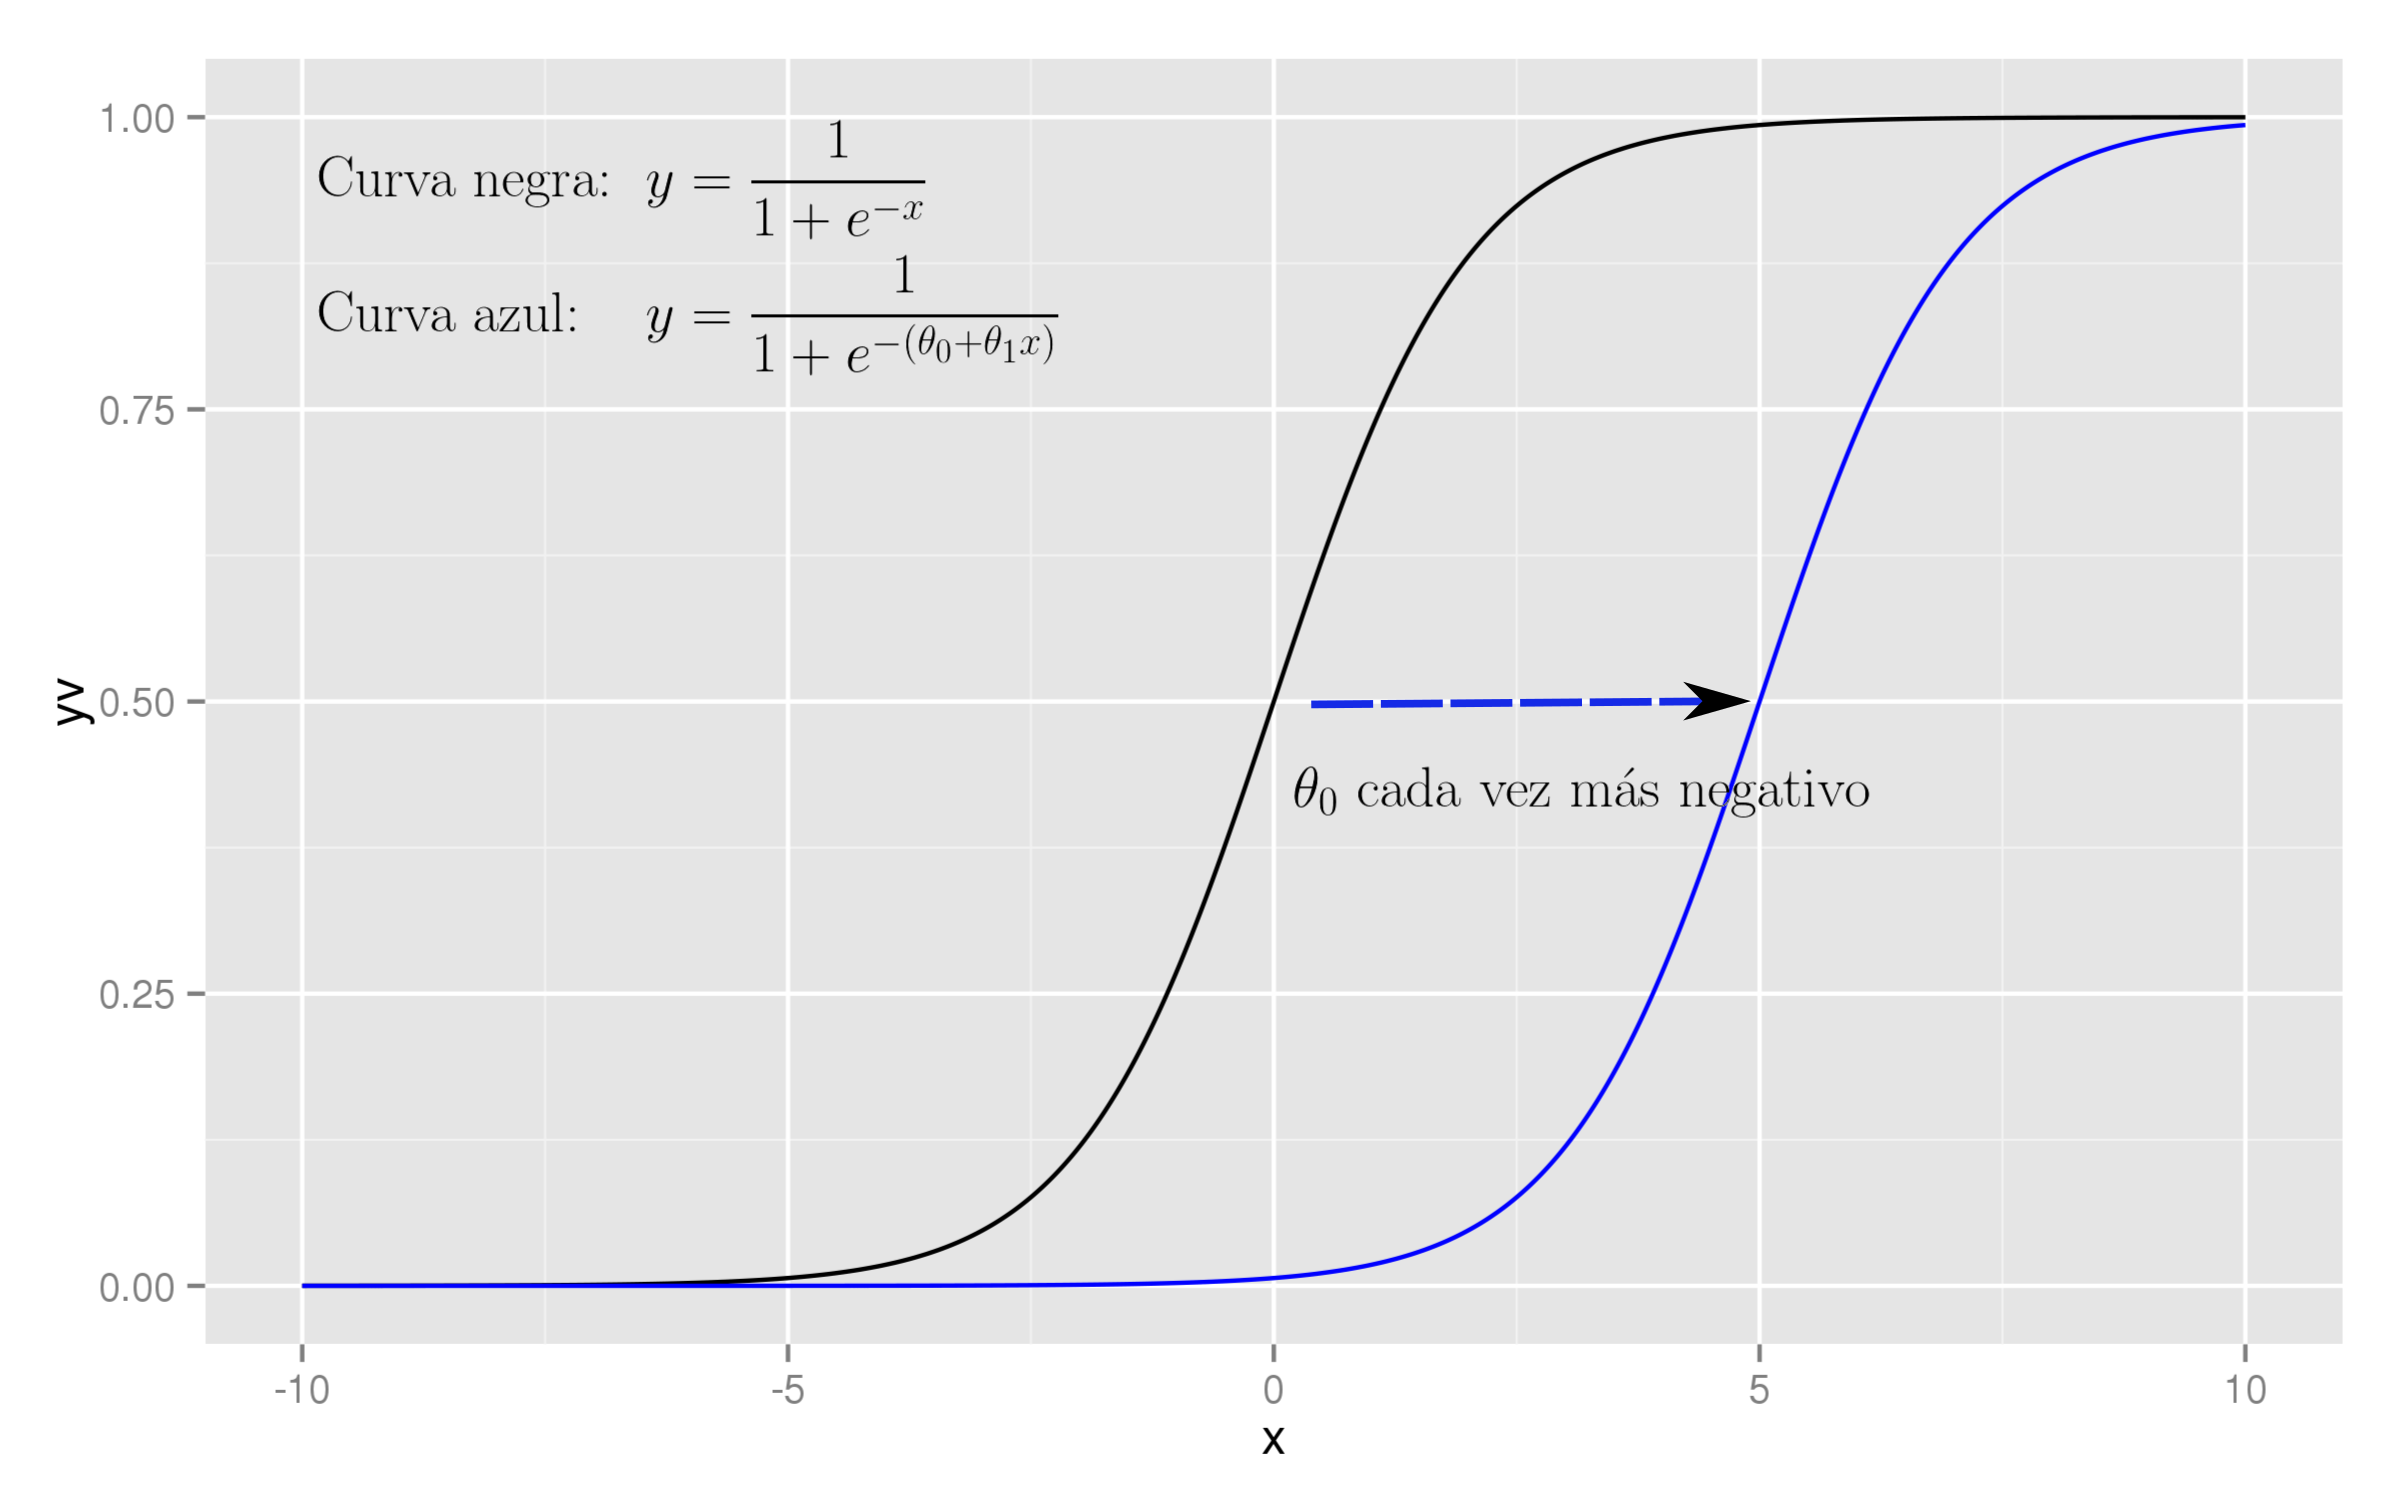
\includegraphics[height=6.8cm]{sigmoidtheta1-ink.png}
\end{center}
 \end{frame}

  \begin{frame}\frametitle{En el caso de una característica, efecto de variar $\theta$}
\begin{center}
  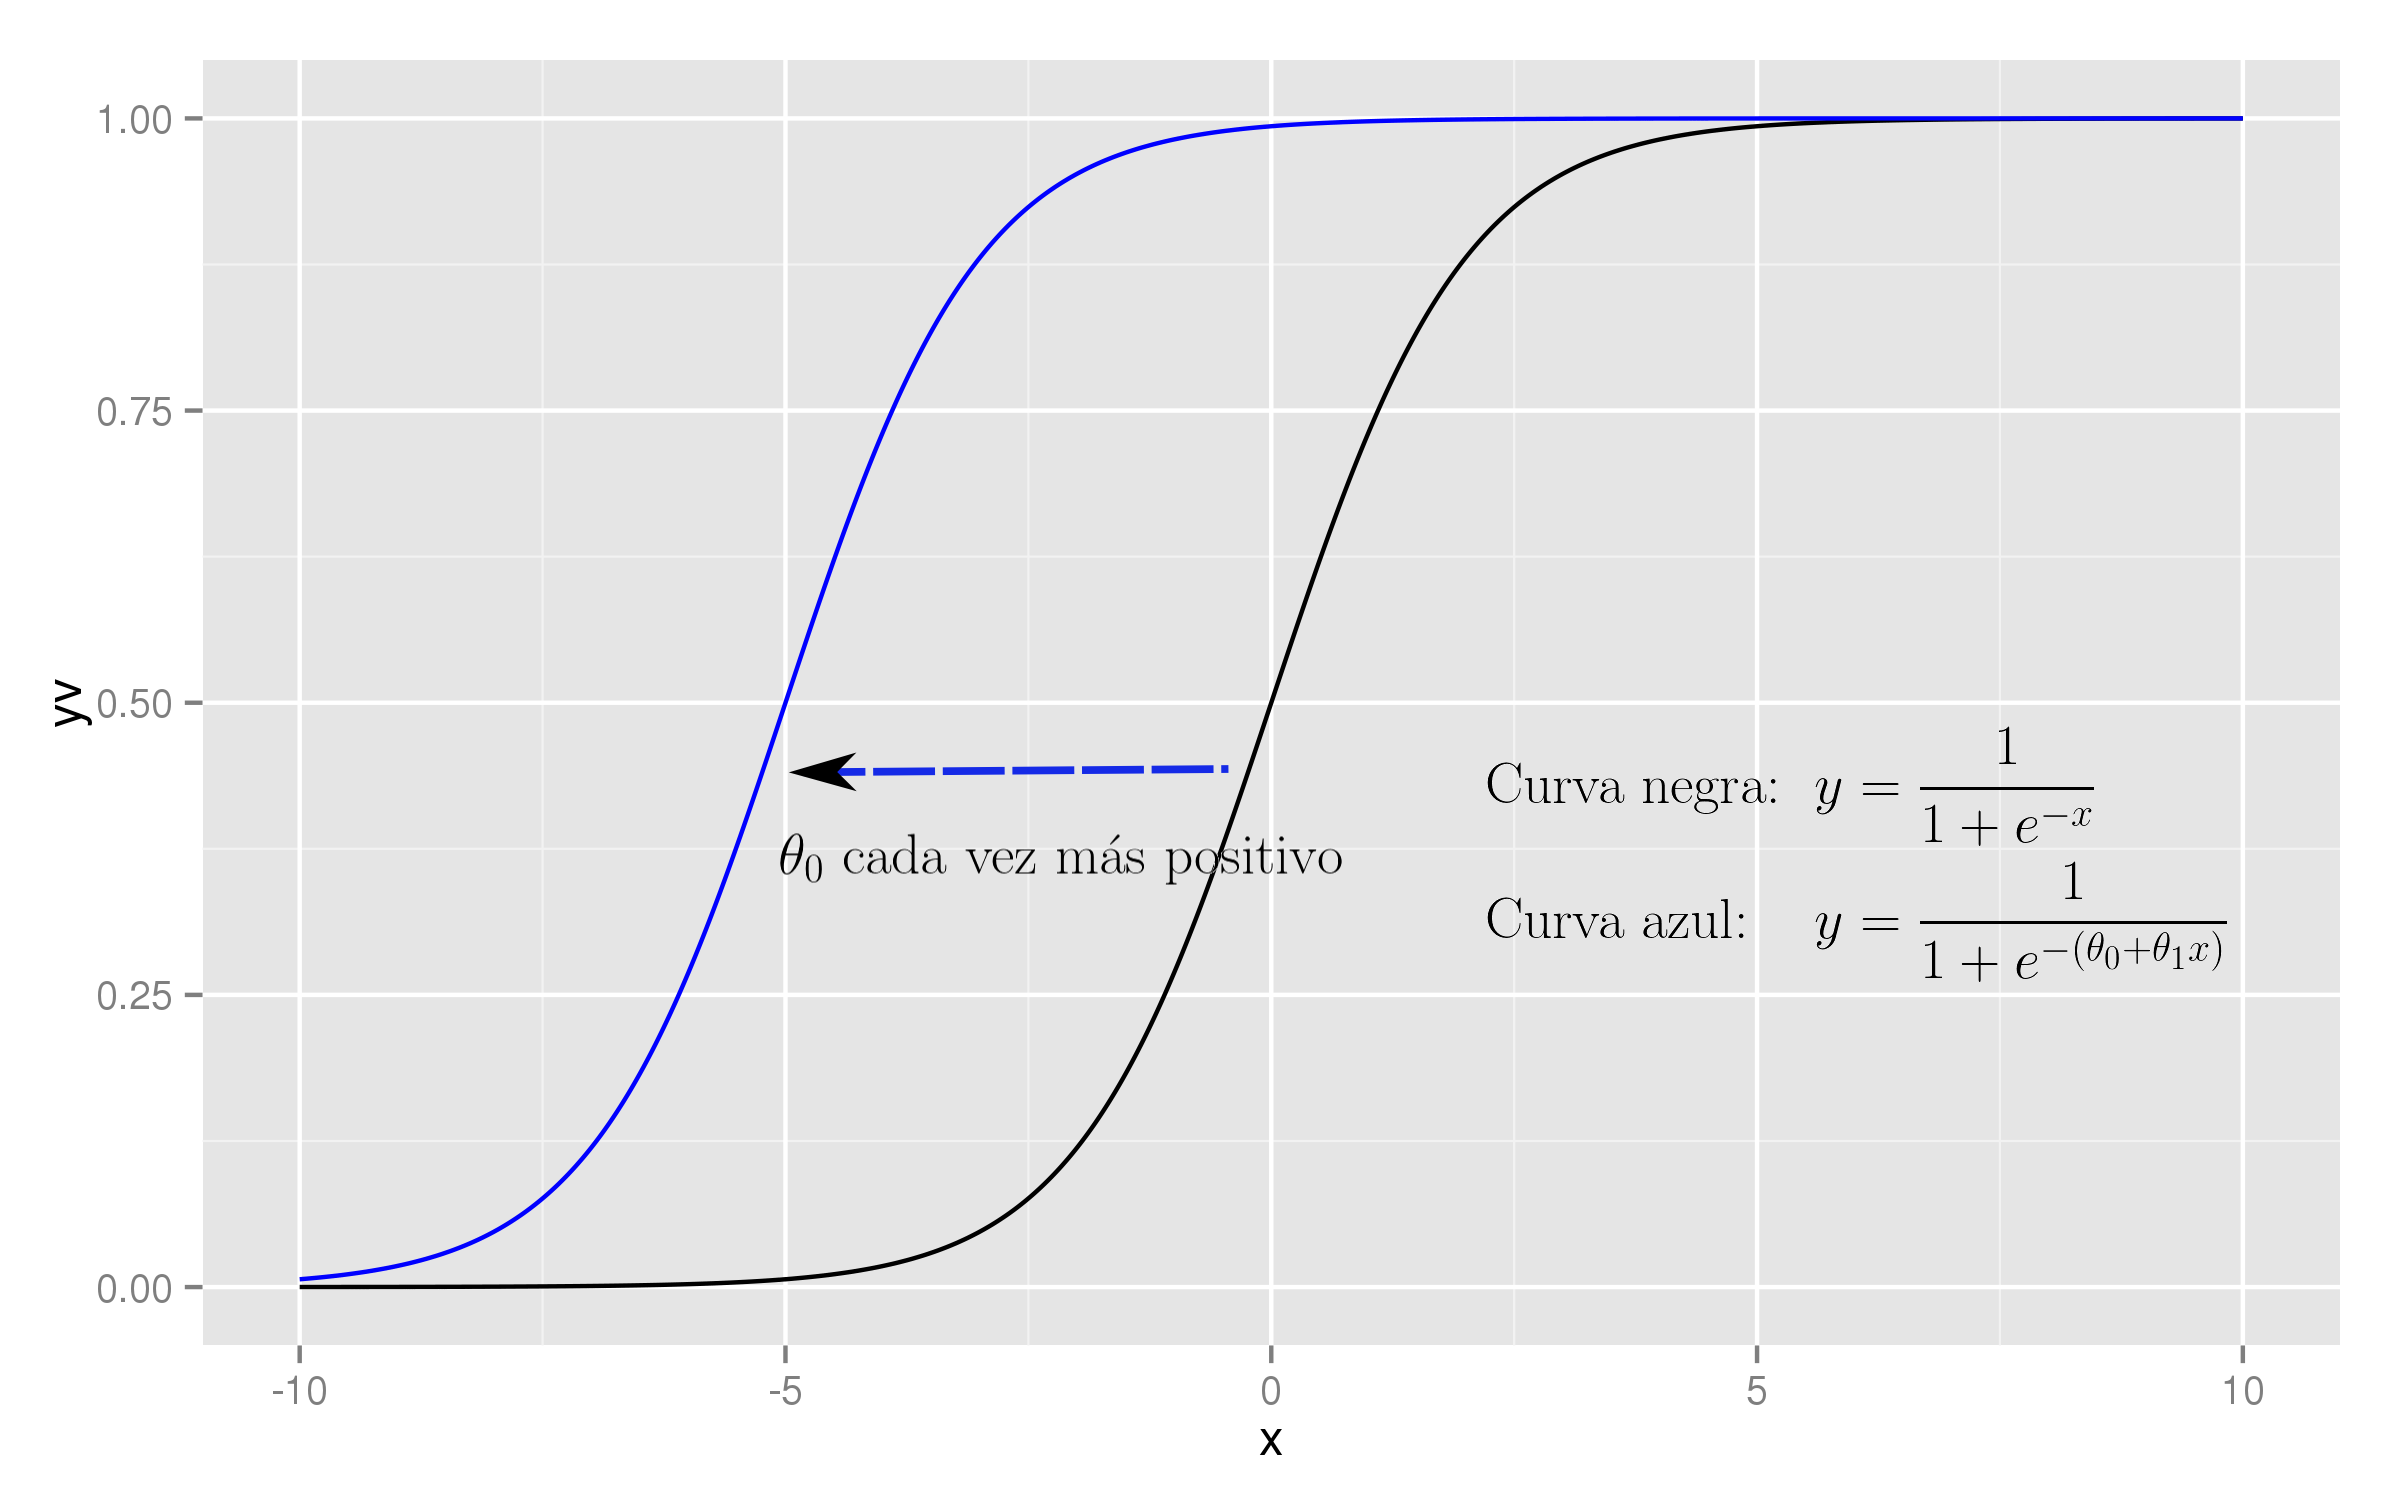
\includegraphics[height=6.8cm]{sigmoidtheta2-ink.png}
\end{center}
 \end{frame}
 \begin{frame}\frametitle{En el caso de una característica, efecto de variar $\theta$}
\begin{center}
  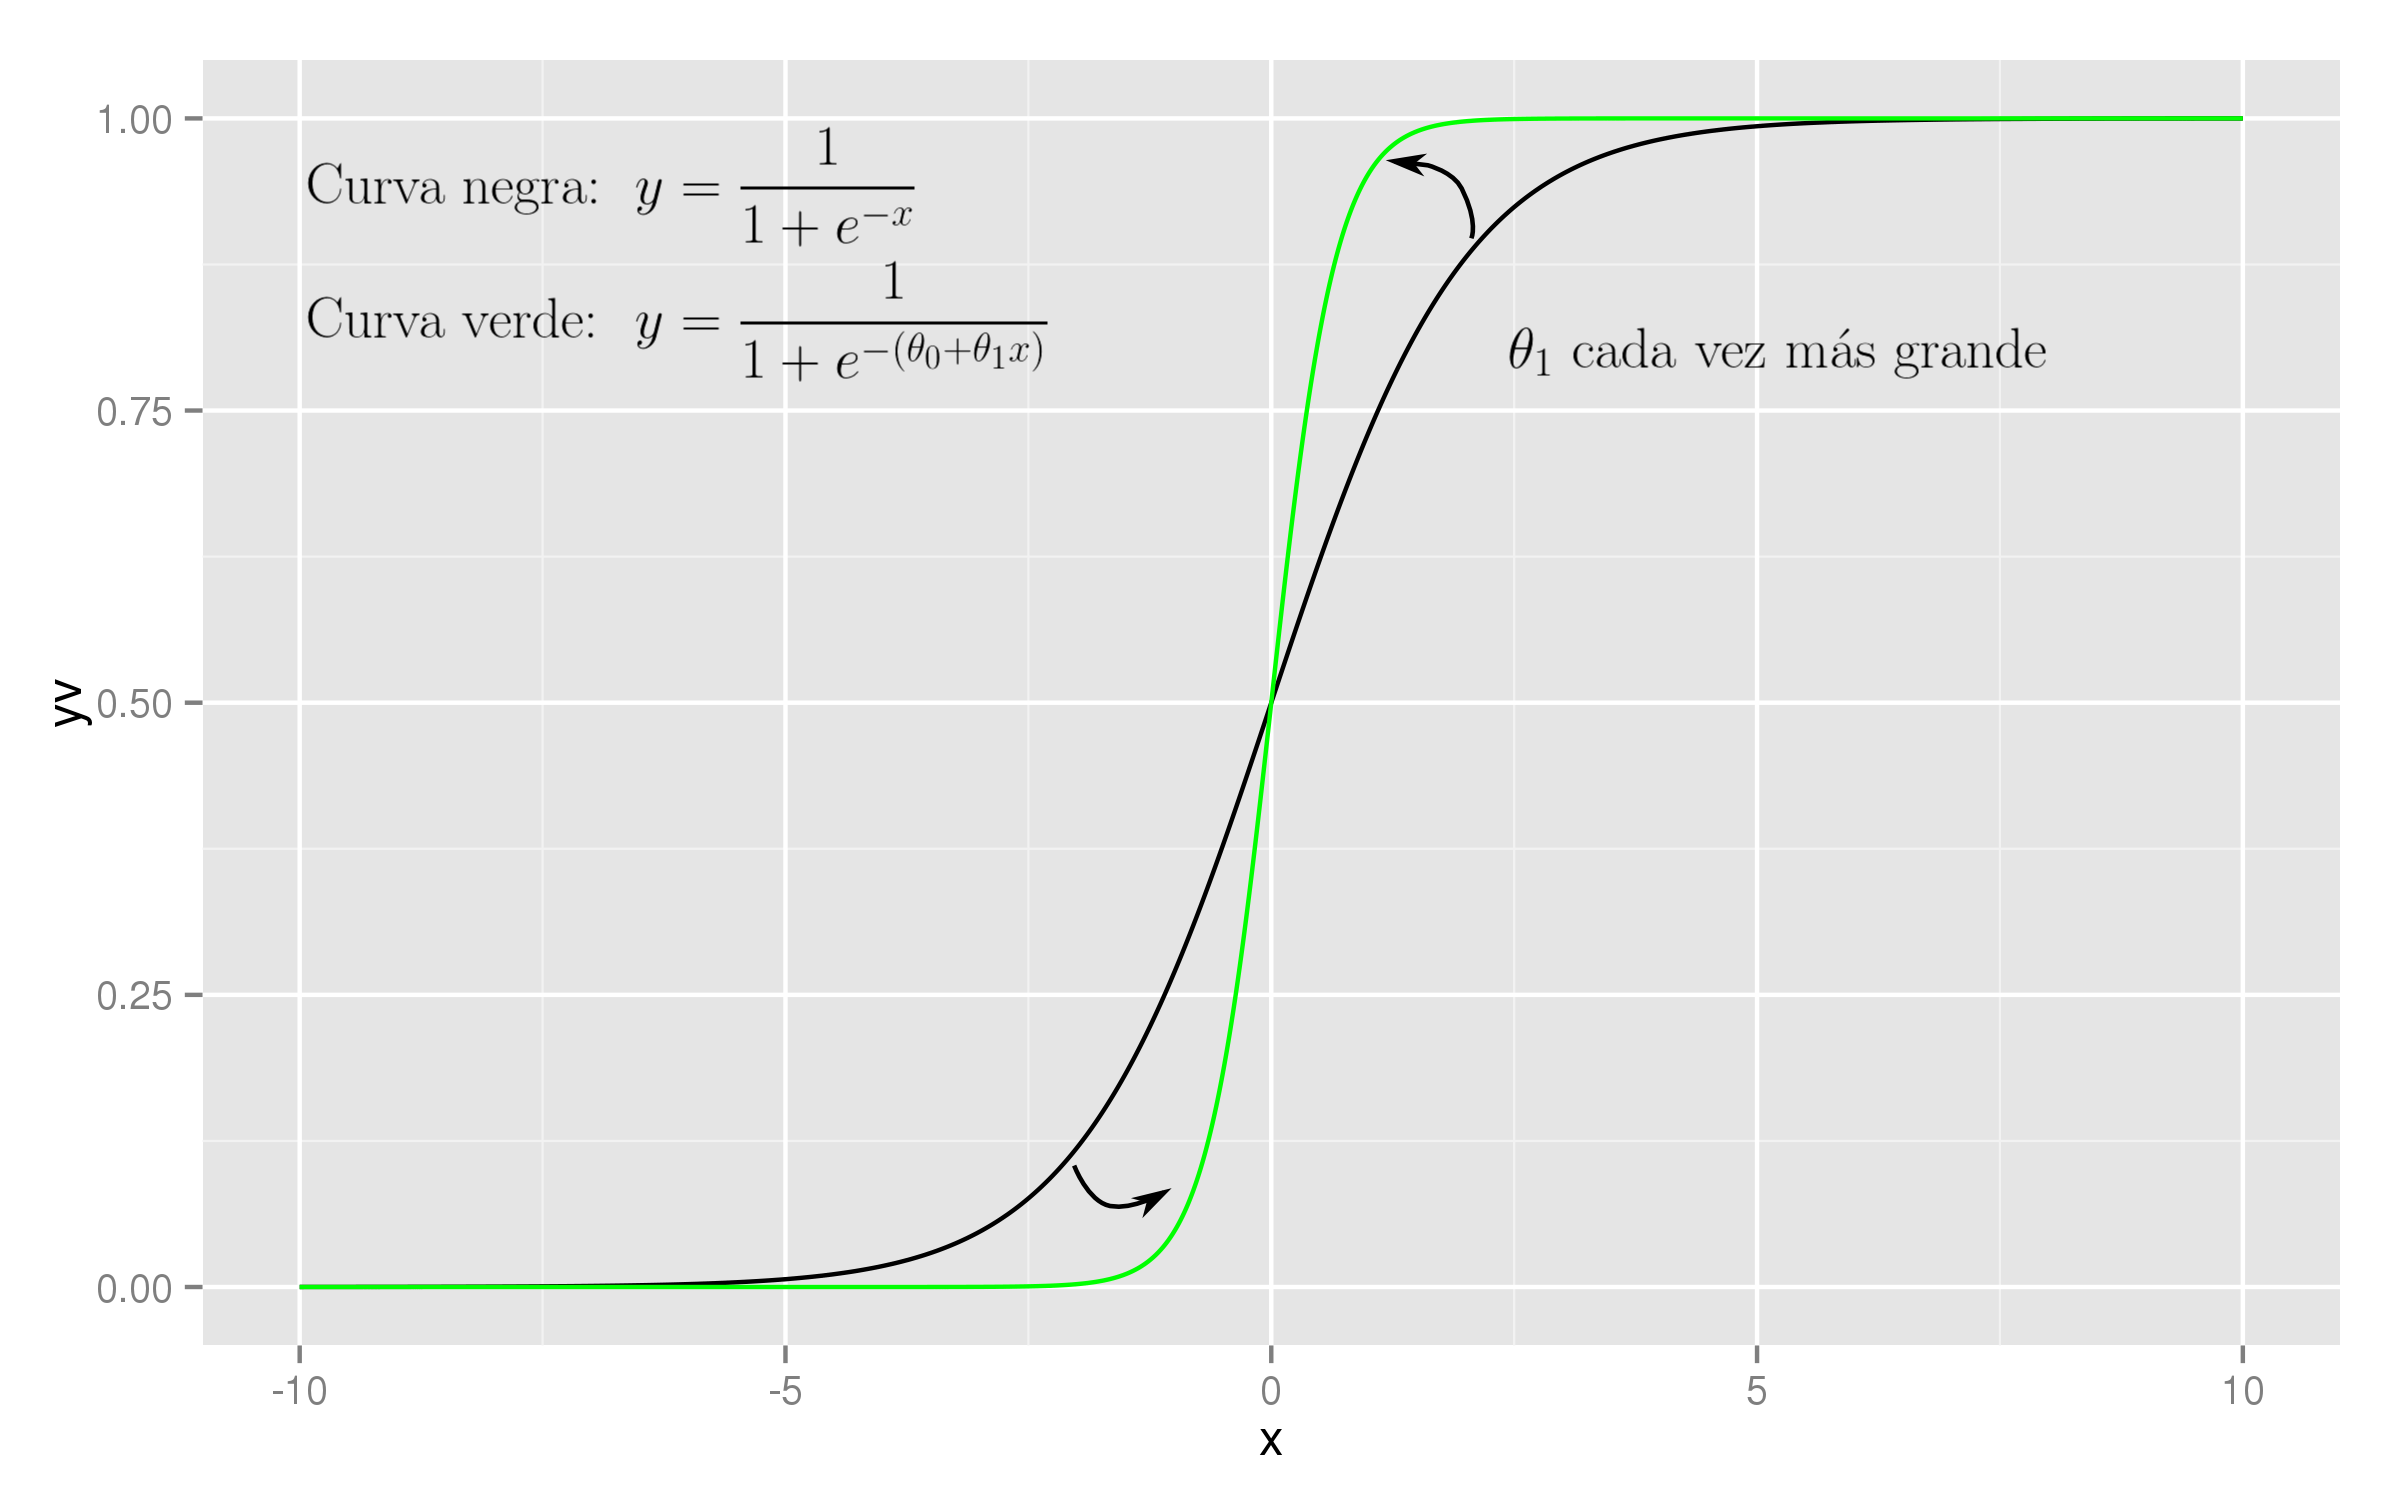
\includegraphics[height=6.8cm]{sigmoidtheta3-ink.png}
\end{center}
 \end{frame}
 \begin{frame}\frametitle{En el caso de una característica, efecto de variar $\theta$}
\begin{center}
  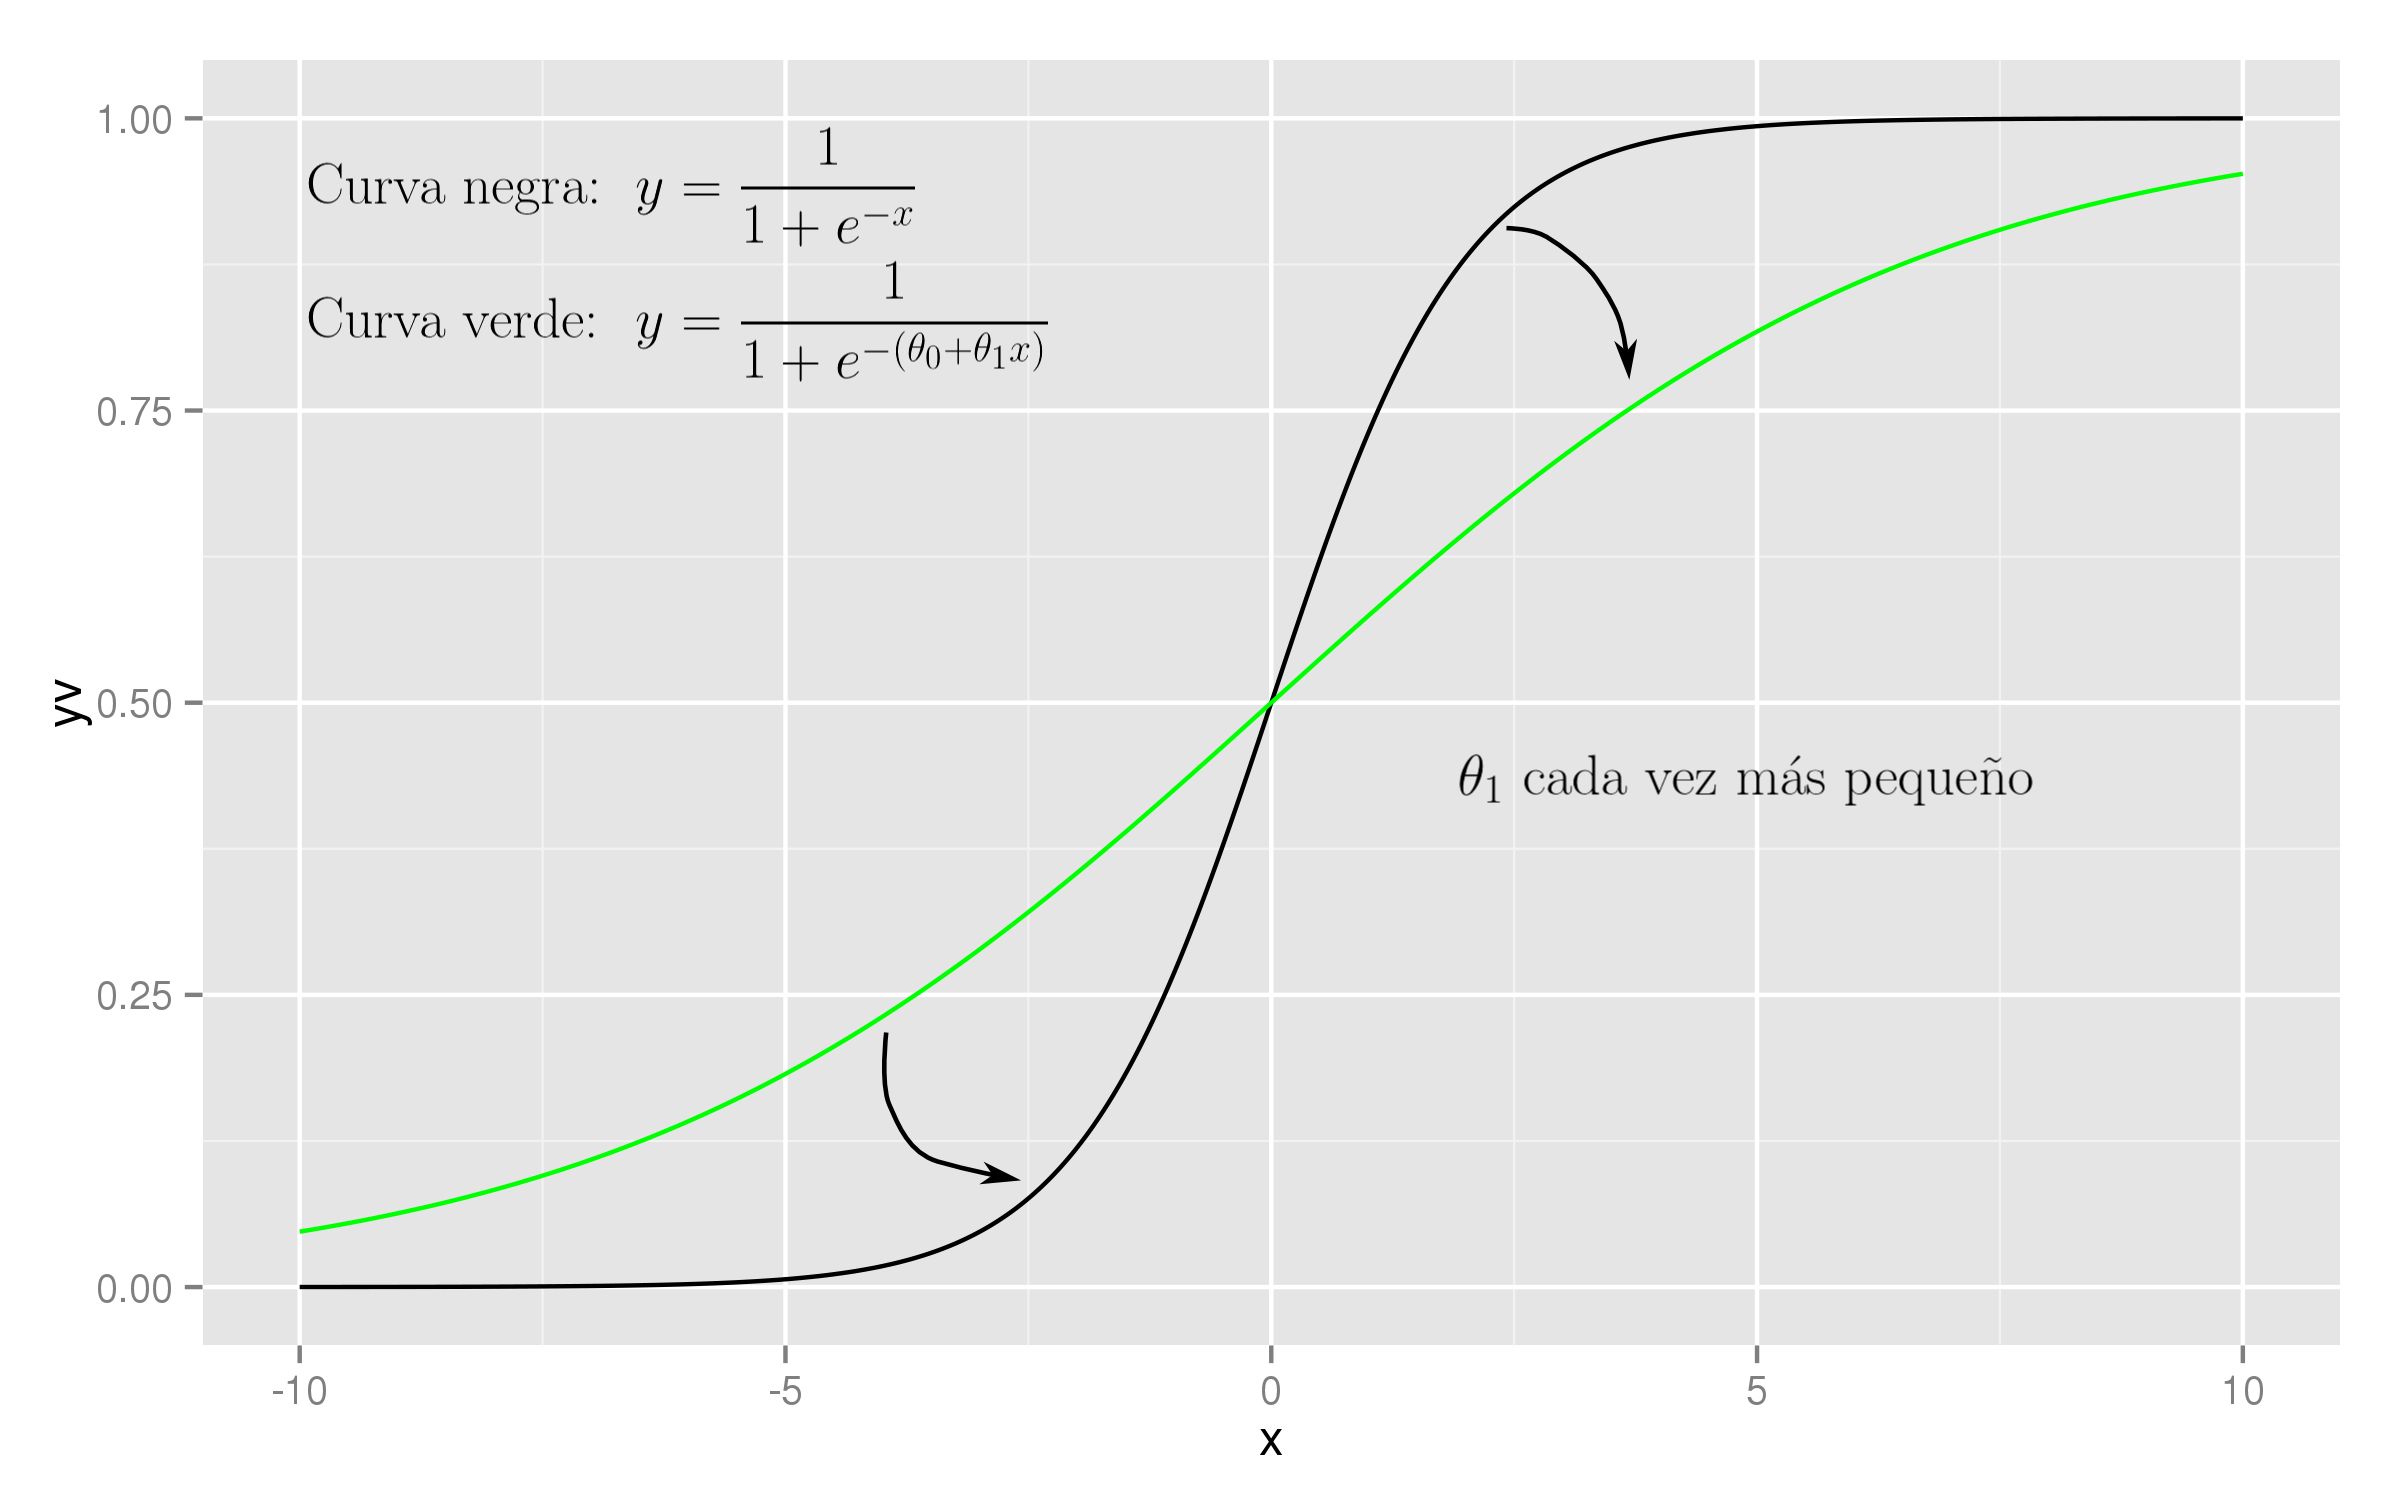
\includegraphics[height=6.8cm]{sigmoidtheta4-ink.png}
\end{center}
 \end{frame}
 \section{Interpretación}
 \begin{frame}\frametitle{Interpretación de $h_\theta(x)$.}
   \begin{block}{Interpretación}
     El valor de $h_\theta(x)$ es la probabilidad de que $y$ tome el valor 1, para ese vector de características $x$, si los parámetros del ajuste son $\theta$.\\
     Es $$h_\theta(x)=\P(y=1|x;\theta),$$
     es decir la probabilidad de que $y=1$ condicionado a $x$ y $\theta$. 
   \end{block}
   \onslide<2->
   Si, dado una nota media PAU, encontramos $h_\theta(x)=0.7$, le diremos al alumno que tiene 70\% de probabilidad de acabar egresando... 
 \end{frame}
 \section{Fronteras de decisión}
 \begin{frame}\frametitle{Regla de decisión, fronteras}
   \begin{itemize}
   \item    Una vez entrenada nuestra regresión logística, tendremos el modelo ajustado $h_{\hat{\theta}}(x)$.
   \item<2->  Recordad que hemos  decidido usar para clasificar la regla de decisión:
     \begin{itemize}
     \item Si $h_\theta(x)\geq 0.5$, clasificamos $\hat{y}$ como 1.
     \item Si $h_\theta(x)<0.5$, clasificamos $\hat{y}$ como 0.
     \end{itemize}
   \item<3-> Pero $h_\theta(x)=g(x^T\theta)$, por lo que 
     \begin{itemize}
     \item $h_\theta(x)\geq 0.5\Leftrightarrow x^T\theta\geq 0$ y
     \item $h_\theta(x)< 0.5\Leftrightarrow x^T\theta<0$. 
     \end{itemize}
   \item<4-> Así que, en realidad, hemos especificado así una región de decisión cuya frontera es $$x^T\theta=0.$$
   \end{itemize}
   
 \end{frame}
 \begin{frame}\frametitle{Región de decisión ilustrada con dos características}
%% \begin{tabularx}{m{.60\textwidth}@{\extracolsep{1mm}} m{.40\textwidth}}
%%      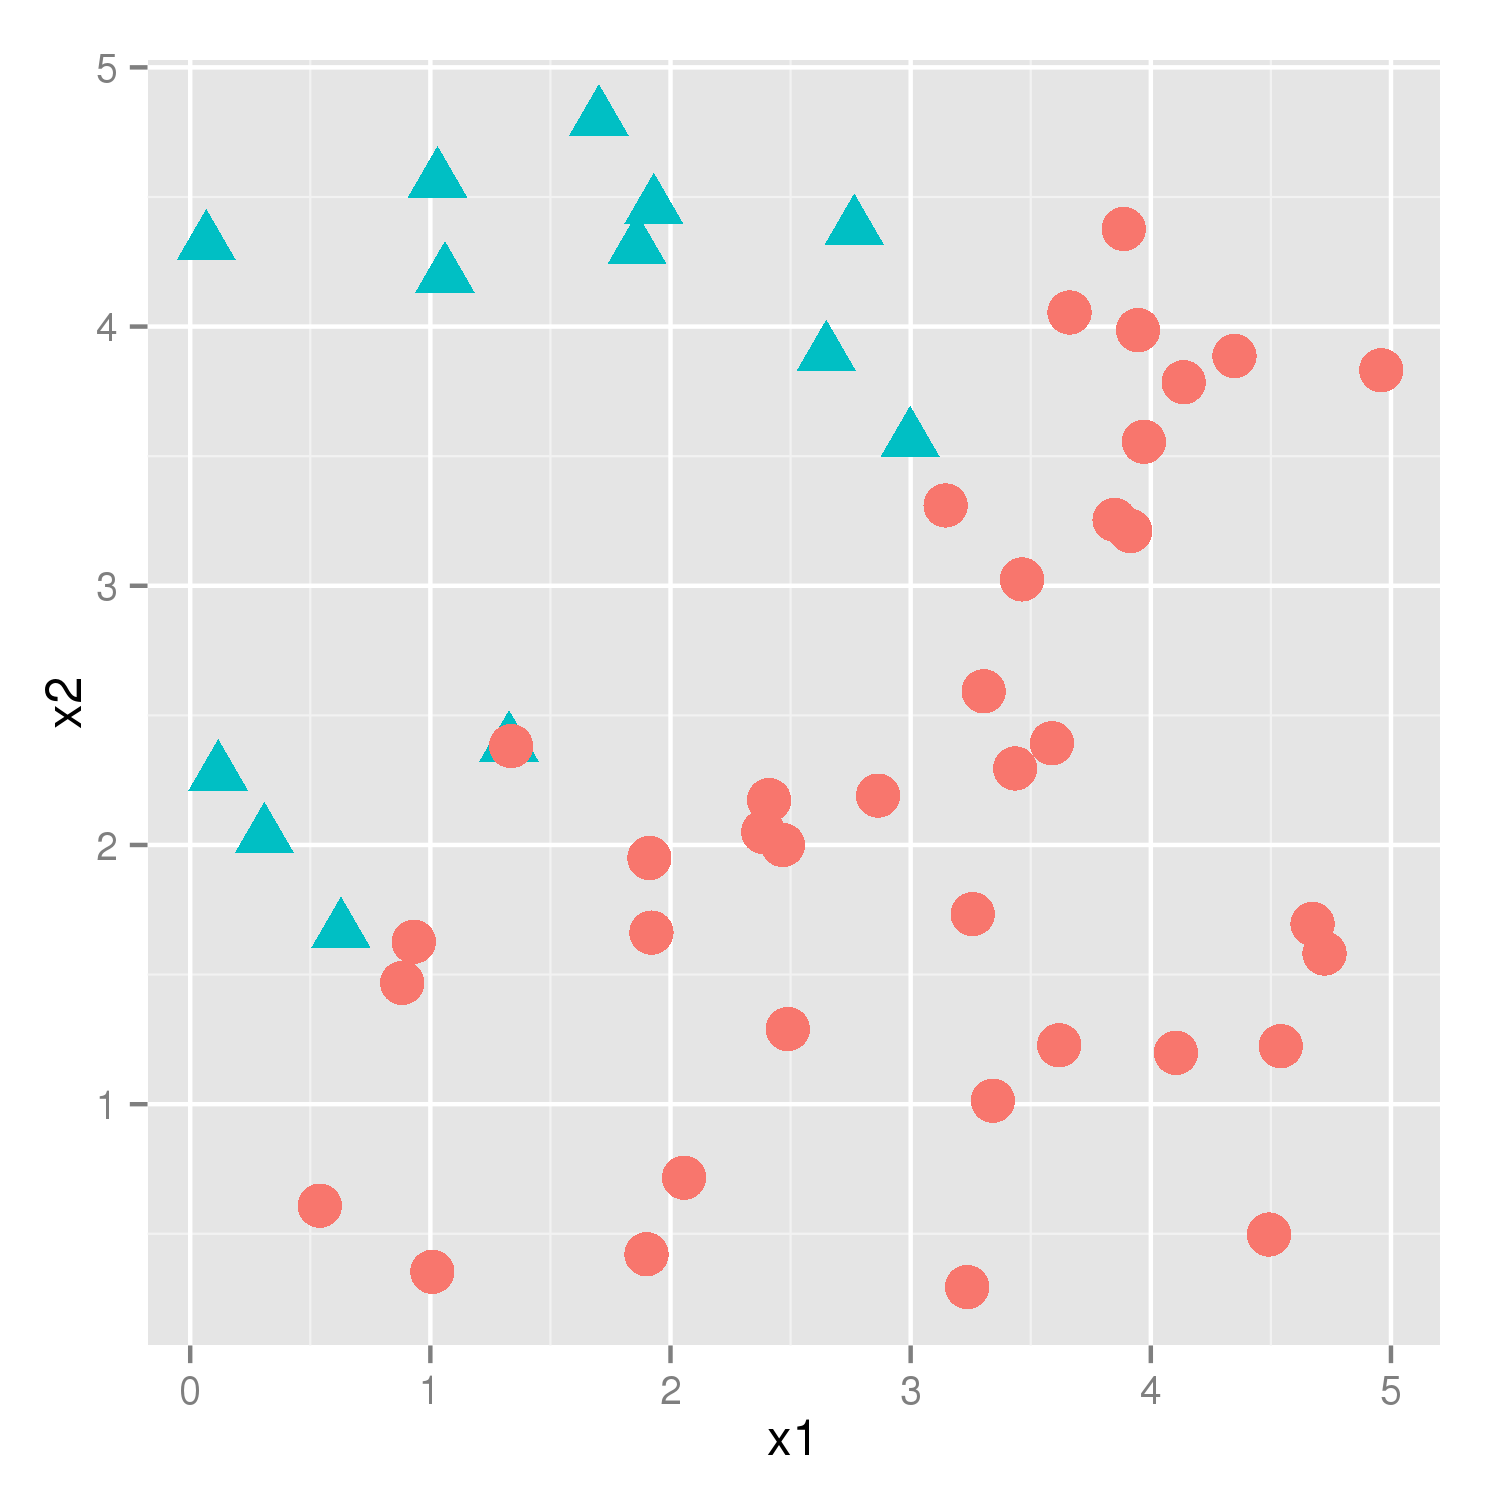
\includegraphics[height=5cm,width=5cm]{decisionboundaries1.png}& 
%%      \begin{minipage}{6.8cm}
%%      Dos características, $x1$ y $x2$, azul representa un valor 1 para $y$, (rojo un valor 0).  \\
%%      \end{minipage}
%%    \end{tabularx}
%%  \begin{tabularx}{\textwidth}{ Xp{5cm}}
%%   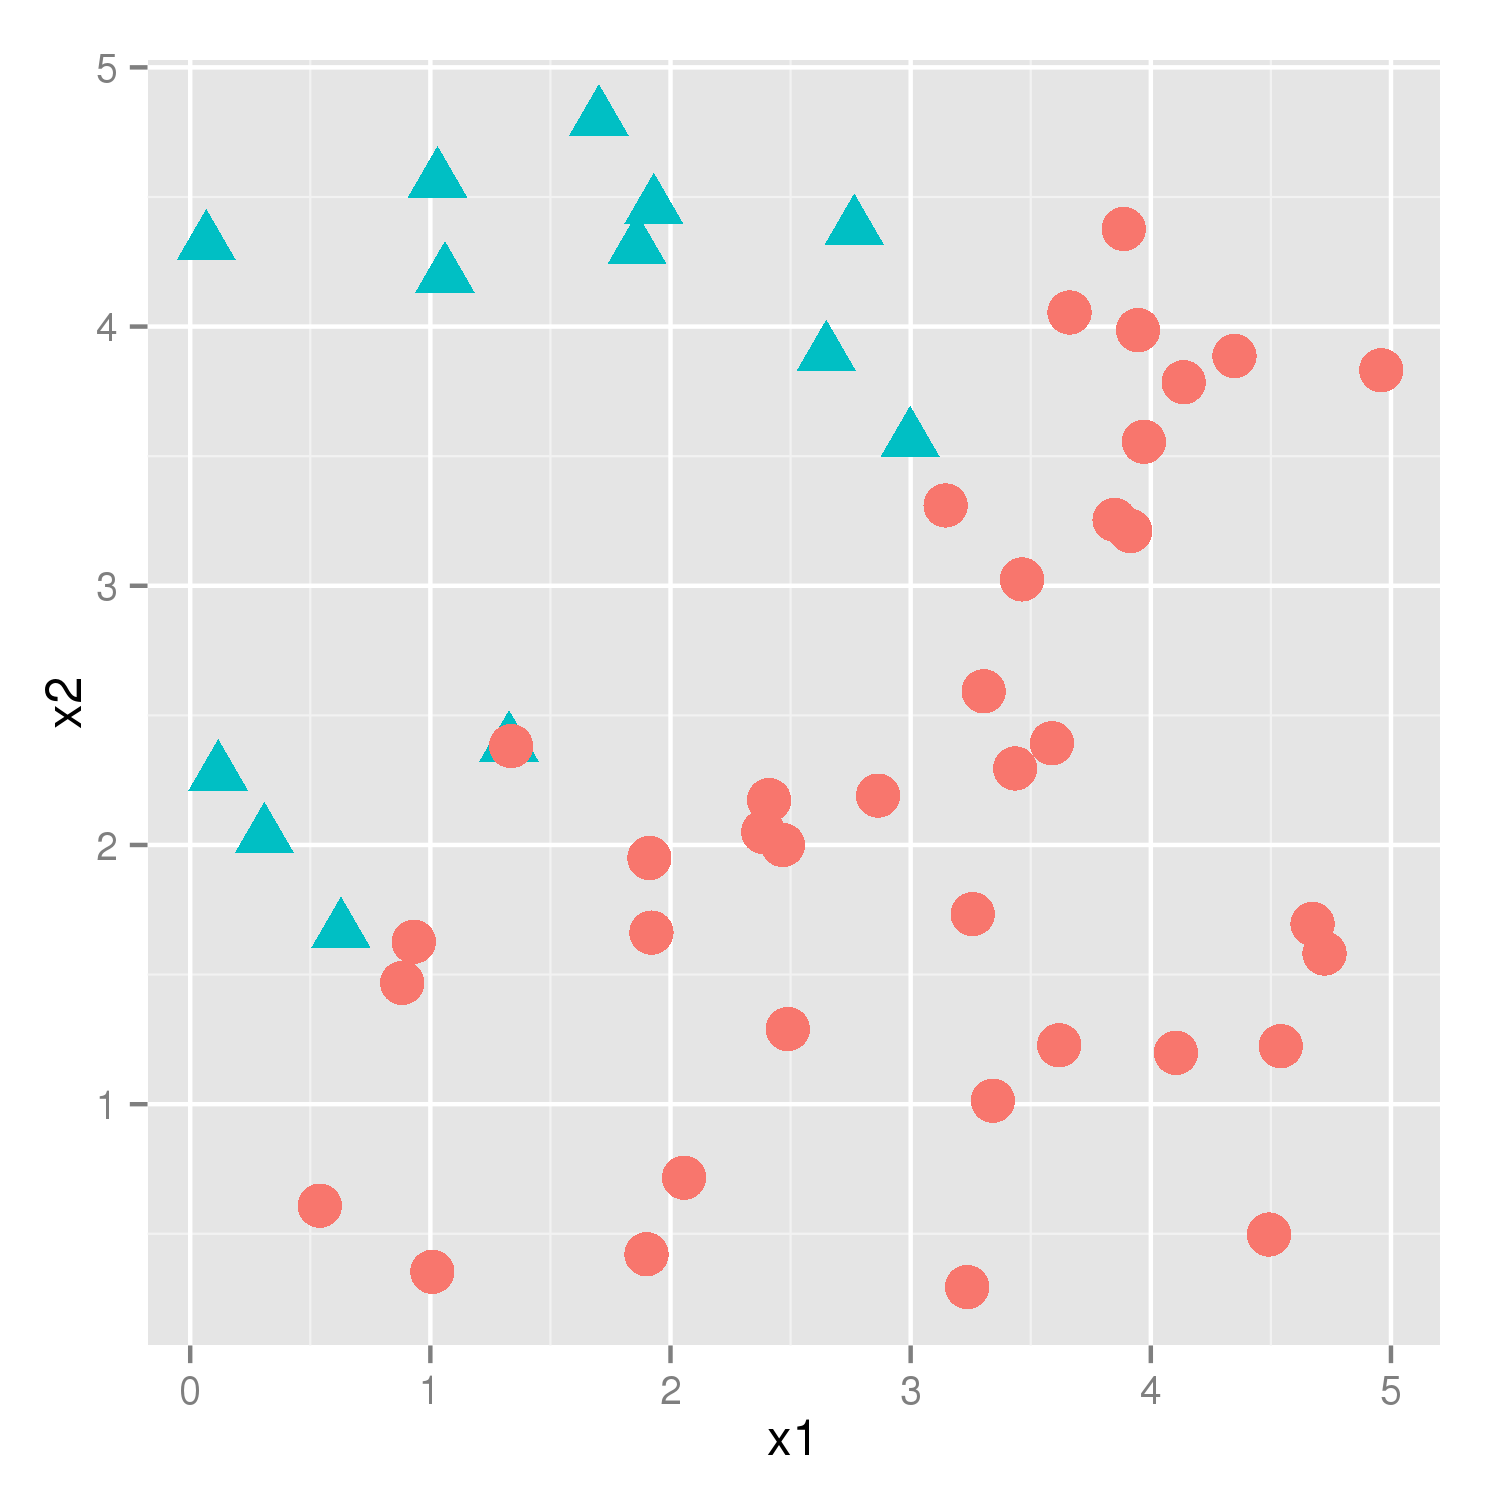
\includegraphics[height=5cm,width=5cm]{decisionboundaries1.png} &
%%        \begin{minipage}[t][5cm][t]{4.5cm}
%%          \footnotesize
%%      Dos características, $x1$ y $x2$\\
%%      azul $\leftrightarrow y=1$; rojo $\leftrightarrow y=0$
%%      \end{minipage}\\
%% \end{tabularx}
%%    \begin{tabular}{ll}
          \begin{minipage}[t][5cm][t]{5.5cm}
  \raisebox{-\height}{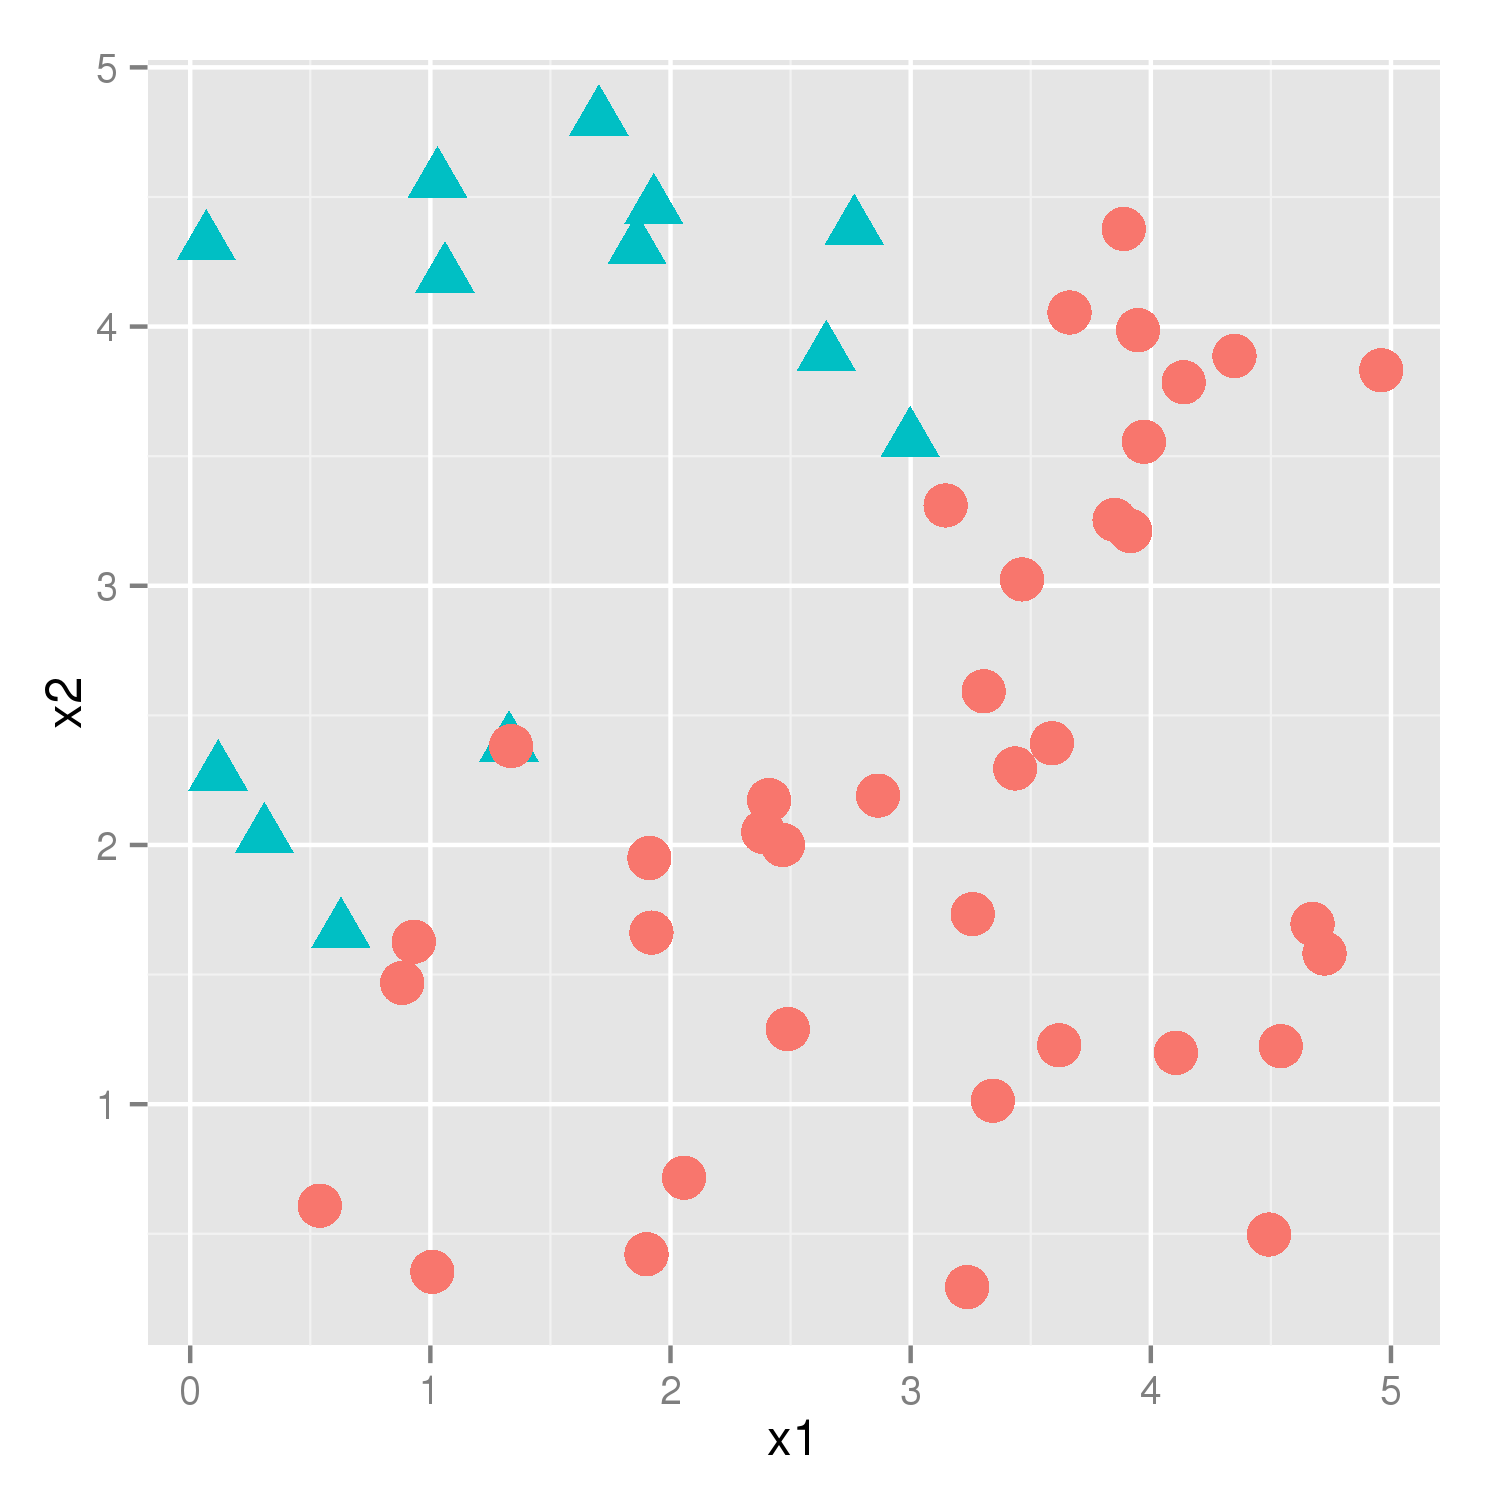
\includegraphics[height=5cm,width=5cm]{decisionboundaries1.png}}
          \end{minipage}
%          &
       \begin{minipage}[t][5cm][t]{4.5cm}
         \footnotesize
     Dos características, $x1$ y $x2$\\
     azul $\leftrightarrow y=1$; rojo $\leftrightarrow y=0$
     \end{minipage}\\
%\end{tabular}

 \end{frame}
 \begin{frame}\frametitle{Región de decisión ilustrada con dos características}
 \begin{minipage}[t][5cm][t]{5.5cm}
  \raisebox{-\height}{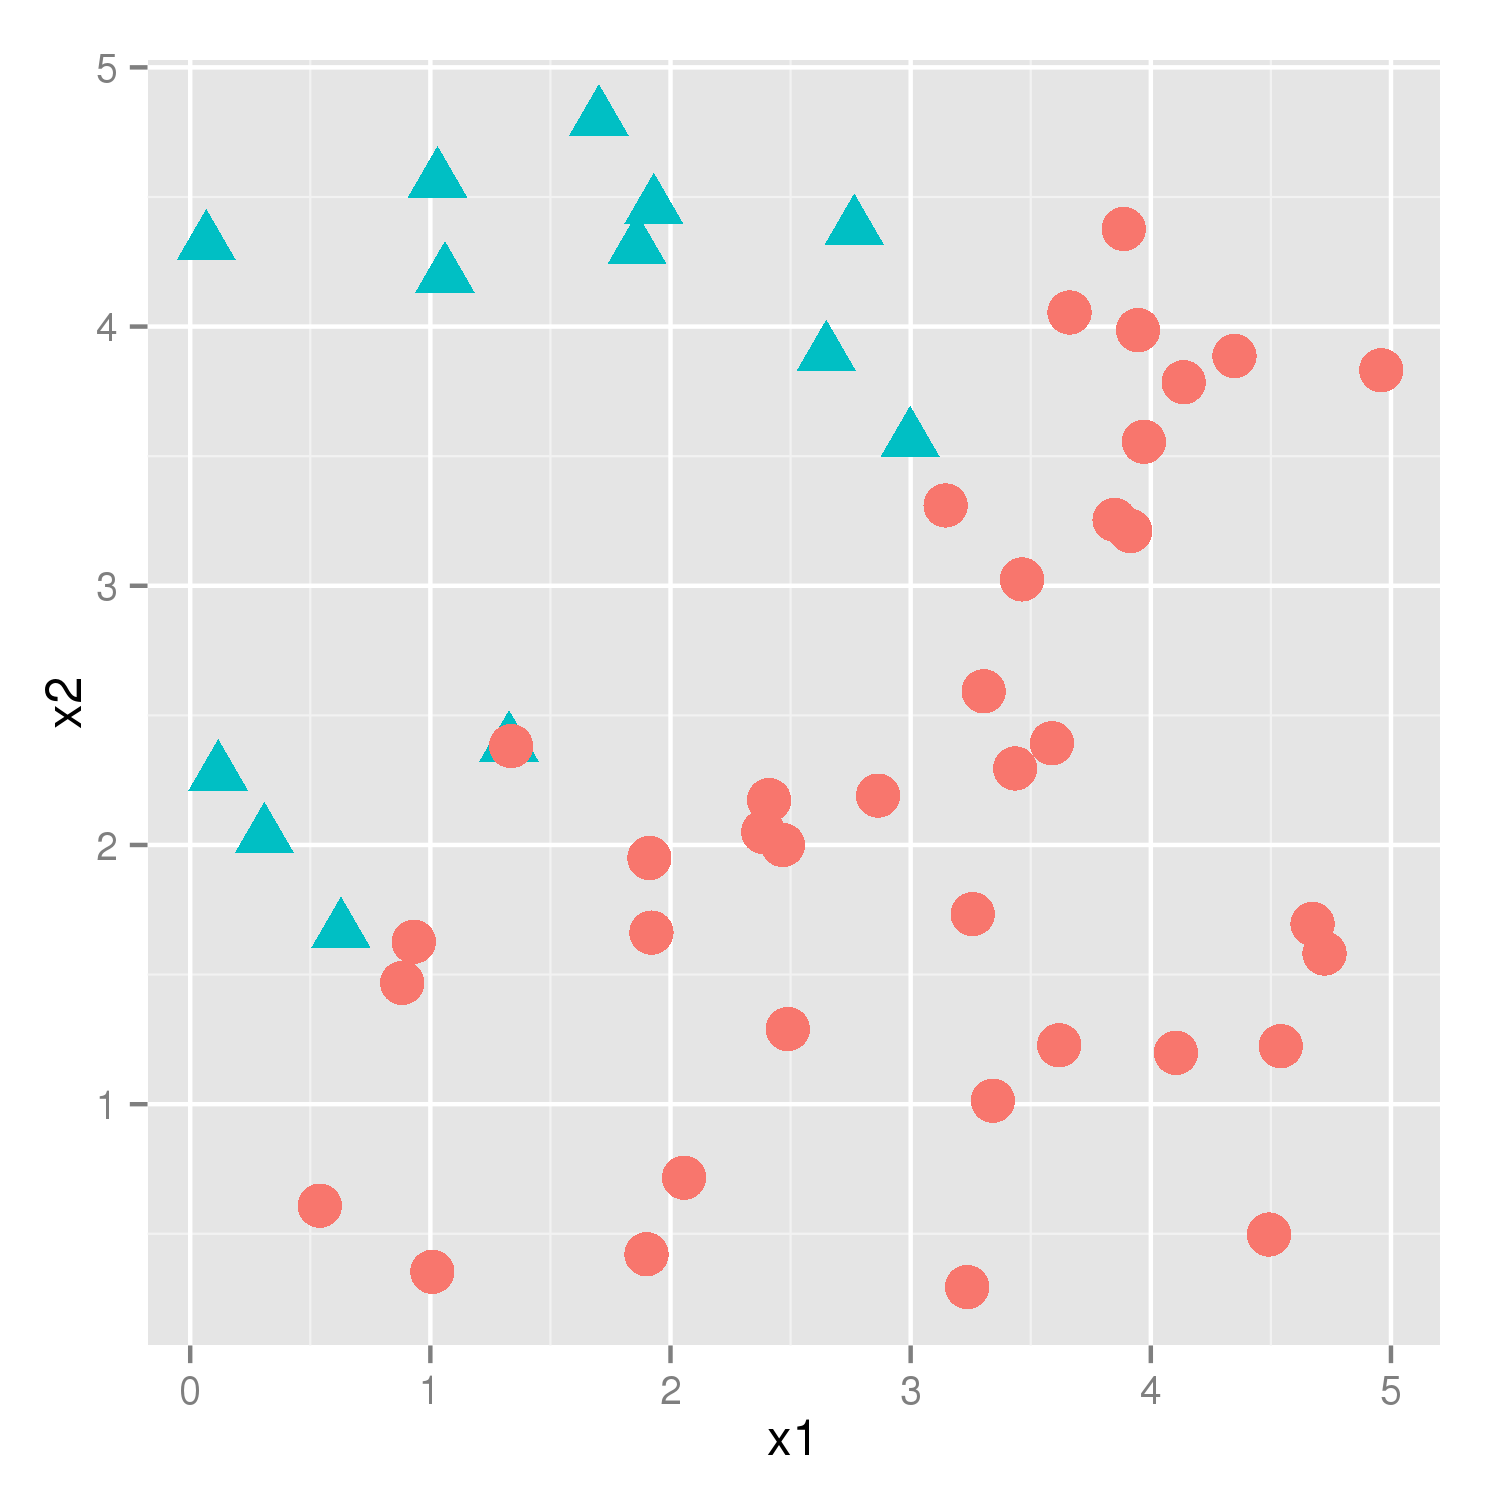
\includegraphics[height=5cm,width=5cm]{decisionboundaries1.png}}
          \end{minipage}
%          &
       \begin{minipage}[t][5cm][t]{4.5cm}
         \footnotesize
     Dos características, $x1$ y $x2$\\
     azul $\leftrightarrow y=1$; rojo $\leftrightarrow y=0$\\
     Tenemos: 
     \begin{itemize}
     \item $\theta=(\theta_0,\theta_1,\theta_2)$,
     \item $x=(1,x_1,x_2)$,
     \end{itemize}
     por lo que la frontera de la región es $$\theta_0+\theta_1x_1+\theta_2x_2=0.$$ 
     \end{minipage}\\
%\end{tabular}

 \end{frame}
  \begin{frame}\frametitle{Región de decisión ilustrada con dos características}
 \begin{minipage}[t][5cm][t]{5.5cm}
  \raisebox{-\height}{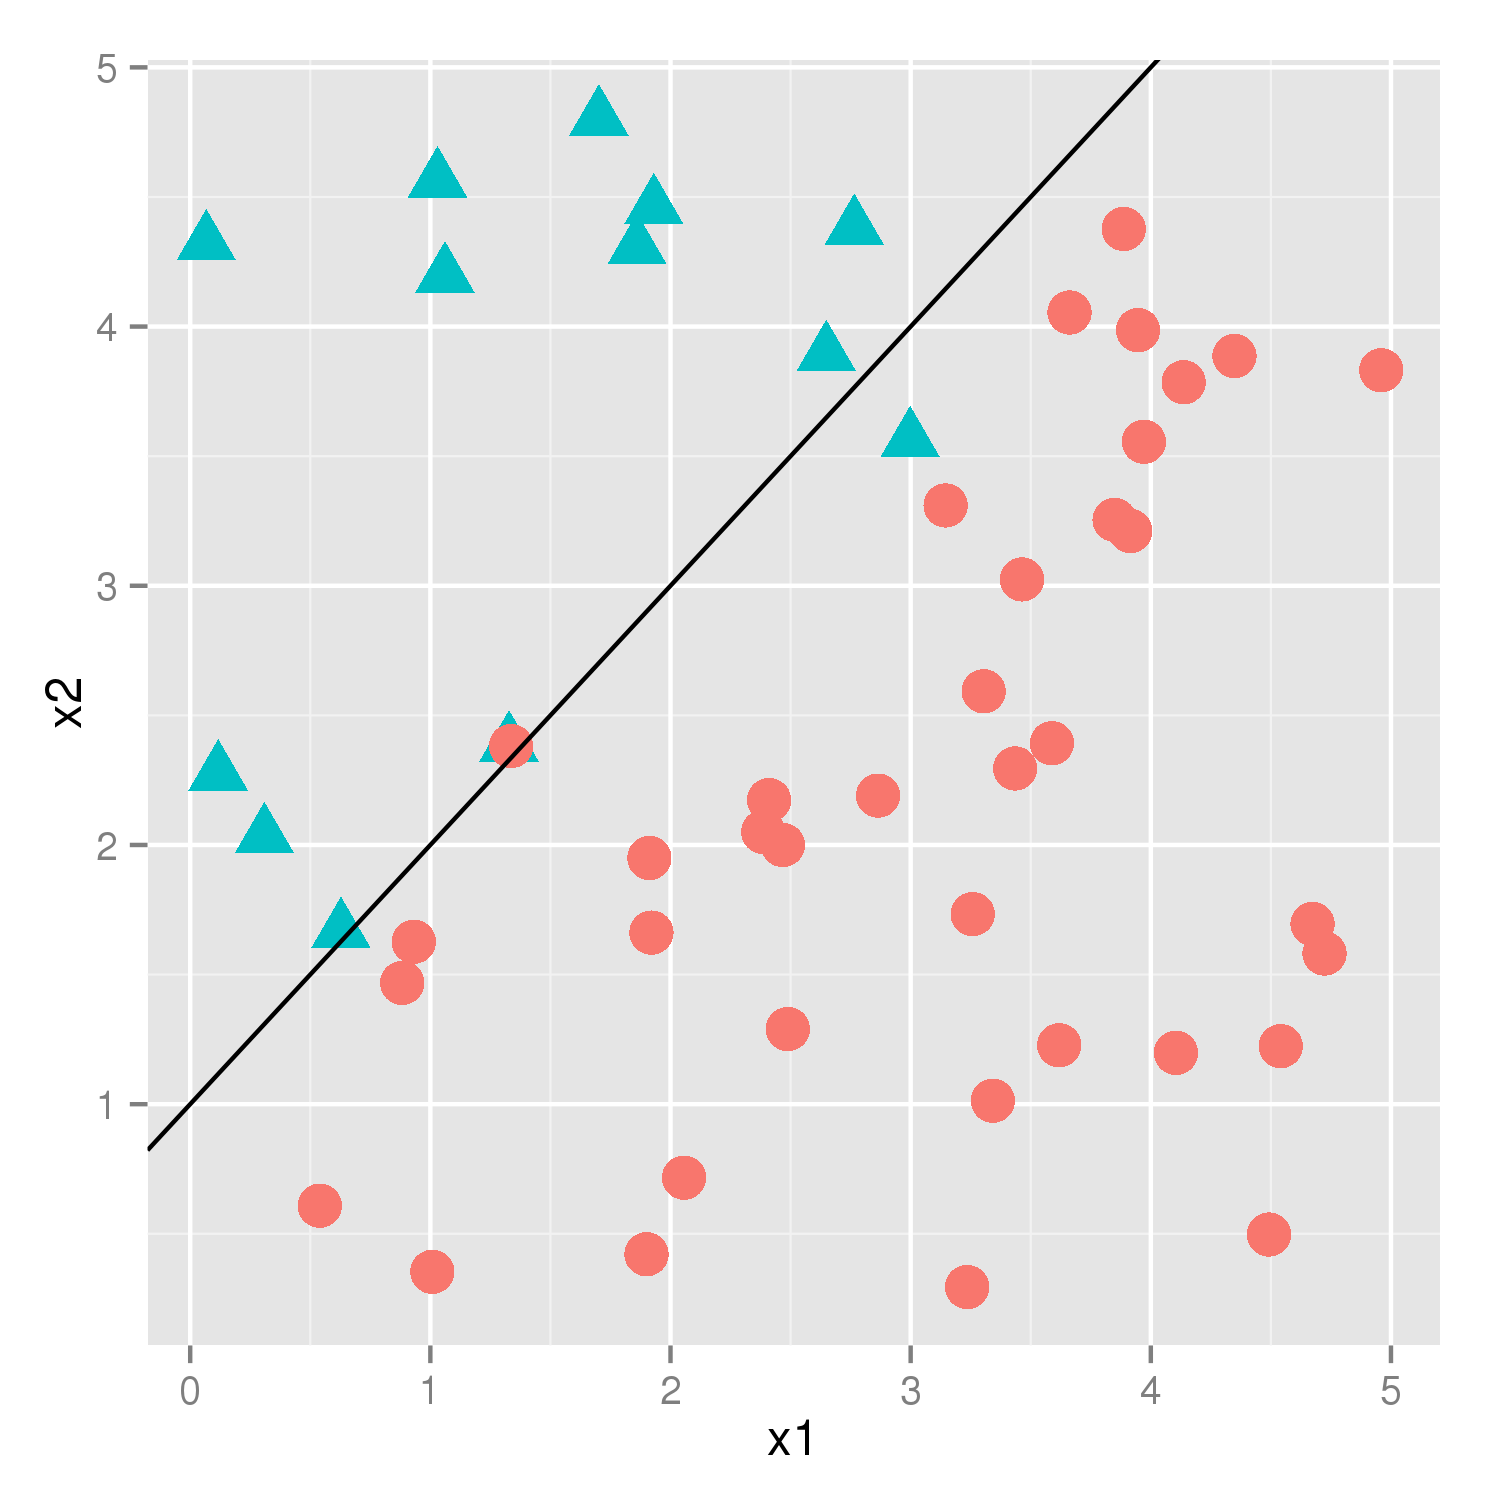
\includegraphics[height=5cm,width=5cm]{decisionboundaries2.png}}
          \end{minipage}
%          &
       \begin{minipage}[t][5cm][t]{4.5cm}
         \footnotesize
     Dos características, $x1$ y $x2$\\
     azul $\leftrightarrow y=1$; rojo $\leftrightarrow y=0$\\
     Tenemos: 
     \begin{itemize}
     \item $\theta=(\theta_0,\theta_1,\theta_2)$,
     \item $x=(1,x_1,x_2)$,
     \end{itemize}
     por lo que la frontera de la región es $$\theta_0+\theta_1x_1+\theta_2x_2=0.$$ Es una recta.
     \end{minipage}\\
%\end{tabular}

 \end{frame}
 \begin{frame}\frametitle{Región de decisión ilustrada con dos características}
 \begin{minipage}[t][5cm][t]{5.5cm}
  \raisebox{-\height}{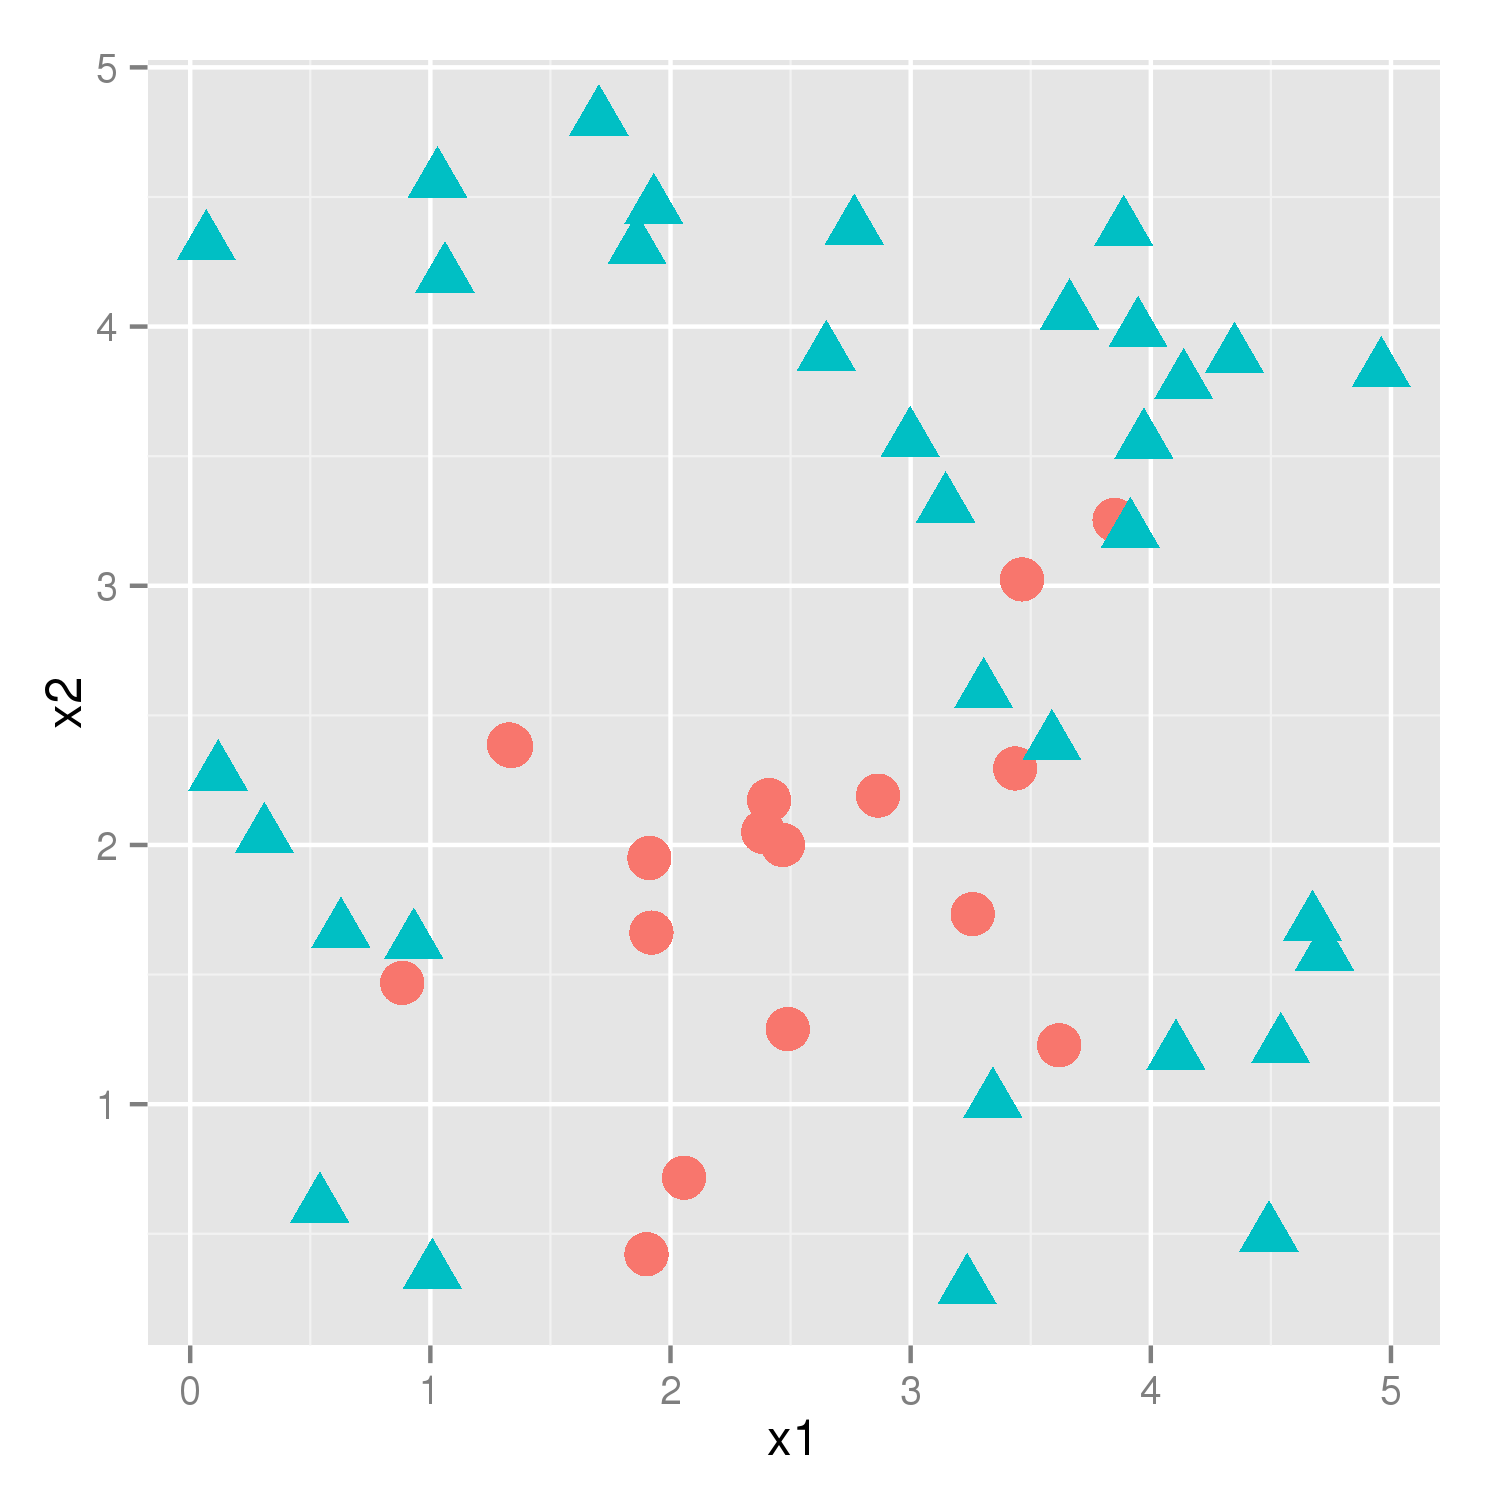
\includegraphics[height=5cm,width=5cm]{decisionboundaries3.png}}
          \end{minipage}
%          &
       \begin{minipage}[t][5cm][t]{4.5cm}
         \footnotesize
     Si introducimos potencias de grado superior de  $x_1$ y $x_2$, podemos obtener fronteras no lineales...
     \begin{itemize}
     \item $\theta=(\theta_0,\theta_1,\theta_2,\theta_3,\theta_4,\theta_5)$,
     \item $x=(1,x_1,x_2,x_1^2,x_1x_2, x_2^2)$,
     \end{itemize}
     
     \end{minipage}\\
%\end{tabular}

 \end{frame}
\begin{frame}\frametitle{Región de decisión ilustrada con dos características}
 \begin{minipage}[t][5cm][t]{5.5cm}
  \raisebox{-\height}{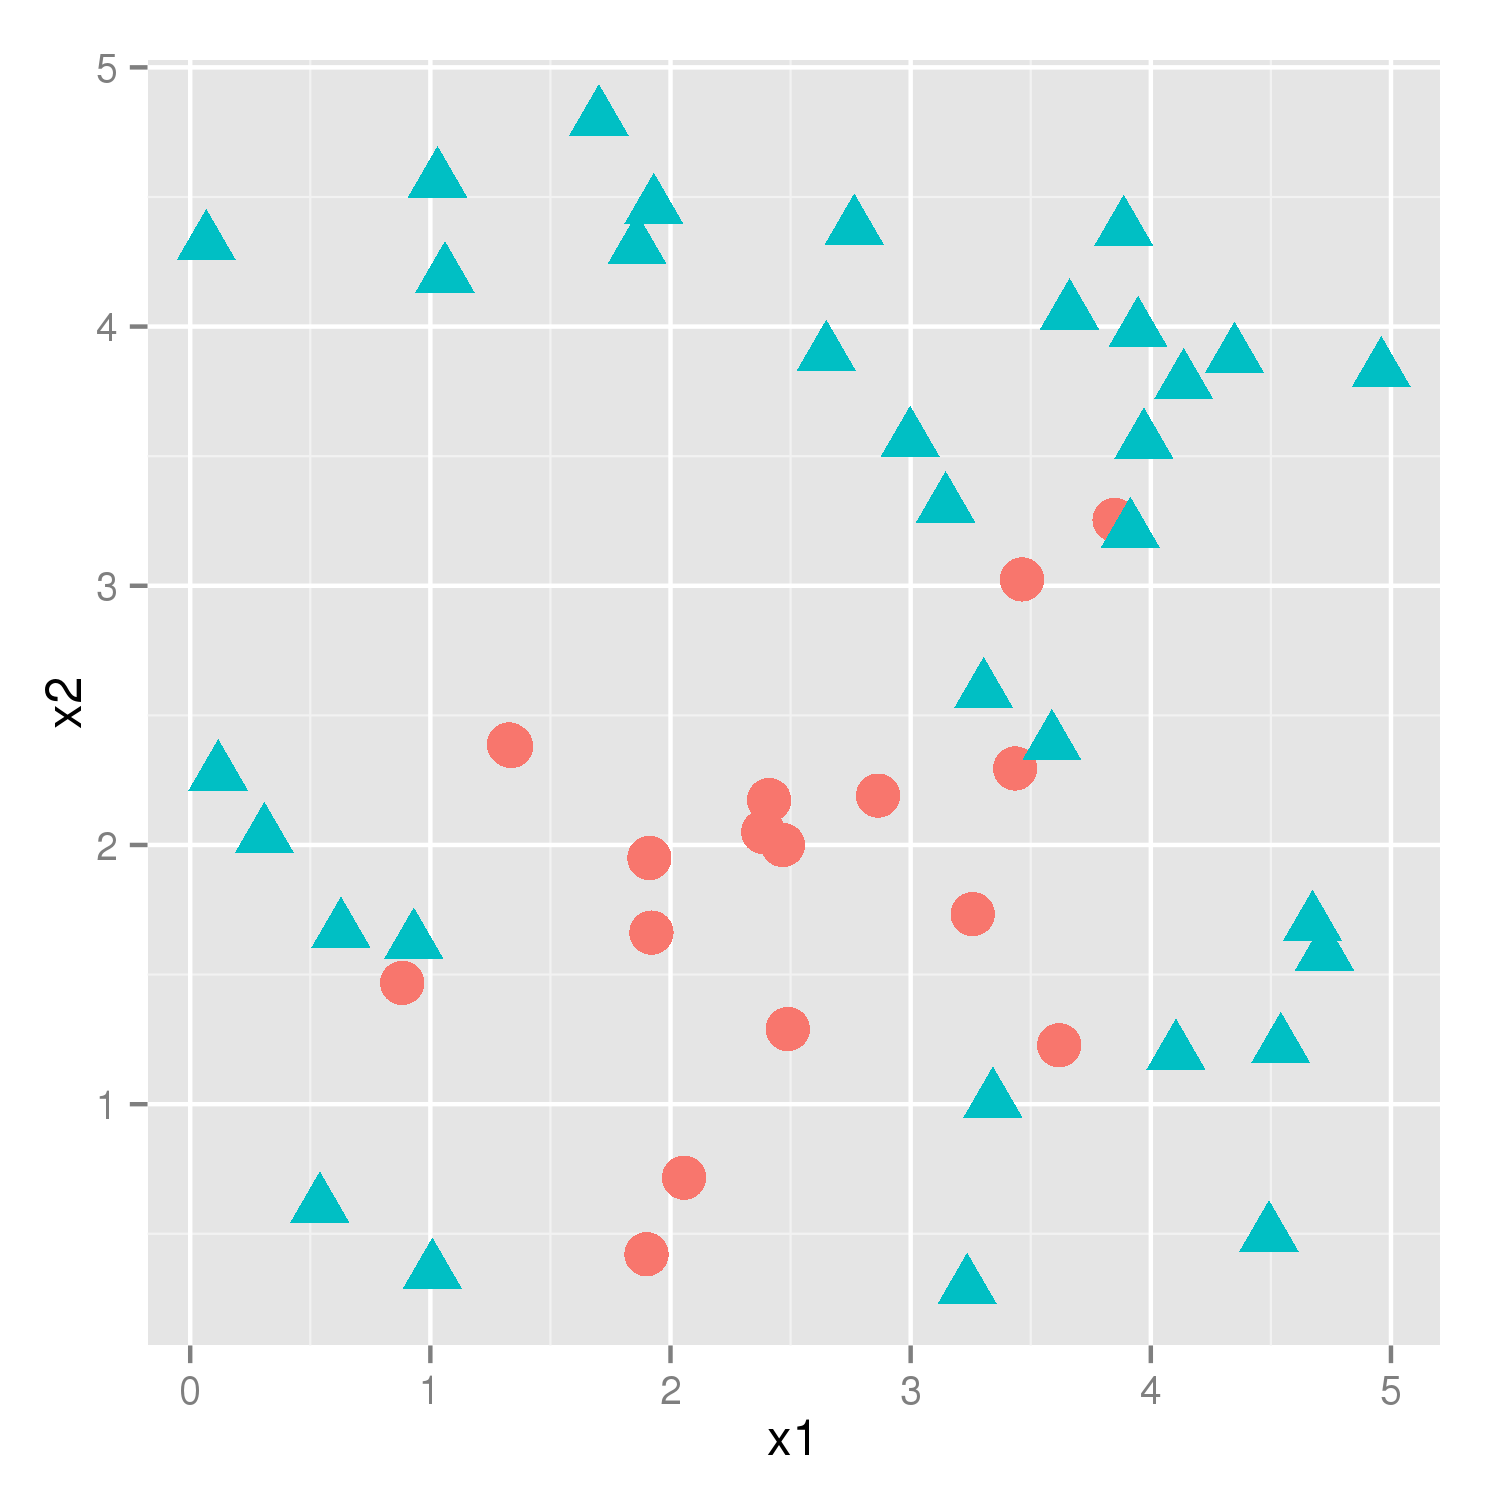
\includegraphics[height=5cm,width=5cm]{decisionboundaries3.png}}
          \end{minipage}
%          &
       \begin{minipage}[t][5cm][t]{4.5cm}
         \footnotesize
     Si introducimos potencias de grado superior de  $x_1$ y $x_2$, podemos obtener fronteras no lineales...
     \begin{itemize}
     \item $\theta=(\theta_0,\theta_1,\theta_2,\theta_3,\theta_4,\theta_5)$,
     \item $x=(1,x_1,x_2,x_1^2,x_1x_2, x_2^2)$,
     \end{itemize}
por lo que la frontera de la región es $$\theta_0+\theta_1x_1+\theta_2x_2+\theta_3x_1^2+\ldots=0.$$

     \end{minipage}\\
%\end{tabular}

 \end{frame}
\begin{frame}\frametitle{Región de decisión ilustrada con dos características}
 \begin{minipage}[t][5cm][t]{5.5cm}
  \raisebox{-\height}{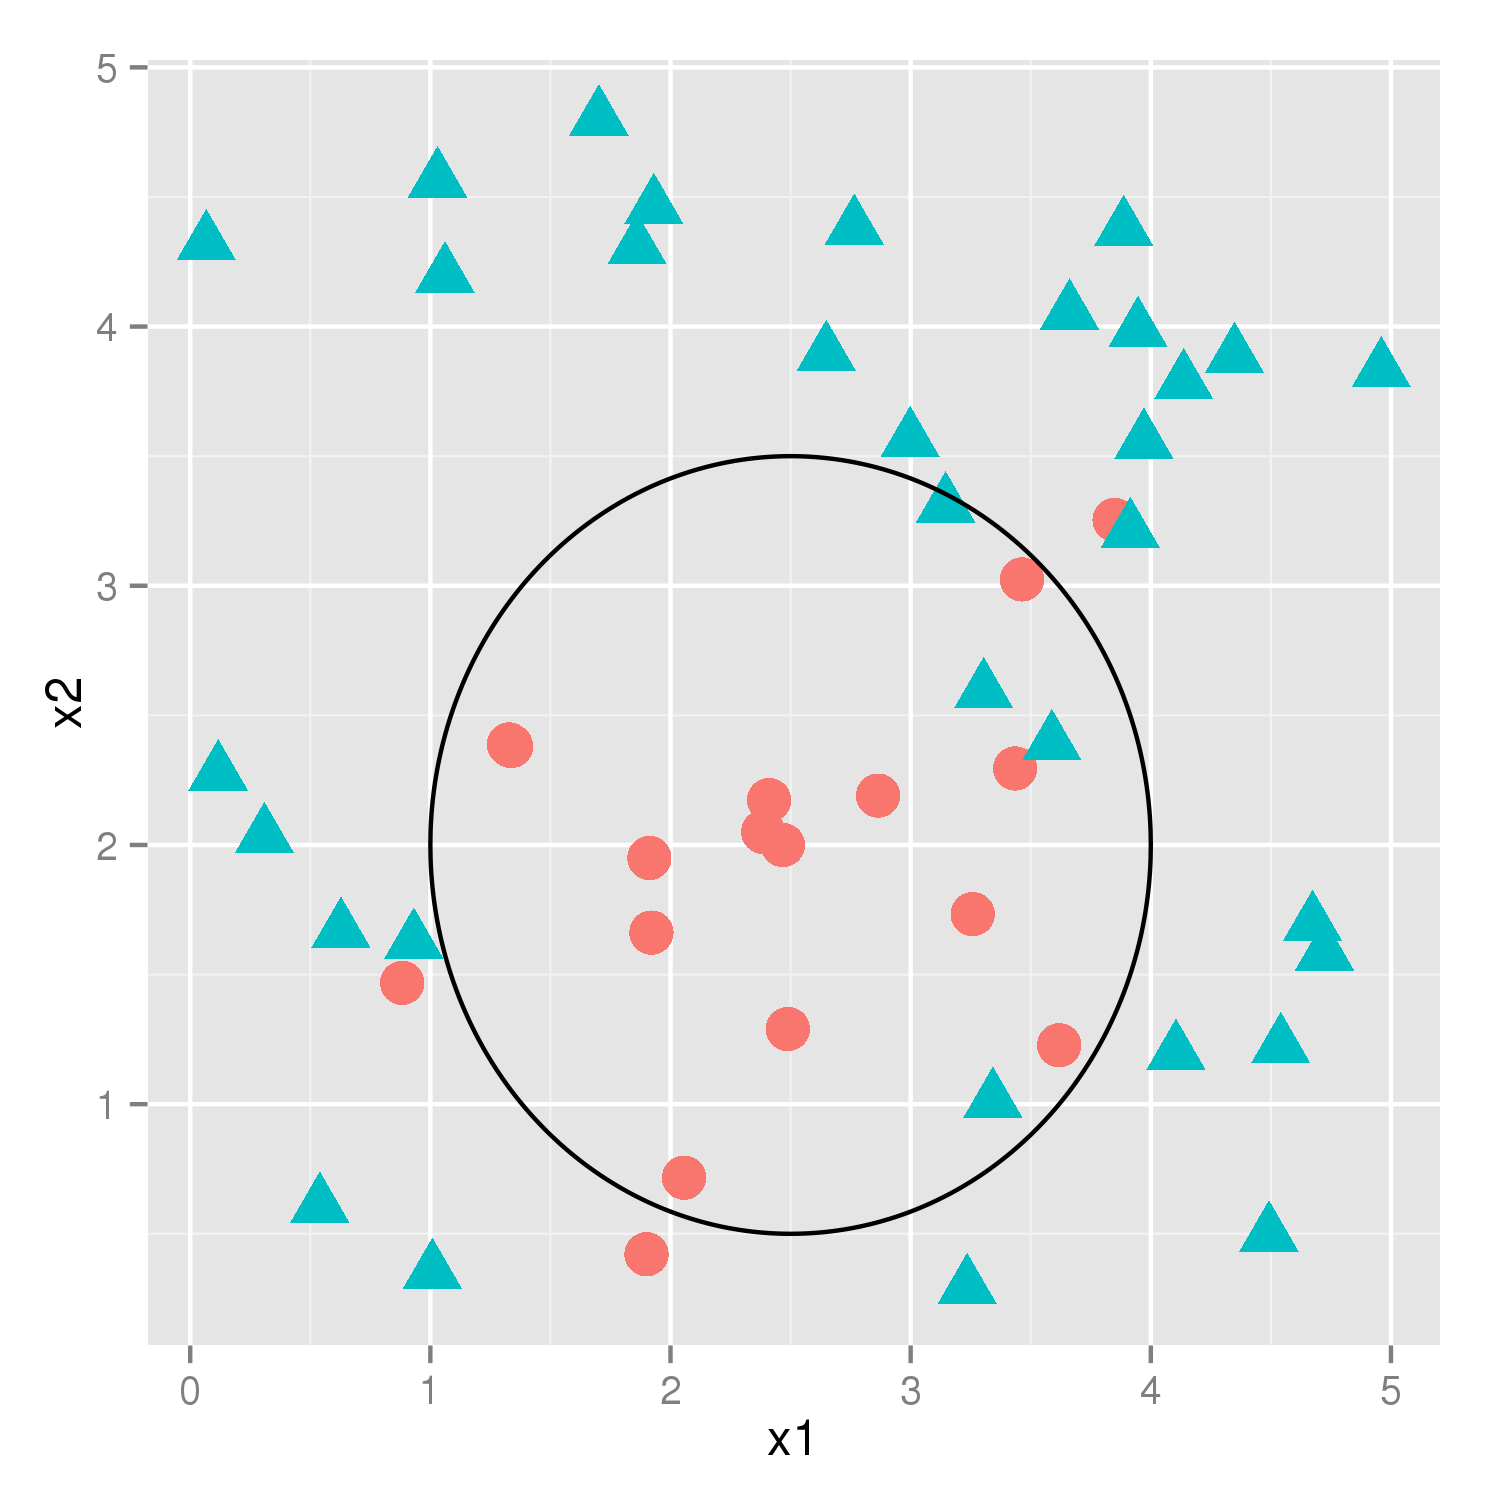
\includegraphics[height=5cm,width=5cm]{decisionboundaries4.png}}
          \end{minipage}
%          &
       \begin{minipage}[t][5cm][t]{4.5cm}
         \footnotesize
     Si introducimos potencias de grado superior de  $x_1$ y $x_2$, podemos obtener fronteras no lineales...
     \begin{itemize}
     \item $\theta=(\theta_0,\theta_1,\theta_2,\theta_3,\theta_4,\theta_5)$,
     \item $x=(1,x_1,x_2,x_1^2,x_1x_2, x_2^2)$,
     \end{itemize}
por lo que la frontera de la región es $$\theta_0+\theta_1x_1+\theta_2x_2+\theta_3x_1^2+\ldots=0.$$
Por ejemplo un círculo...
     \end{minipage}\\
%\end{tabular}
\end{frame}
\begin{frame}\frametitle{Región de decisión ilustrada con dos características}
 \begin{minipage}[t][5cm][t]{5.5cm}
  \raisebox{-\height}{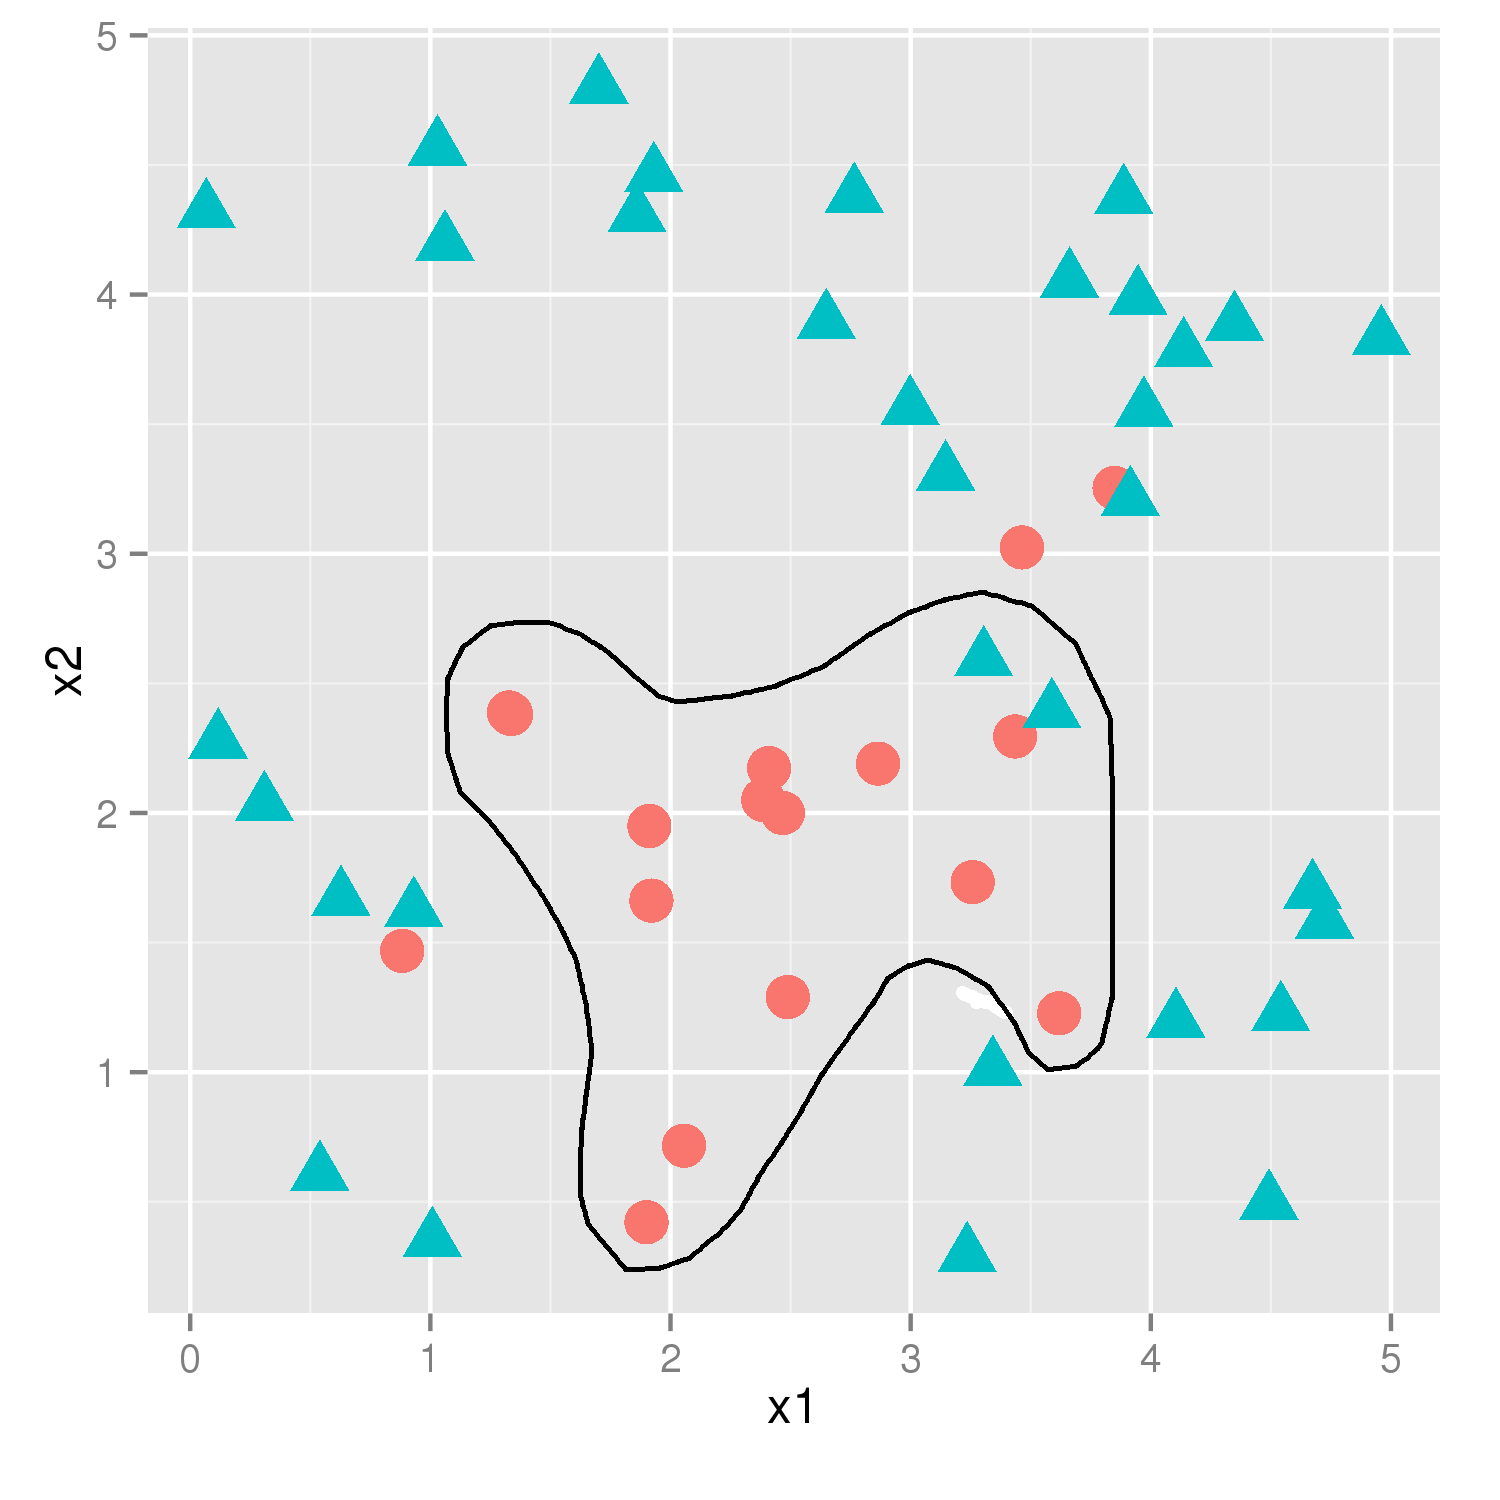
\includegraphics[height=5cm,width=5cm]{decisionboundaries5.png}}
          \end{minipage}
%          &
       \begin{minipage}[t][5cm][t]{4.5cm}
         \footnotesize
     Y si introducimos potencias de grado aun superior $x_1^3$ y $x_2^3\ldots$, $x_1^5$ etc.. podemos obtener fronteras más complejas...
     \end{minipage}\\       
 \end{frame}

\begin{frame}
Conjunto de entrenamiento: los datos que tendremos se presentarán en la forma siguiente:
\begin{center}
  \begin{tabular}{lllll}
  $Y$&$X_1$&$X_2$&$\cdots$&$X_k$\\ \hline
$y_1$&$x_{11}$&$x_{12}$&$\cdots$&$x_{1k}$\\
\vdots&\vdots&\vdots&\vdots&\vdots\\
  $y_{n}$&$x_{n1}$&$x_{n2}$&$\cdots$&$x_{nk}$\\
  \end{tabular}
\end{center}
Cada fila representa un individuo, cada columna una variable o característica para ese individuo.\\
Los valores $y_1$, $y_2$, etc... son valores binarios (0 ó 1).\\
\onslide<2-> Usaremos la notación $$x_{i\bullet}=(x_{i0},x_{i1},\dots,x_{ik})^T$$ para denotar el vector de características del individuo número $i$ \textit{(hemos incluido $x_{i0}=1$.)}

\end{frame}
\section{Coste}
\begin{frame}\frametitle{La función de coste}
  \begin{itemize}
  \item Buscamos entrenar un algoritmo de regresión logística, es decir encontrar el ``mejor'' vector de parámetros $\theta$, aprendiendo de nuestro conjunto de entrenamiento.
  \item<2->   Necesitamos una  función de coste que mida la calidad del ajuste al conjunto de entrenamiento, pero que posea también buenas propiedades para la minimización (convexidad).
  \item<3-> Por ello, introducimos la función de coste siguiente 
$$J(\theta)=\frac 1 n\sum_{i=1}^n coste(h_\theta(x_{i\bullet}),y_i)$$
\onslide<4->
donde 
$$
coste(h_\theta(x),y)= \left\{
\begin{array}{l}
  -\log(h_\theta(x))\quad \mbox{si $y=1$,}\\
  -\log(1-h_\theta(x))\quad \mbox{si $y=0$,}\\
\end{array}\right.
$$
  \end{itemize}
\end{frame}
\begin{frame}\frametitle{La función de coste}
 \begin{minipage}[t][5cm][t]{5.5cm}
  \raisebox{-\height}{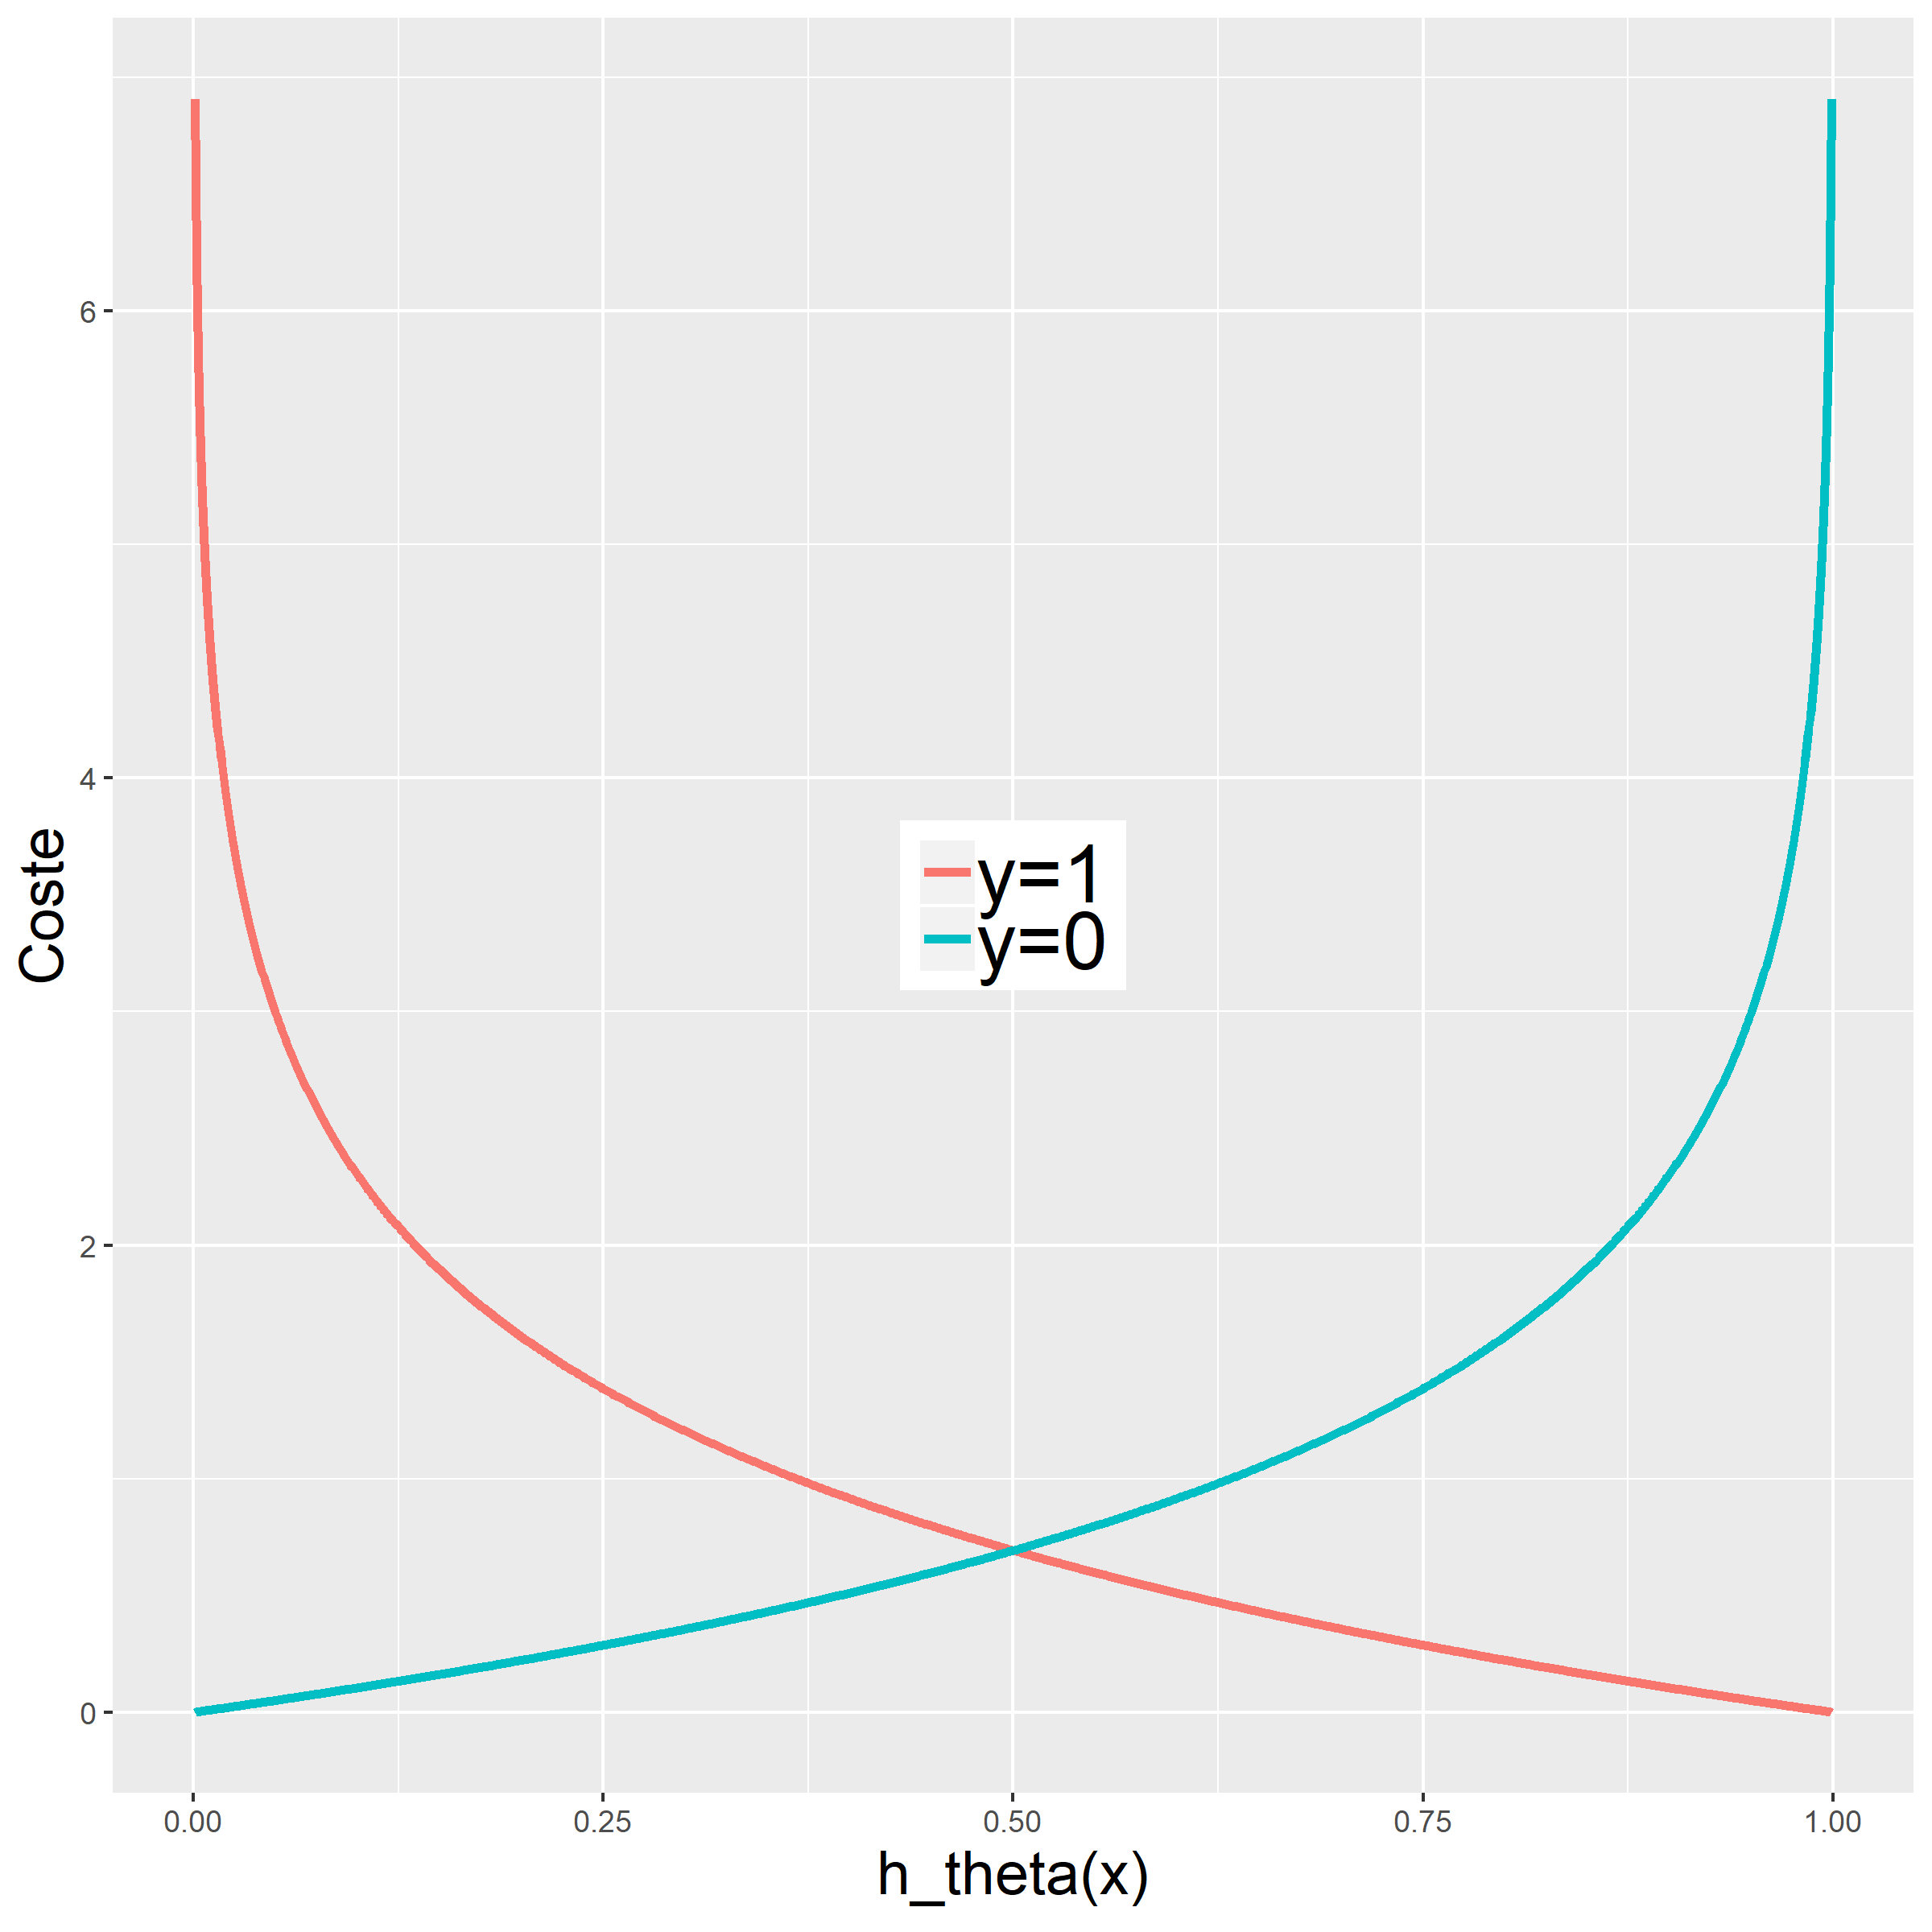
\includegraphics[height=5cm,width=5cm]{costelogistica.png}}
          \end{minipage}
%          &
       \begin{minipage}[t][5cm][t]{5cm}
         \footnotesize
 Este es el perfil de la función de coste.\\
 Por lo tanto: 
 \begin{itemize}
 \item Si $y=1$, cuando $h_\theta(x)\to 0$, $coste(h_\theta(x),y)\to\infty$.
 \item Si $y=1$, cuando $h_\theta(x)=1$, $coste(h_\theta(x),y)=0$.
 \item Si $y=0$, cuando $h_\theta(x)\to 1$, $coste(h_\theta(x),y)\to\infty$.
 \item Si $y=0$, cuando $h_\theta(x)=0$, $coste(h_\theta(x),y)=0$.
 \end{itemize}
     \end{minipage}       
  
\end{frame}
\begin{frame}\frametitle{La función de coste}
  Nuestra función de coste será por lo tanto:
  $$J(\theta)=\frac 1 n\sum_{i=1}^n coste(h_\theta(x_{i\bullet}),y_i)$$
donde 
$$
coste(h_\theta(x),y)= \left\{
\begin{array}{l}
  -\log(h_\theta(x))\quad \mbox{si $y=1$,}\\
  -\log(1-h_\theta(x))\quad \mbox{si $y=0$,}\\
\end{array}\right.,
$$ 
lo que podemos escribir de manera más rápida como
$$J(\theta)=- \frac 1 n\sum_{i=1}^n \left\{y_i\log(h_\theta(x_{i\bullet}))+(1-y_i)\log(1-h_\theta(x_{i\bullet}))\right\}$$
  
\end{frame}
\section{Ajuste}
\begin{frame}\frametitle{Calculo  del gradiente}
Deducimos 
  \begin{eqnarray*}
    \nabla_\theta J(\theta)&=&- \frac 1 n\sum_{i=1}^n \left\{y_i\nabla_\theta\log(h_\theta(x_{i\bullet}))+(1-y_i)\nabla_\theta\log(1-h_\theta(x_{i\bullet}))\right\}\\
    &=& \frac 1 n\sum_{i=1}^n \left\{x_{i\bullet}\cdot (h_\theta(x_{i\bullet})-y_i)\right\}.
  \end{eqnarray*}\onslide<2->
Si usamos la matriz de diseño $\mathbf{X}$, 
  obtenemos  en forma compacta:
   \begin{center}
\fcolorbox{red}{white}{$\displaystyle     \nabla_\theta J(\theta) = \frac 1  n \mathbf{X}^T\cdot\left(\mathbf{H}_\theta-y\right),$}
    \end{center}
\onslide<2-> \scriptsize donde $\mathbf{H}$ denota el vector columna:
$$\mathbf{H}_\theta=\left(
\begin{array}{l}
  h_\theta(x_{1\bullet})\\
  h_\theta(x_{2\bullet})\\
  \vdots\\
  h_\theta(x_{n\bullet})\\
\end{array}\right)$$
\end{frame}

\begin{frame}\frametitle{Nota: comparación con la implementación para regresión múltiple}
Recordad que, para la regresión múltiple, el gradiente era:

   \begin{center}
\fcolorbox{red}{white}{$\displaystyle \nabla_\theta J(\theta) =  \frac
  1  n \mathbf{X}^T\cdot\left(\mathbf{X}\theta-y\right) .$}
    \end{center}
mientras que para la regresión logística, acabamos de establecer que
el gradiente  es:
   \begin{center}
\fcolorbox{red}{white}{$\displaystyle \nabla_\theta J(\theta) = \frac 1  n \mathbf{X}^T\cdot\left(\mathbf{H}_\theta-y\right),$}
    \end{center}
Es muy similar, si queremos programar el algoritmo del gradiente, sólo requiere una pequeña modificación de nuestro código...
\end{frame}
\begin{frame}\frametitle{Regresión logística en {\tt scikit-learn}}
  \begin{block}{}
     Podemos aprovechar la clase {\tt LogisticRegression} del
     submódulo {\tt linear\_model} si no queremos usar algoritmo del gradiente.
  \end{block}
  \onslide<2->
  \begin{itemize}
  \item  Las ventajas:
 \begin{itemize}
 \item No es necesario especificar $\alpha$
 \item Puede ser más rápido.
 \end{itemize}
\item<3-> Sin embargo, en el caso en que haya muchas características,
  puede ser más eficiente usar algoritmo del gradiente ({\tt
    scikit-learn} también dispone de procedimientos para ello.)
  \end{itemize}
\end{frame}
\begin{frame}\frametitle{Si queremos clasificar en más de dos categorías...}
  Si queremos clasificar cada individuo en más de dos categorias, usaremos la técnica del ``One versus all''.\\ \onslide<2->
  {\footnotesize
  \begin{block}{Ejemplo con tres categorías A, B y C.}
    Supongamos que queremos clasificar cada individuo en A, B o C.
    \begin{itemize}
    \item<3-> Entrenamos una regresión logística para clasificar en ``A'' o ``no A''. $\Rightarrow$ obtenemos modelo ajustado $h_{\hat{\theta}_{A}}(x)$.
    \item<4-> Entrenamos una regresión logística para clasificar en ``B'' o ``no B''. $\Rightarrow$ obtenemos modelo ajustado $h_{\hat{\theta}_{B}}(x)$.
    \item<5-> Entrenamos una regresión logística para clasificar en ``C'' o ``no C''. $\Rightarrow$ obtenemos modelo ajustado $h_{\hat{\theta}_{C}}(x)$.
    \item<6-> Dado un nuevo individuo, calculamos las tres probabilidades predichas $h_{\hat{\theta}_{A}}(x)$, $h_{\hat{\theta}_{B}}(x)$ y $h_{\hat{\theta}_{C}}(x)$.
    \item<7-> Clasificamos el individuo en la categoría que tiene la probabilidad predicha más alta...
    \end{itemize}
  \end{block}
  }
\end{frame}
\begin{frame}
  \frametitle{Medir la calidad de la predicción para una clasificación
    binaria}
  El primer indicador que podemos usar es la \alert{tasa de acierto}, es
    decir el porcentaje de individuos clasificados correctamente.
 
  \onslide<2->\footnotesize
  \begin{block}{Ejemplo}
  Consideremos el problema de predecir si un tumor es benigno o
  maligno basándonos en unas imágenes medicales. \\ \onslide<3->
  De un total de 100 tumores, de los cuáles 5 son malignos y 95
  benignos, mi algoritmo se ha equivocado en 1 maligno y 5 benignos.
  \onslide<4->
  $$\mbox{Tasa de acierto} = \frac {94} {100} = 94\%.$$
\end{block}\onslide<5->
Sin embargo, tiene sus limitaciones: si mi decisión hubiera sido
sencillamente declarar todos como benignos, cuál habría sido mi tasa
de acierto? \onslide<6->
  $$\mbox{Tasa de acierto} = \frac {95} {100} = 95\%.$$


\end{frame}

\begin{frame}
  \frametitle{Precisión y sensibilidad (``recall'')}
  Por ello, introducimos dos indicadores que debemos considerar conjuntamente:
 
  \onslide<2->\footnotesize
  \begin{block}{Precisión}
  Es la proporción  de  aciertos ($y=1$) entre los que he clasificado como
  ``positivos'' ($\hat y=1$). 
\end{block}\onslide<3->
  \begin{block}{Sensibilidad ``Recall''}
  Es la proporción de aciertos ($\hat y=1$) entre todos los que son positivos
  ``positivos'' ($y=1$). 
\end{block}\onslide<4->
Para el problema anterior: De un total de 100 tumores, de los cuáles 5 son malignos y 95
  benignos, mi algoritmo se ha equivocado en 1 maligno y 5 benignos.\onslide<5->
  $$precision = 4 / 9, \qquad recall = 4 / 5$$\onslide<6->
  Si los declaro todos como benignos:
  $$precision = \mbox{no existe}, \qquad recall = 0 / 5= 0$$\onslide<6->
  
\end{frame}

\begin{frame}
  \frametitle{Matriz de confusión}
  Se suele presentar los resultados del algoritmo en forma de matriz,
  llamada matriz de confusión.\\ \onslide<2->
  Para el problema anterior: De un total de 100 tumores, de los cuáles 5 son malignos y 95
  benignos, mi algoritmo se ha equivocado en 1 maligno y 5 benignos.\onslide<3->
\begin{center}
  \begin{tabular}[h]{l||ll}
      $y \backslash \hat y$&0&1\\ \hline\hline
      0&90&5\\
      1&1&4\\
    \end{tabular}
  \end{center}
  \onslide<4->
  Matriz de confusión:
   $$\left(
     \begin{array}[h]{ll}
       90&5\\
       1&4\\
     \end{array}
   \right)$$
 \end{frame}
 \begin{frame}
   \frametitle{Precisión y sensibilidad}
   La precisión y la sensibilidad van en sentido contrario: si aumenta
   la precisión, baja la sensibilidad y al revés.\onslide<2->\\
   Se busca un equilibrio.
   \onslide<3->
   Dos características y una frontera de decisión lineal:\\
   \begin{center}
     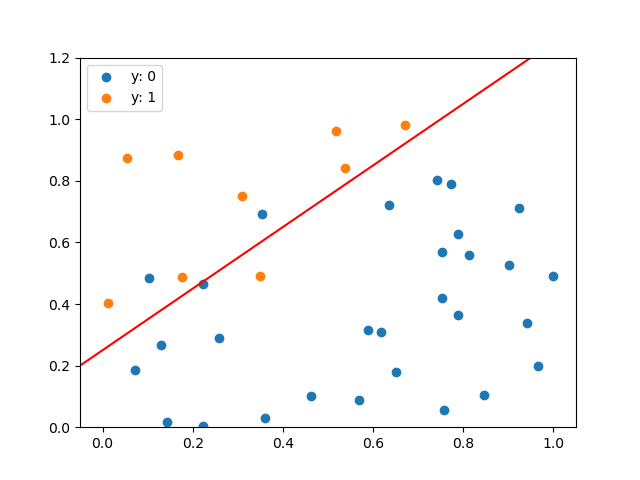
\includegraphics[height=5cm,width=5cm]{precision_recall.png}
   \end{center}\onslide<4->
         Tenemos una precisión de 80\% y una sensibilidad de 8/9, (89\%).

   
 \end{frame}
\begin{frame}
   \frametitle{Precisión y sensibilidad}
   La precisión y la sensibilidad van en sentido contrario: si aumenta
   la precisión, baja la sensibilidad y al revés.\\
   Se busca un equilibrio.
   Dos características y una frontera de decisión lineal. {\footnotesize
     Si aumento
   la ordenada al origen de la frontera:}\\
   \begin{center}
     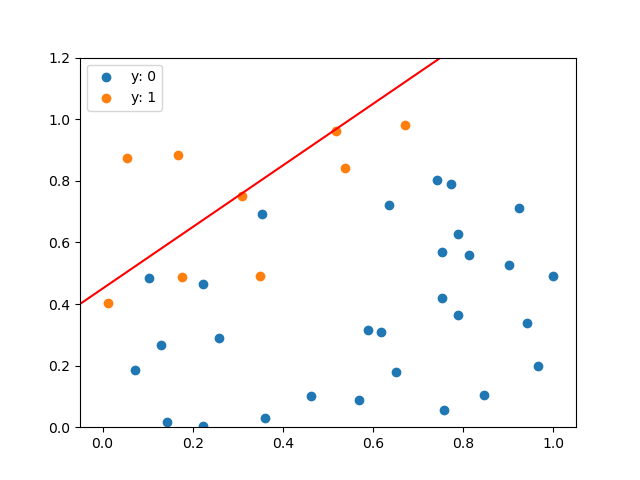
\includegraphics[height=5cm,width=5cm]{precision_recall_1.png}
   \end{center}\onslide<2->
         Tenemos una precisión de 100\% y una sensibilidad de 2/9 (22\%)

   
 \end{frame}

\begin{frame}
   \frametitle{Precisión y sensibilidad}
   La precisión y la sensibilidad van en sentido contrario: si aumenta
   la precisión, baja la sensibilidad y al revés.\\
   Se busca un equilibrio.
   Dos características y una frontera de decisión lineal. {\footnotesize
     Si disminuyo
   la ordenada al origen de la frontera:}\\
   \begin{center}
     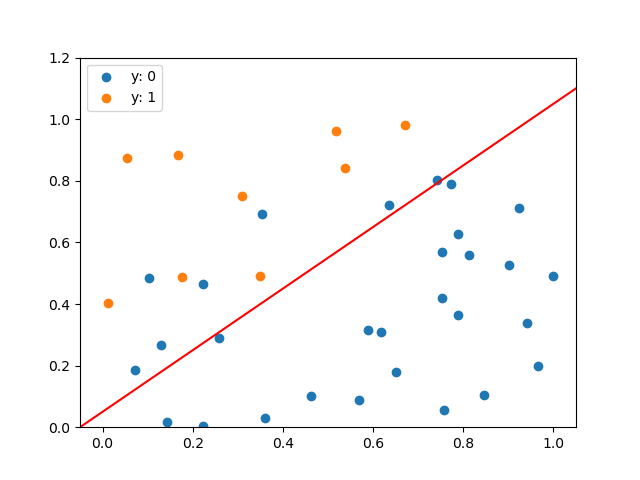
\includegraphics[height=5cm,width=5cm]{precision_recall_2.png}
   \end{center}\onslide<2->
         Tenemos una precisión de 64\% y una sensibilidad de 100\%

   
 \end{frame}
\begin{frame}
   \frametitle{Precisión y sensibilidad}
   Una tipica situación: \onslide<2->
   \begin{center}
     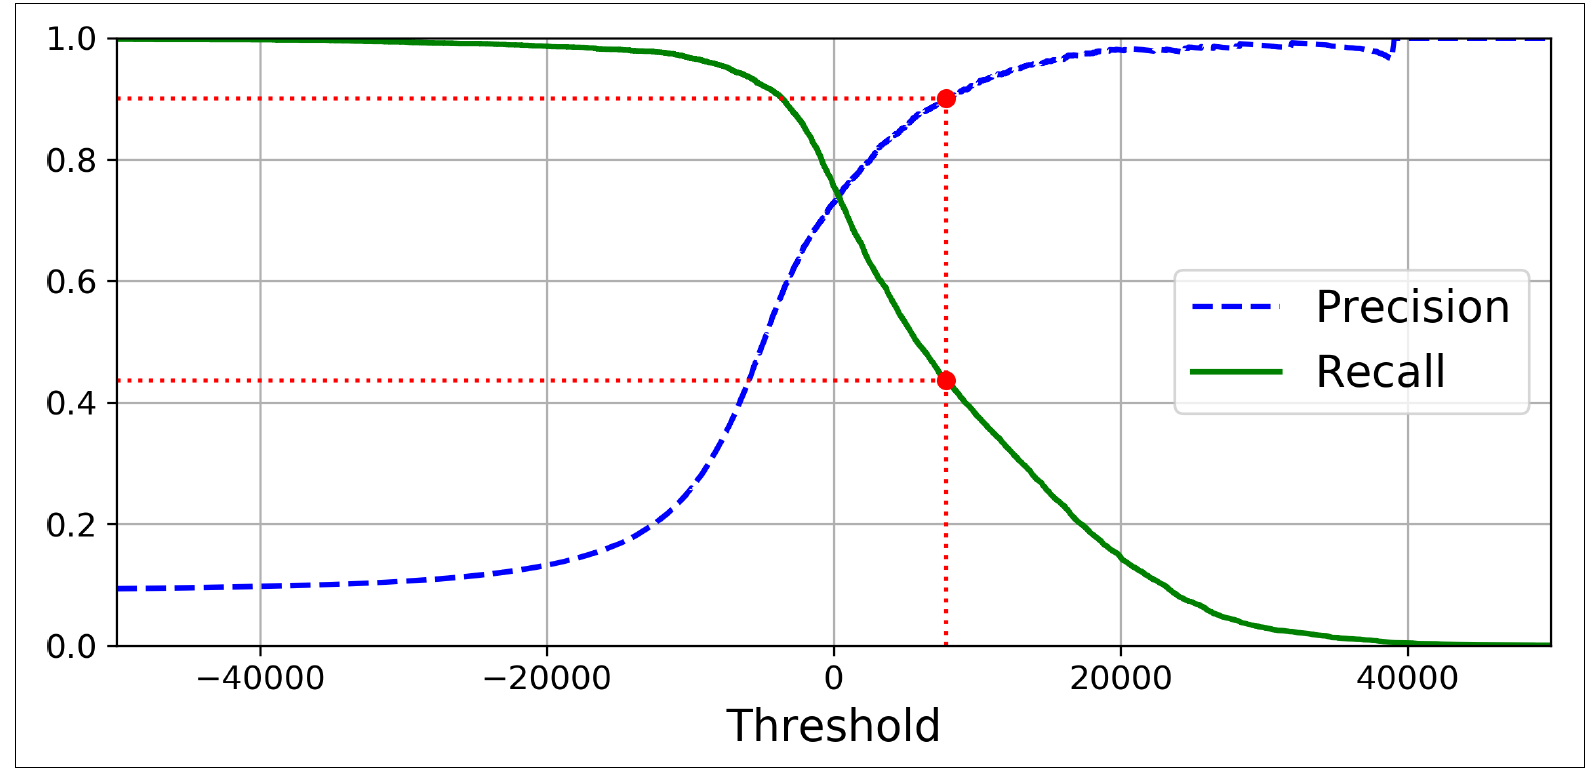
\includegraphics[width=8cm]{precision-recall-curve.png}
   \end{center}
   {\tiny Fuente: https://jaehyeongan.github.io/2020/02/29/LSTM-Autoencoder-for-Anomaly-Detection/}

   
 \end{frame}
\end{document}
